\documentclass[twoside]{book}

% Packages required by doxygen
\usepackage{fixltx2e}
\usepackage{calc}
\usepackage{doxygen}
\usepackage[export]{adjustbox} % also loads graphicx
\usepackage{graphicx}
\usepackage[utf8]{inputenc}
\usepackage{makeidx}
\usepackage{multicol}
\usepackage{multirow}
\PassOptionsToPackage{warn}{textcomp}
\usepackage{textcomp}
\usepackage[nointegrals]{wasysym}
\usepackage[table]{xcolor}

% Font selection
\usepackage[T1]{fontenc}
\usepackage[scaled=.90]{helvet}
\usepackage{courier}
\usepackage{amssymb}
\usepackage{sectsty}
\renewcommand{\familydefault}{\sfdefault}
\allsectionsfont{%
  \fontseries{bc}\selectfont%
  \color{darkgray}%
}
\renewcommand{\DoxyLabelFont}{%
  \fontseries{bc}\selectfont%
  \color{darkgray}%
}
\newcommand{\+}{\discretionary{\mbox{\scriptsize$\hookleftarrow$}}{}{}}

% Page & text layout
\usepackage{geometry}
\geometry{%
  a4paper,%
  top=2.5cm,%
  bottom=2.5cm,%
  left=2.5cm,%
  right=2.5cm%
}
\tolerance=750
\hfuzz=15pt
\hbadness=750
\setlength{\emergencystretch}{15pt}
\setlength{\parindent}{0cm}
\setlength{\parskip}{3ex plus 2ex minus 2ex}
\makeatletter
\renewcommand{\paragraph}{%
  \@startsection{paragraph}{4}{0ex}{-1.0ex}{1.0ex}{%
    \normalfont\normalsize\bfseries\SS@parafont%
  }%
}
\renewcommand{\subparagraph}{%
  \@startsection{subparagraph}{5}{0ex}{-1.0ex}{1.0ex}{%
    \normalfont\normalsize\bfseries\SS@subparafont%
  }%
}
\makeatother

% Headers & footers
\usepackage{fancyhdr}
\pagestyle{fancyplain}
\fancyhead[LE]{\fancyplain{}{\bfseries\thepage}}
\fancyhead[CE]{\fancyplain{}{}}
\fancyhead[RE]{\fancyplain{}{\bfseries\leftmark}}
\fancyhead[LO]{\fancyplain{}{\bfseries\rightmark}}
\fancyhead[CO]{\fancyplain{}{}}
\fancyhead[RO]{\fancyplain{}{\bfseries\thepage}}
\fancyfoot[LE]{\fancyplain{}{}}
\fancyfoot[CE]{\fancyplain{}{}}
\fancyfoot[RE]{\fancyplain{}{\bfseries\scriptsize Generated by Doxygen }}
\fancyfoot[LO]{\fancyplain{}{\bfseries\scriptsize Generated by Doxygen }}
\fancyfoot[CO]{\fancyplain{}{}}
\fancyfoot[RO]{\fancyplain{}{}}
\renewcommand{\footrulewidth}{0.4pt}
\renewcommand{\chaptermark}[1]{%
  \markboth{#1}{}%
}
\renewcommand{\sectionmark}[1]{%
  \markright{\thesection\ #1}%
}

% Indices & bibliography
\usepackage{natbib}
\usepackage[titles]{tocloft}
\setcounter{tocdepth}{3}
\setcounter{secnumdepth}{5}
\makeindex

% Hyperlinks (required, but should be loaded last)
\usepackage{ifpdf}
\ifpdf
  \usepackage[pdftex,pagebackref=true]{hyperref}
\else
  \usepackage[ps2pdf,pagebackref=true]{hyperref}
\fi
\hypersetup{%
  colorlinks=true,%
  linkcolor=blue,%
  citecolor=blue,%
  unicode%
}

% Custom commands
\newcommand{\clearemptydoublepage}{%
  \newpage{\pagestyle{empty}\cleardoublepage}%
}

\usepackage{caption}
\captionsetup{labelsep=space,justification=centering,font={bf},singlelinecheck=off,skip=4pt,position=top}

%===== C O N T E N T S =====

\begin{document}

% Titlepage & ToC
\hypersetup{pageanchor=false,
             bookmarksnumbered=true,
             pdfencoding=unicode
            }
\pagenumbering{alph}
\begin{titlepage}
\vspace*{7cm}
\begin{center}%
{\Large Matrice210\+Pi }\\
\vspace*{1cm}
{\large Generated by Doxygen 1.8.14}\\
\end{center}
\end{titlepage}
\clearemptydoublepage
\pagenumbering{roman}
\tableofcontents
\clearemptydoublepage
\pagenumbering{arabic}
\hypersetup{pageanchor=true}

%--- Begin generated contents ---
\chapter{Matrice210\+Pi}
\label{index}\hypertarget{index}{}This code uses D\+JI Onboard S\+DK to communicate with D\+JI flight controllers.

More information can be found in readme.\+md file\hypertarget{index_Architecture}{}\section{Architecture}\label{index_Architecture}
   
\chapter{Matrice210\+Pi}
\label{md__r_e_a_d_m_e}
\Hypertarget{md__r_e_a_d_m_e}
This code uses \href{https://github.com/dji-sdk/Onboard-SDK/}{\tt D\+JI Onboard S\+DK} to communicate with D\+JI flight controllers.

\subsection*{Prerequisites}

Code compiled with \href{https://cmake.org/}{\tt C\+Make} 3.\+7.\+2 on a \href{https://www.raspberrypi.org/products/raspberry-pi-zero-w/}{\tt Raspberry Pi Zero W} with \href{https://www.raspberrypi.org/downloads/raspbian/}{\tt Raspbian Stretch Lite} (June 2018 -\/ Kernel version\+:4.\+14).

\subsubsection*{U\+A\+RT}

\href{https://github.com/dji-sdk/Onboard-SDK/}{\tt D\+JI Onboard S\+DK} uses serial U\+A\+RT driver to communicate with D\+JI flight controllers. The U\+A\+RT transmit and receive pins are on G\+P\+IO 14 and G\+P\+IO 15 respectively, which are pins 8 and 10 on the G\+P\+IO header.

In a default install of Raspbian on a Raspberry, the primary U\+A\+RT {\ttfamily /dev/serial0} is assigned to the Linux console. To stop this behaviour, the serial console setting needs to be removed from command line. This can be done using the https\+://www.raspberrypi.\+org/documentation/configuration/raspi-\/config.md \char`\"{}raspi-\/config\char`\"{} \+:


\begin{DoxyCode}
sudo raspi-config
\end{DoxyCode}
 Select option 5, {\bfseries Interfacing options}, then option {\bfseries Serial}, then {\bfseries Disable serial login shell} (disable linux\textquotesingle{}s use of console uart) and {\bfseries Enable serial interface}. Exit raspi-\/config and reboot

\subsubsection*{U\+A\+RT by U\+SB}

The \href{https://www.st.com/en/evaluation-tools/32f429idiscovery.html}{\tt 32\+F429\+I\+D\+I\+S\+C\+O\+V\+E\+RY} card used by the embedded sensor transmits values by U\+A\+RT. It is connected to a U\+S\+B-\/\+T\+TL adaptator and uses U\+SB User port {\ttfamily /dev/tty\+U\+S\+B0} on the Pi Zero W.

\subsection*{Install}

Clone the \href{https://github.com/dji-sdk/Onboard-SDK/}{\tt D\+JI Onboard S\+DK} repository and configure {\ttfamily O\+N\+B\+O\+A\+R\+D\+S\+D\+K\+\_\+\+S\+O\+U\+R\+CE} in \href{CMakeLists.txt}{\tt C\+Make\+List.\+txt} depending on your repository location.

In the {\ttfamily Matrice210\+Pi} root directory, run the following commands to build the app\+: 
\begin{DoxyCode}
mkdir build && cd build
cmake ..
make
cd bin
\end{DoxyCode}


You have to copy the {\ttfamily User\+Config.\+txt} file provided by D\+JI in the {\ttfamily bin} directory and fill it in with your configuration informations. You must register as a developer with D\+JI and create an O\+S\+DK application ID and Key pair, see \href{https://developer.dji.com/onboard-sdk/documentation/development-workflow/environment-setup.html#onboard-sdk-application-registration}{\tt here}.

Be sure Onboard S\+DK is enabled on the aircraft and the baudrate used in {\ttfamily User\+Config.\+txt} file is the same as defined with D\+JI Assistant 2, more informations \href{https://developer.dji.com/onboard-sdk/documentation/development-workflow/environment-setup.html}{\tt here}.

More informations can be found in the \href{https://developer.dji.com/onboard-sdk/documentation/quick-start/quick-start.html}{\tt Quick start Guide} or in the \href{https://developer.dji.com/onboard-sdk/documentation/introduction/homepage.html}{\tt D\+JI documentation}.

You can then launch program in {\ttfamily bin} directory with 
\begin{DoxyCode}
sudo ./matrice210 1
\end{DoxyCode}


If the program is launched with {\ttfamily sudo ./matrice210 0}, the console interface is not displayed.

\subsection*{Result}

The following interface is shown in the program console when console is enabled.



Due to the watchdog, if the program is launched after the Android Application on the mobile device, data may be received before full program initialization.



If console is disabled, {\ttfamily Available commands} are not displayed.

\subsection*{Linux service}

The \href{Linux/runMatrice210.sh}{\tt run\+Matrice210.\+sh} script can be automatically launched from a service on Pi start-\/up if the \href{Linux/matrice210.service}{\tt matrice210.\+service} is added in {\ttfamily /etc/systemd/system}. Linux service can then be \href{Linux/stopMatrice210.sh}{\tt stopped} and \href{Linux/startMatrice210.sh}{\tt restarted} with dedicated script files

\subsection*{Log}

The \href{Linux/runMatrice210.sh}{\tt run\+Matrice210.\+sh} saves console output in {\ttfamily build/bin/log/} directory. Logs are formatting as follow \+: {\ttfamily log\mbox{[}index\mbox{]}-\/\mbox{[}yyyy\mbox{]}\mbox{[}mm\mbox{]}\mbox{[}dd\mbox{]}-\/\mbox{[}hh\mbox{]}\mbox{[}mm\mbox{]}\mbox{[}ss\mbox{]}.log}. G\+MT Date/\+Time is used, {\ttfamily index} is incremented to have numbered log and last log starts with \+\_\+ char.

The current log file can be read in real time with command {\ttfamily tail -\/f \+\_\+$\ast$.log}.

\subsection*{Usage}

For full compatibility, use this code with the \href{https://github.com/jonathanmichel/Matrice210Android}{\tt Matrice210\+Android\+App} on an Android device connected to aircraft remote controller and the \href{https://github.com/jonathanmichel/Matrice210Stm32}{\tt Matrice210\+Stm32} code running on a \href{https://www.st.com/en/evaluation-tools/32f429idiscovery.html}{\tt S\+T\+M32\+F429\+I\+D\+I\+S\+C\+O\+V\+E\+RY board}.

\subsection*{Authors}


\begin{DoxyItemize}
\item {\bfseries Jonathan Michel} -\/ {\itshape Initial work} -\/ \href{https://github.com/jonathanmichel}{\tt jonathanmichel} 
\end{DoxyItemize}
\chapter{Hierarchical Index}
\section{Class Hierarchy}
This inheritance list is sorted roughly, but not completely, alphabetically\+:\begin{DoxyCompactList}
\item \contentsline{section}{M210\+:\+:Action\+Data}{\pageref{class_m210_1_1_action_data}}{}
\item \contentsline{section}{M210\+:\+:Avalanche\+Mission}{\pageref{class_m210_1_1_avalanche_mission}}{}
\item \contentsline{section}{M210\+:\+:Console}{\pageref{class_m210_1_1_console}}{}
\item \contentsline{section}{M210\+:\+:Dms}{\pageref{struct_m210_1_1_dms}}{}
\item \contentsline{section}{M210\+:\+:Emergency}{\pageref{class_m210_1_1_emergency}}{}
\item \contentsline{section}{M210\+:\+:Flight\+Controller}{\pageref{class_m210_1_1_flight_controller}}{}
\item \contentsline{section}{M210\+:\+:Geodetic\+Coord}{\pageref{class_m210_1_1_geodetic_coord}}{}
\item \contentsline{section}{M210\+:\+:Gps\+Manip}{\pageref{class_m210_1_1_gps_manip}}{}
\item \contentsline{section}{M210\+:\+:Mobile}{\pageref{class_m210_1_1_mobile}}{}
\item \contentsline{section}{M210\+:\+:Monitored\+Mission}{\pageref{class_m210_1_1_monitored_mission}}{}
\item \contentsline{section}{M210\+:\+:Position\+Mission}{\pageref{class_m210_1_1_position_mission}}{}
\item \contentsline{section}{M210\+:\+:Position\+Offset\+Mission}{\pageref{class_m210_1_1_position_offset_mission}}{}
\item Singleton\begin{DoxyCompactList}
\item \contentsline{section}{M210\+:\+:Action}{\pageref{class_m210_1_1_action}}{}
\item \contentsline{section}{M210\+:\+:Gps\+Axis}{\pageref{class_m210_1_1_gps_axis}}{}
\item \contentsline{section}{M210\+:\+:Log}{\pageref{class_m210_1_1_log}}{}
\item \contentsline{section}{M210\+:\+:Package\+Manager}{\pageref{class_m210_1_1_package_manager}}{}
\end{DoxyCompactList}
\item \contentsline{section}{M210\+:\+:Thread\+Manager}{\pageref{class_m210_1_1_thread_manager}}{}
\item \contentsline{section}{M210\+:\+:Uart}{\pageref{class_m210_1_1_uart}}{}
\item \contentsline{section}{Vector2}{\pageref{struct_vector2}}{}
\item \contentsline{section}{M210\+:\+:Velocity\+Mission}{\pageref{class_m210_1_1_velocity_mission}}{}
\item \contentsline{section}{M210\+:\+:Watchdog}{\pageref{class_m210_1_1_watchdog}}{}
\item \contentsline{section}{M210\+:\+:Waypoint\+Mission}{\pageref{class_m210_1_1_waypoint_mission}}{}
\end{DoxyCompactList}

\chapter{Class Index}
\section{Class List}
Here are the classes, structs, unions and interfaces with brief descriptions\+:\begin{DoxyCompactList}
\item\contentsline{section}{\mbox{\hyperlink{class_m210_1_1_action}{M210\+::\+Action}} }{\pageref{class_m210_1_1_action}}{}
\item\contentsline{section}{\mbox{\hyperlink{class_m210_1_1_action_data}{M210\+::\+Action\+Data}} }{\pageref{class_m210_1_1_action_data}}{}
\item\contentsline{section}{\mbox{\hyperlink{class_m210_1_1_avalanche_mission}{M210\+::\+Avalanche\+Mission}} }{\pageref{class_m210_1_1_avalanche_mission}}{}
\item\contentsline{section}{\mbox{\hyperlink{class_m210_1_1_console}{M210\+::\+Console}} }{\pageref{class_m210_1_1_console}}{}
\item\contentsline{section}{\mbox{\hyperlink{struct_m210_1_1_dms}{M210\+::\+Dms}} }{\pageref{struct_m210_1_1_dms}}{}
\item\contentsline{section}{\mbox{\hyperlink{class_m210_1_1_emergency}{M210\+::\+Emergency}} }{\pageref{class_m210_1_1_emergency}}{}
\item\contentsline{section}{\mbox{\hyperlink{class_m210_1_1_flight_controller}{M210\+::\+Flight\+Controller}} }{\pageref{class_m210_1_1_flight_controller}}{}
\item\contentsline{section}{\mbox{\hyperlink{class_m210_1_1_geodetic_coord}{M210\+::\+Geodetic\+Coord}} }{\pageref{class_m210_1_1_geodetic_coord}}{}
\item\contentsline{section}{\mbox{\hyperlink{class_m210_1_1_gps_axis}{M210\+::\+Gps\+Axis}} }{\pageref{class_m210_1_1_gps_axis}}{}
\item\contentsline{section}{\mbox{\hyperlink{class_m210_1_1_gps_manip}{M210\+::\+Gps\+Manip}} }{\pageref{class_m210_1_1_gps_manip}}{}
\item\contentsline{section}{\mbox{\hyperlink{class_m210_1_1_log}{M210\+::\+Log}} }{\pageref{class_m210_1_1_log}}{}
\item\contentsline{section}{\mbox{\hyperlink{class_m210_1_1_mobile}{M210\+::\+Mobile}} }{\pageref{class_m210_1_1_mobile}}{}
\item\contentsline{section}{\mbox{\hyperlink{class_m210_1_1_monitored_mission}{M210\+::\+Monitored\+Mission}} }{\pageref{class_m210_1_1_monitored_mission}}{}
\item\contentsline{section}{\mbox{\hyperlink{class_m210_1_1_package_manager}{M210\+::\+Package\+Manager}} }{\pageref{class_m210_1_1_package_manager}}{}
\item\contentsline{section}{\mbox{\hyperlink{class_m210_1_1_position_mission}{M210\+::\+Position\+Mission}} }{\pageref{class_m210_1_1_position_mission}}{}
\item\contentsline{section}{\mbox{\hyperlink{class_m210_1_1_position_offset_mission}{M210\+::\+Position\+Offset\+Mission}} }{\pageref{class_m210_1_1_position_offset_mission}}{}
\item\contentsline{section}{\mbox{\hyperlink{class_m210_1_1_thread_manager}{M210\+::\+Thread\+Manager}} }{\pageref{class_m210_1_1_thread_manager}}{}
\item\contentsline{section}{\mbox{\hyperlink{class_m210_1_1_uart}{M210\+::\+Uart}} }{\pageref{class_m210_1_1_uart}}{}
\item\contentsline{section}{\mbox{\hyperlink{struct_vector2}{Vector2}} }{\pageref{struct_vector2}}{}
\item\contentsline{section}{\mbox{\hyperlink{class_m210_1_1_velocity_mission}{M210\+::\+Velocity\+Mission}} }{\pageref{class_m210_1_1_velocity_mission}}{}
\item\contentsline{section}{\mbox{\hyperlink{class_m210_1_1_watchdog}{M210\+::\+Watchdog}} }{\pageref{class_m210_1_1_watchdog}}{}
\item\contentsline{section}{\mbox{\hyperlink{class_m210_1_1_waypoint_mission}{M210\+::\+Waypoint\+Mission}} }{\pageref{class_m210_1_1_waypoint_mission}}{}
\end{DoxyCompactList}

\chapter{File Index}
\section{File List}
Here is a list of all documented files with brief descriptions\+:\begin{DoxyCompactList}
\item\contentsline{section}{\mbox{\hyperlink{main_8cpp}{main.\+cpp}} }{\pageref{main_8cpp}}{}
\item\contentsline{section}{Action/\mbox{\hyperlink{_action_8cpp}{Action.\+cpp}} \\*\mbox{\hyperlink{_action_8h}{Action.\+h}} implementation }{\pageref{_action_8cpp}}{}
\item\contentsline{section}{Action/\mbox{\hyperlink{_action_8h}{Action.\+h}} \\*This class provides a queue used to add action to do by Flight\+Controller }{\pageref{_action_8h}}{}
\item\contentsline{section}{Action/\mbox{\hyperlink{_action_data_8cpp}{Action\+Data.\+cpp}} \\*\mbox{\hyperlink{_action_data_8h}{Action\+Data.\+h}} implementation }{\pageref{_action_data_8cpp}}{}
\item\contentsline{section}{Action/\mbox{\hyperlink{_action_data_8h}{Action\+Data.\+h}} \\*Action\+Data objects are added in Action queue (\mbox{\hyperlink{_action_8h}{Action.\+h}}) The goal is to provide an object with variable data size }{\pageref{_action_data_8h}}{}
\item\contentsline{section}{Aircraft/\mbox{\hyperlink{_emergency_8cpp}{Emergency.\+cpp}} \\*\mbox{\hyperlink{_emergency_8h}{Emergency.\+h}} implementation }{\pageref{_emergency_8cpp}}{}
\item\contentsline{section}{Aircraft/\mbox{\hyperlink{_emergency_8h}{Emergency.\+h}} \\*This class handles aircraft emergency state and provide a method to verify state and display error message }{\pageref{_emergency_8h}}{}
\item\contentsline{section}{Aircraft/\mbox{\hyperlink{_flight_controller_8cpp}{Flight\+Controller.\+cpp}} \\*\mbox{\hyperlink{_flight_controller_8h}{Flight\+Controller.\+h}} implementation }{\pageref{_flight_controller_8cpp}}{}
\item\contentsline{section}{Aircraft/\mbox{\hyperlink{_flight_controller_8h}{Flight\+Controller.\+h}} \\*This class handles all aircraft status, actions and missions. It contains a dedicated thread that implements a state machine. The goal is to continuously send order to the aircraft when a mission is running. Many types of missions are existing, for details see Missions folder }{\pageref{_flight_controller_8h}}{}
\item\contentsline{section}{Aircraft/\mbox{\hyperlink{_watchdog_8cpp}{Watchdog.\+cpp}} \\*\mbox{\hyperlink{_watchdog_8h}{Watchdog.\+h}} implementation }{\pageref{_watchdog_8cpp}}{}
\item\contentsline{section}{Aircraft/\mbox{\hyperlink{_watchdog_8h}{Watchdog.\+h}} \\*Watchdog ensures that the communication with the mobile S\+DK is maintained }{\pageref{_watchdog_8h}}{}
\item\contentsline{section}{Communication/\mbox{\hyperlink{_console_8cpp}{Console.\+cpp}} \\*\mbox{\hyperlink{_console_8h}{Console.\+h}} implementation }{\pageref{_console_8cpp}}{}
\item\contentsline{section}{Communication/\mbox{\hyperlink{_console_8h}{Console.\+h}} \\*This class launches a thread to get char on console and control flight controller }{\pageref{_console_8h}}{}
\item\contentsline{section}{Communication/\mbox{\hyperlink{_mobile_8cpp}{Mobile.\+cpp}} \\*\mbox{\hyperlink{_mobile_8h}{Mobile.\+h}} implementation }{\pageref{_mobile_8cpp}}{}
\item\contentsline{section}{Communication/\mbox{\hyperlink{_mobile_8h}{Mobile.\+h}} \\*This class configures Mobile-\/\+Onboard communication by setting incoming data callback and process received data }{\pageref{_mobile_8h}}{}
\item\contentsline{section}{Communication/\mbox{\hyperlink{_uart_8cpp}{Uart.\+cpp}} \\*\mbox{\hyperlink{_uart_8h}{Uart.\+h}} implementation }{\pageref{_uart_8cpp}}{}
\item\contentsline{section}{Communication/\mbox{\hyperlink{_uart_8h}{Uart.\+h}} \\*This class handles U\+A\+RT communication with S\+T\+M32 card. It launches a thread reading incoming uart data and processes received frame }{\pageref{_uart_8h}}{}
\item\contentsline{section}{Gps/\mbox{\hyperlink{_geodetic_coord_8cpp}{Geodetic\+Coord.\+cpp}} \\*\mbox{\hyperlink{_geodetic_coord_8h}{Geodetic\+Coord.\+h}} implementation }{\pageref{_geodetic_coord_8cpp}}{}
\item\contentsline{section}{Gps/\mbox{\hyperlink{_geodetic_coord_8h}{Geodetic\+Coord.\+h}} \\*This class stores geodetic coordinates and allow user to add local N\+ED vector to a point. Note that current implementation is only in 2D -\/ without altitude/Z axis }{\pageref{_geodetic_coord_8h}}{}
\item\contentsline{section}{Gps/\mbox{\hyperlink{_gps_axis_8cpp}{Gps\+Axis.\+cpp}} \\*\mbox{\hyperlink{_gps_axis_8h}{Gps\+Axis.\+h}} implementation }{\pageref{_gps_axis_8cpp}}{}
\item\contentsline{section}{Gps/\mbox{\hyperlink{_gps_axis_8h}{Gps\+Axis.\+h}} \\*This class allows user to rotate X-\/Y coordinates in N\+ED vector depending on a pre-\/defined rotation angle. This is useful to change ground referential. By default, X axe face to North. With a rotation angle of 90°, it will face to East }{\pageref{_gps_axis_8h}}{}
\item\contentsline{section}{Gps/\mbox{\hyperlink{_gps_manip_8cpp}{Gps\+Manip.\+cpp}} \\*\mbox{\hyperlink{_gps_manip_8h}{Gps\+Manip.\+h}} implementation }{\pageref{_gps_manip_8cpp}}{}
\item\contentsline{section}{Gps/\mbox{\hyperlink{_gps_manip_8h}{Gps\+Manip.\+h}} \\*Vector and coordinates calculation methods }{\pageref{_gps_manip_8h}}{}
\item\contentsline{section}{Managers/\mbox{\hyperlink{_package_manager_8cpp}{Package\+Manager.\+cpp}} \\*\mbox{\hyperlink{_package_manager_8h}{Package\+Manager.\+h}} implementation }{\pageref{_package_manager_8cpp}}{}
\item\contentsline{section}{Managers/\mbox{\hyperlink{_package_manager_8h}{Package\+Manager.\+h}} \\*This class provides an user friendly interface to manage subscription }{\pageref{_package_manager_8h}}{}
\item\contentsline{section}{Managers/\mbox{\hyperlink{_thread_manager_8cpp}{Thread\+Manager.\+cpp}} \\*\mbox{\hyperlink{_thread_manager_8h}{Thread\+Manager.\+h}} implementation }{\pageref{_thread_manager_8cpp}}{}
\item\contentsline{section}{Managers/\mbox{\hyperlink{_thread_manager_8h}{Thread\+Manager.\+h}} \\*This class provides static method to launch thread and verify everything is fine. Use pthread.\+h implementation }{\pageref{_thread_manager_8h}}{}
\item\contentsline{section}{Missions/\mbox{\hyperlink{_avalanche_mission_8cpp}{Avalanche\+Mission.\+cpp}} }{\pageref{_avalanche_mission_8cpp}}{}
\item\contentsline{section}{Missions/\mbox{\hyperlink{_avalanche_mission_8h}{Avalanche\+Mission.\+h}} }{\pageref{_avalanche_mission_8h}}{}
\item\contentsline{section}{Missions/\mbox{\hyperlink{_monitored_mission_8cpp}{Monitored\+Mission.\+cpp}} \\*\mbox{\hyperlink{_monitored_mission_8h}{Monitored\+Mission.\+h}} implementation }{\pageref{_monitored_mission_8cpp}}{}
\item\contentsline{section}{Missions/\mbox{\hyperlink{_monitored_mission_8h}{Monitored\+Mission.\+h}} \\*This class provides monitored take-\/off and landing implementation. Note that methods are blocking }{\pageref{_monitored_mission_8h}}{}
\item\contentsline{section}{Missions/\mbox{\hyperlink{_position_mission_8cpp}{Position\+Mission.\+cpp}} \\*\mbox{\hyperlink{_position_mission_8h}{Position\+Mission.\+h}} implementation }{\pageref{_position_mission_8cpp}}{}
\item\contentsline{section}{Missions/\mbox{\hyperlink{_position_mission_8h}{Position\+Mission.\+h}} \\*This class provides position and yaw control fo the aircraft This control mode is useless because position offsets in x-\/y plan have to be relative while altitude and yaw values are absolute }{\pageref{_position_mission_8h}}{}
\item\contentsline{section}{Missions/\mbox{\hyperlink{_position_offset_mission_8cpp}{Position\+Offset\+Mission.\+cpp}} \\*\mbox{\hyperlink{_position_offset_mission_8h}{Position\+Offset\+Mission.\+h}} implementation }{\pageref{_position_offset_mission_8cpp}}{}
\item\contentsline{section}{Missions/\mbox{\hyperlink{_position_offset_mission_8h}{Position\+Offset\+Mission.\+h}} \\*Calculate the inputs to send the position controller. Basic receding setpoint position control with the setpoint always 2m away from the current position -\/ until aircraft get within a threshold of the goal. From that point on, the remaining distance is sent as the setpoint }{\pageref{_position_offset_mission_8h}}{}
\item\contentsline{section}{Missions/\mbox{\hyperlink{_velocity_mission_8cpp}{Velocity\+Mission.\+cpp}} \\*\mbox{\hyperlink{_velocity_mission_8h}{Velocity\+Mission.\+h}} implementation }{\pageref{_velocity_mission_8cpp}}{}
\item\contentsline{section}{Missions/\mbox{\hyperlink{_velocity_mission_8h}{Velocity\+Mission.\+h}} \\*This class implements velocity mission. It allows user to set a velocity vector to the aircraft }{\pageref{_velocity_mission_8h}}{}
\item\contentsline{section}{Missions/\mbox{\hyperlink{_waypoints_mission_8cpp}{Waypoints\+Mission.\+cpp}} \\*\mbox{\hyperlink{_waypoints_mission_8h}{Waypoints\+Mission.\+h}} implementation }{\pageref{_waypoints_mission_8cpp}}{}
\item\contentsline{section}{Missions/\mbox{\hyperlink{_waypoints_mission_8h}{Waypoints\+Mission.\+h}} \\*This class allows user to add G\+PS coordinates to a waypoints mission }{\pageref{_waypoints_mission_8h}}{}
\item\contentsline{section}{util/\mbox{\hyperlink{define_8h}{define.\+h}} \\*Global definitions }{\pageref{define_8h}}{}
\item\contentsline{section}{util/\mbox{\hyperlink{_log_8cpp}{Log.\+cpp}} \\*\mbox{\hyperlink{_log_8h}{Log.\+h}} implementation }{\pageref{_log_8cpp}}{}
\item\contentsline{section}{util/\mbox{\hyperlink{_log_8h}{Log.\+h}} \\*This class provides log functions }{\pageref{_log_8h}}{}
\item\contentsline{section}{util/\mbox{\hyperlink{timer_8cpp}{timer.\+cpp}} \\*\mbox{\hyperlink{timer_8h}{Timer.\+h}} implementation }{\pageref{timer_8cpp}}{}
\item\contentsline{section}{util/\mbox{\hyperlink{timer_8h}{timer.\+h}} \\*Global time relative methods implementation }{\pageref{timer_8h}}{}
\end{DoxyCompactList}

\chapter{Class Documentation}
\hypertarget{class_m210_1_1_action}{}\section{M210\+:\+:Action Class Reference}
\label{class_m210_1_1_action}\index{M210\+::\+Action@{M210\+::\+Action}}
Inheritance diagram for M210\+:\+:Action\+:\begin{figure}[H]
\begin{center}
\leavevmode
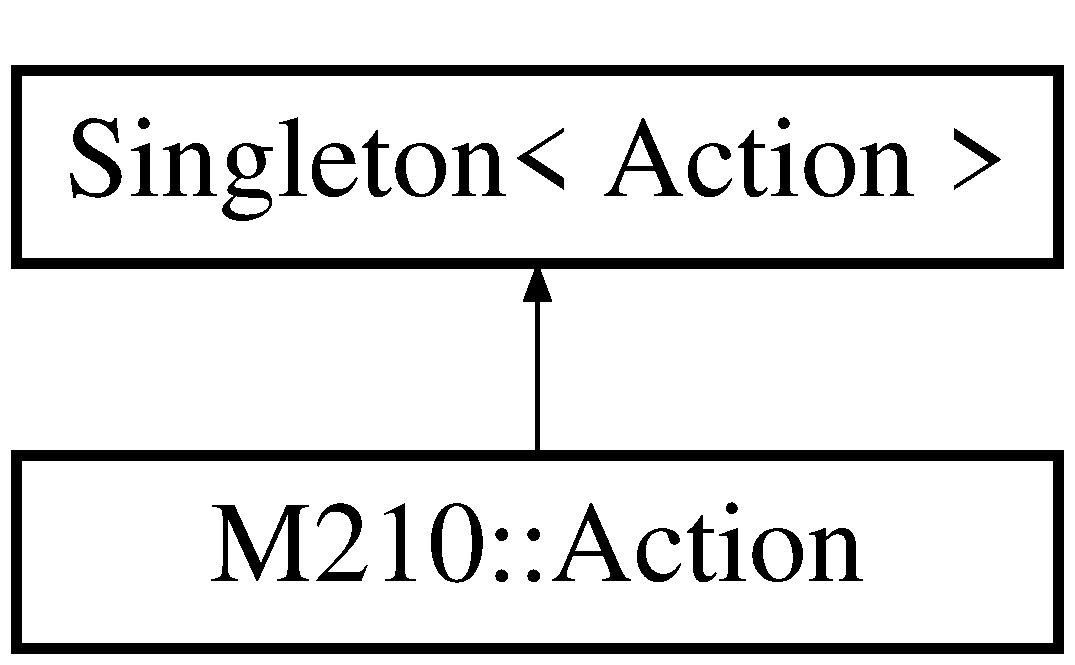
\includegraphics[height=2.000000cm]{class_m210_1_1_action}
\end{center}
\end{figure}
\subsection*{Public Types}
\begin{DoxyCompactItemize}
\item 
enum \mbox{\hyperlink{class_m210_1_1_action_ad9730775da7e3f099bef4571100e2f5d}{Mission\+Type}} \{ \mbox{\hyperlink{class_m210_1_1_action_ad9730775da7e3f099bef4571100e2f5da2c44c9af44f0d97e16ee0f7c0562658f}{V\+E\+L\+O\+C\+I\+TY}} = 1, 
{\bfseries P\+O\+S\+I\+T\+I\+ON}, 
{\bfseries P\+O\+S\+I\+T\+I\+O\+N\+\_\+\+O\+F\+F\+S\+ET}, 
{\bfseries W\+A\+Y\+P\+O\+I\+N\+TS}
 \}
\item 
enum \mbox{\hyperlink{class_m210_1_1_action_a0bb36f0932c930e1193428e3c3c98046}{Mission\+Action}} \{ \newline
\mbox{\hyperlink{class_m210_1_1_action_a0bb36f0932c930e1193428e3c3c98046ae9c51def583033613d398c85a26e927a}{S\+T\+A\+RT}} = 1, 
{\bfseries A\+DD}, 
{\bfseries R\+E\+S\+ET}, 
{\bfseries S\+T\+OP}, 
\newline
{\bfseries P\+A\+U\+SE}, 
{\bfseries R\+E\+S\+U\+ME}
 \}
\end{DoxyCompactItemize}
\subsection*{Public Member Functions}
\begin{DoxyCompactItemize}
\item 
\mbox{\hyperlink{class_m210_1_1_action_a4f457ccfc8336b565cadca56b36e0271}{Action}} ()
\item 
\mbox{\hyperlink{class_m210_1_1_action_acdb06775d157339256a8ecd55749226c}{$\sim$\+Action}} ()
\item 
void \mbox{\hyperlink{class_m210_1_1_action_a2079c96a8a88d045037c730f3f752d25}{set\+Flight\+Controller}} (\mbox{\hyperlink{class_m210_1_1_flight_controller}{Flight\+Controller}} $\ast$flight\+Controller)
\item 
bool \mbox{\hyperlink{class_m210_1_1_action_abd7130a46d5212979903418a0888aab5}{add}} (const \mbox{\hyperlink{class_m210_1_1_action_data}{Action\+Data}} $\ast$action\+Data)
\item 
void \mbox{\hyperlink{class_m210_1_1_action_a38eac84b9b832225548d16d37b16ffbd}{process}} () const
\end{DoxyCompactItemize}
\subsection*{Static Public Member Functions}
\begin{DoxyCompactItemize}
\item 
static void \mbox{\hyperlink{class_m210_1_1_action_ac60580623e0519acbada490342fc8f0b}{unit\+Test}} ()
\end{DoxyCompactItemize}


\subsection{Member Enumeration Documentation}
\mbox{\Hypertarget{class_m210_1_1_action_a0bb36f0932c930e1193428e3c3c98046}\label{class_m210_1_1_action_a0bb36f0932c930e1193428e3c3c98046}} 
\index{M210\+::\+Action@{M210\+::\+Action}!Mission\+Action@{Mission\+Action}}
\index{Mission\+Action@{Mission\+Action}!M210\+::\+Action@{M210\+::\+Action}}
\subsubsection{\texorpdfstring{Mission\+Action}{MissionAction}}
{\footnotesize\ttfamily enum \mbox{\hyperlink{class_m210_1_1_action_a0bb36f0932c930e1193428e3c3c98046}{M210\+::\+Action\+::\+Mission\+Action}}}

\begin{DoxyEnumFields}{Enumerator}
\raisebox{\heightof{T}}[0pt][0pt]{\index{S\+T\+A\+RT@{S\+T\+A\+RT}!M210\+::\+Action@{M210\+::\+Action}}\index{M210\+::\+Action@{M210\+::\+Action}!S\+T\+A\+RT@{S\+T\+A\+RT}}}\mbox{\Hypertarget{class_m210_1_1_action_a0bb36f0932c930e1193428e3c3c98046ae9c51def583033613d398c85a26e927a}\label{class_m210_1_1_action_a0bb36f0932c930e1193428e3c3c98046ae9c51def583033613d398c85a26e927a}} 
S\+T\+A\+RT&Mission action, mainly used with waypoints actions \\
\hline

\end{DoxyEnumFields}
\mbox{\Hypertarget{class_m210_1_1_action_ad9730775da7e3f099bef4571100e2f5d}\label{class_m210_1_1_action_ad9730775da7e3f099bef4571100e2f5d}} 
\index{M210\+::\+Action@{M210\+::\+Action}!Mission\+Type@{Mission\+Type}}
\index{Mission\+Type@{Mission\+Type}!M210\+::\+Action@{M210\+::\+Action}}
\subsubsection{\texorpdfstring{Mission\+Type}{MissionType}}
{\footnotesize\ttfamily enum \mbox{\hyperlink{class_m210_1_1_action_ad9730775da7e3f099bef4571100e2f5d}{M210\+::\+Action\+::\+Mission\+Type}}}

\begin{DoxyEnumFields}{Enumerator}
\raisebox{\heightof{T}}[0pt][0pt]{\index{V\+E\+L\+O\+C\+I\+TY@{V\+E\+L\+O\+C\+I\+TY}!M210\+::\+Action@{M210\+::\+Action}}\index{M210\+::\+Action@{M210\+::\+Action}!V\+E\+L\+O\+C\+I\+TY@{V\+E\+L\+O\+C\+I\+TY}}}\mbox{\Hypertarget{class_m210_1_1_action_ad9730775da7e3f099bef4571100e2f5da2c44c9af44f0d97e16ee0f7c0562658f}\label{class_m210_1_1_action_ad9730775da7e3f099bef4571100e2f5da2c44c9af44f0d97e16ee0f7c0562658f}} 
V\+E\+L\+O\+C\+I\+TY&Mission type, used when action concern a mission \\
\hline

\end{DoxyEnumFields}


\subsection{Constructor \& Destructor Documentation}
\mbox{\Hypertarget{class_m210_1_1_action_a4f457ccfc8336b565cadca56b36e0271}\label{class_m210_1_1_action_a4f457ccfc8336b565cadca56b36e0271}} 
\index{M210\+::\+Action@{M210\+::\+Action}!Action@{Action}}
\index{Action@{Action}!M210\+::\+Action@{M210\+::\+Action}}
\subsubsection{\texorpdfstring{Action()}{Action()}}
{\footnotesize\ttfamily Action\+::\+Action (\begin{DoxyParamCaption}{ }\end{DoxyParamCaption})}

Initialize action queue \mbox{\Hypertarget{class_m210_1_1_action_acdb06775d157339256a8ecd55749226c}\label{class_m210_1_1_action_acdb06775d157339256a8ecd55749226c}} 
\index{M210\+::\+Action@{M210\+::\+Action}!````~Action@{$\sim$\+Action}}
\index{````~Action@{$\sim$\+Action}!M210\+::\+Action@{M210\+::\+Action}}
\subsubsection{\texorpdfstring{$\sim$\+Action()}{~Action()}}
{\footnotesize\ttfamily Action\+::$\sim$\+Action (\begin{DoxyParamCaption}{ }\end{DoxyParamCaption})}

Close action queue and unlink it. 

\subsection{Member Function Documentation}
\mbox{\Hypertarget{class_m210_1_1_action_abd7130a46d5212979903418a0888aab5}\label{class_m210_1_1_action_abd7130a46d5212979903418a0888aab5}} 
\index{M210\+::\+Action@{M210\+::\+Action}!add@{add}}
\index{add@{add}!M210\+::\+Action@{M210\+::\+Action}}
\subsubsection{\texorpdfstring{add()}{add()}}
{\footnotesize\ttfamily bool Action\+::add (\begin{DoxyParamCaption}\item[{const \mbox{\hyperlink{class_m210_1_1_action_data}{Action\+Data}} $\ast$}]{action\+Data }\end{DoxyParamCaption})}

Add action data to queue 
\begin{DoxyParams}{Parameters}
{\em action\+Data} & Pointer to \mbox{\hyperlink{class_m210_1_1_action_data}{Action\+Data}} object to add \\
\hline
\end{DoxyParams}
\begin{DoxyReturn}{Returns}
true if action data has been added to queue, false otherwise 
\end{DoxyReturn}
\mbox{\Hypertarget{class_m210_1_1_action_a38eac84b9b832225548d16d37b16ffbd}\label{class_m210_1_1_action_a38eac84b9b832225548d16d37b16ffbd}} 
\index{M210\+::\+Action@{M210\+::\+Action}!process@{process}}
\index{process@{process}!M210\+::\+Action@{M210\+::\+Action}}
\subsubsection{\texorpdfstring{process()}{process()}}
{\footnotesize\ttfamily void Action\+::process (\begin{DoxyParamCaption}{ }\end{DoxyParamCaption}) const}

Receive message from queue a process it. Blocking call. \mbox{\Hypertarget{class_m210_1_1_action_a2079c96a8a88d045037c730f3f752d25}\label{class_m210_1_1_action_a2079c96a8a88d045037c730f3f752d25}} 
\index{M210\+::\+Action@{M210\+::\+Action}!set\+Flight\+Controller@{set\+Flight\+Controller}}
\index{set\+Flight\+Controller@{set\+Flight\+Controller}!M210\+::\+Action@{M210\+::\+Action}}
\subsubsection{\texorpdfstring{set\+Flight\+Controller()}{setFlightController()}}
{\footnotesize\ttfamily void M210\+::\+Action\+::set\+Flight\+Controller (\begin{DoxyParamCaption}\item[{\mbox{\hyperlink{class_m210_1_1_flight_controller}{Flight\+Controller}} $\ast$}]{flight\+Controller }\end{DoxyParamCaption})\hspace{0.3cm}{\ttfamily [inline]}}

Define the \mbox{\hyperlink{class_m210_1_1_flight_controller}{Flight\+Controller}} to whom the action should be transmitted 
\begin{DoxyParams}{Parameters}
{\em flight\+Controller} & Pointer to used \mbox{\hyperlink{class_m210_1_1_flight_controller}{Flight\+Controller}} \\
\hline
\end{DoxyParams}
\mbox{\Hypertarget{class_m210_1_1_action_ac60580623e0519acbada490342fc8f0b}\label{class_m210_1_1_action_ac60580623e0519acbada490342fc8f0b}} 
\index{M210\+::\+Action@{M210\+::\+Action}!unit\+Test@{unit\+Test}}
\index{unit\+Test@{unit\+Test}!M210\+::\+Action@{M210\+::\+Action}}
\subsubsection{\texorpdfstring{unit\+Test()}{unitTest()}}
{\footnotesize\ttfamily void Action\+::unit\+Test (\begin{DoxyParamCaption}{ }\end{DoxyParamCaption})\hspace{0.3cm}{\ttfamily [static]}}

Unit test to check that class is working. Called at the beginning of the program. Assert if a test fails 

The documentation for this class was generated from the following files\+:\begin{DoxyCompactItemize}
\item 
Action/\mbox{\hyperlink{_action_8h}{Action.\+h}}\item 
Action/\mbox{\hyperlink{_action_8cpp}{Action.\+cpp}}\end{DoxyCompactItemize}

\hypertarget{class_m210_1_1_action_data}{}\section{M210\+:\+:Action\+Data Class Reference}
\label{class_m210_1_1_action_data}\index{M210\+::\+Action\+Data@{M210\+::\+Action\+Data}}
\subsection*{Public Types}
\begin{DoxyCompactItemize}
\item 
enum \mbox{\hyperlink{class_m210_1_1_action_data_a35cd47f396d015ad523e845ddfaeab4c}{Action\+Id}} \{ \newline
\mbox{\hyperlink{class_m210_1_1_action_data_a35cd47f396d015ad523e845ddfaeab4ca2db55758ab72814e1383f5930fe6634a}{take\+Off}}, 
{\bfseries landing}, 
{\bfseries mission}, 
{\bfseries send\+Data\+To\+M\+S\+DK}, 
\newline
{\bfseries stop\+Aircraft}, 
{\bfseries emergency\+Stop}, 
{\bfseries emergency\+Release}, 
{\bfseries watchdog}, 
\newline
{\bfseries obtain\+Control\+Authority}, 
{\bfseries hello\+World}
 \}
\end{DoxyCompactItemize}
\subsection*{Public Member Functions}
\begin{DoxyCompactItemize}
\item 
\mbox{\hyperlink{class_m210_1_1_action_data_ad6cfcb4e00155902b01e889c189fec0d}{Action\+Data}} (\mbox{\hyperlink{class_m210_1_1_action_data_a35cd47f396d015ad523e845ddfaeab4c}{Action\+Id}} action\+Id, size\+\_\+t size=0)
\item 
\mbox{\hyperlink{class_m210_1_1_action_data_a5ecfc6f8a7f284d5430e9a59bbe399b7}{$\sim$\+Action\+Data}} ()
\item 
\mbox{\hyperlink{class_m210_1_1_action_data_a35cd47f396d015ad523e845ddfaeab4c}{Action\+Id}} \mbox{\hyperlink{class_m210_1_1_action_data_a9fff91f297d917c9519f3b4d2d2e130b}{get\+Action\+Id}} () const
\item 
bool \mbox{\hyperlink{class_m210_1_1_action_data_afc4ee6af4070e59d6753b85e150c0b88}{push}} (char c)
\item 
\mbox{\Hypertarget{class_m210_1_1_action_data_a805f85660b5dcde52f0008281980ae41}\label{class_m210_1_1_action_data_a805f85660b5dcde52f0008281980ae41}} 
bool {\bfseries push} (int i)
\item 
\mbox{\Hypertarget{class_m210_1_1_action_data_ae70334b31e84f40475efaa9d5e7fd856}\label{class_m210_1_1_action_data_ae70334b31e84f40475efaa9d5e7fd856}} 
bool {\bfseries push} (unsigned u)
\item 
\mbox{\Hypertarget{class_m210_1_1_action_data_ab26b540b0d6d1397a6fdd5d0c765d834}\label{class_m210_1_1_action_data_ab26b540b0d6d1397a6fdd5d0c765d834}} 
bool {\bfseries push} (float f)
\item 
\mbox{\Hypertarget{class_m210_1_1_action_data_a452788de9a3df42f2c71add388c6a42f}\label{class_m210_1_1_action_data_a452788de9a3df42f2c71add388c6a42f}} 
bool {\bfseries push} (const Telemetry\+::\+Vector3f \&v)
\item 
\mbox{\Hypertarget{class_m210_1_1_action_data_a1be77c54720d9d22ffb9d4019575405f}\label{class_m210_1_1_action_data_a1be77c54720d9d22ffb9d4019575405f}} 
bool {\bfseries push} (const uint8\+\_\+t $\ast$data, size\+\_\+t length)
\item 
bool \mbox{\hyperlink{class_m210_1_1_action_data_a590c1f07f361ace0bdf6072abec3cf48}{pop\+Char}} (char \&c)
\item 
\mbox{\Hypertarget{class_m210_1_1_action_data_a63d416b7fb36410d190d18a0203f715c}\label{class_m210_1_1_action_data_a63d416b7fb36410d190d18a0203f715c}} 
bool {\bfseries pop\+Int} (int \&i)
\item 
\mbox{\Hypertarget{class_m210_1_1_action_data_a8e215d39d3057afeec1d4b7776066182}\label{class_m210_1_1_action_data_a8e215d39d3057afeec1d4b7776066182}} 
bool {\bfseries pop\+Unsigned} (unsigned \&u)
\item 
\mbox{\Hypertarget{class_m210_1_1_action_data_a6a280037c2241d17e53e05d1fa114b30}\label{class_m210_1_1_action_data_a6a280037c2241d17e53e05d1fa114b30}} 
bool {\bfseries pop\+Float} (float \&f)
\item 
\mbox{\Hypertarget{class_m210_1_1_action_data_a0606072003289b2a504e2f9d450bac60}\label{class_m210_1_1_action_data_a0606072003289b2a504e2f9d450bac60}} 
bool {\bfseries pop\+Vector3f} (Telemetry\+::\+Vector3f \&v)
\end{DoxyCompactItemize}
\subsection*{Static Public Member Functions}
\begin{DoxyCompactItemize}
\item 
static void \mbox{\hyperlink{class_m210_1_1_action_data_acf9043b5b953a5a0c837ae679c9ab0e5}{unit\+Test}} ()
\end{DoxyCompactItemize}


\subsection{Member Enumeration Documentation}
\mbox{\Hypertarget{class_m210_1_1_action_data_a35cd47f396d015ad523e845ddfaeab4c}\label{class_m210_1_1_action_data_a35cd47f396d015ad523e845ddfaeab4c}} 
\index{M210\+::\+Action\+Data@{M210\+::\+Action\+Data}!Action\+Id@{Action\+Id}}
\index{Action\+Id@{Action\+Id}!M210\+::\+Action\+Data@{M210\+::\+Action\+Data}}
\subsubsection{\texorpdfstring{Action\+Id}{ActionId}}
{\footnotesize\ttfamily enum \mbox{\hyperlink{class_m210_1_1_action_data_a35cd47f396d015ad523e845ddfaeab4c}{M210\+::\+Action\+Data\+::\+Action\+Id}}}

\begin{DoxyEnumFields}{Enumerator}
\raisebox{\heightof{T}}[0pt][0pt]{\index{take\+Off@{take\+Off}!M210\+::\+Action\+Data@{M210\+::\+Action\+Data}}\index{M210\+::\+Action\+Data@{M210\+::\+Action\+Data}!take\+Off@{take\+Off}}}\mbox{\Hypertarget{class_m210_1_1_action_data_a35cd47f396d015ad523e845ddfaeab4ca2db55758ab72814e1383f5930fe6634a}\label{class_m210_1_1_action_data_a35cd47f396d015ad523e845ddfaeab4ca2db55758ab72814e1383f5930fe6634a}} 
take\+Off&Indicates which action is relative to current action data object \\
\hline

\end{DoxyEnumFields}


\subsection{Constructor \& Destructor Documentation}
\mbox{\Hypertarget{class_m210_1_1_action_data_ad6cfcb4e00155902b01e889c189fec0d}\label{class_m210_1_1_action_data_ad6cfcb4e00155902b01e889c189fec0d}} 
\index{M210\+::\+Action\+Data@{M210\+::\+Action\+Data}!Action\+Data@{Action\+Data}}
\index{Action\+Data@{Action\+Data}!M210\+::\+Action\+Data@{M210\+::\+Action\+Data}}
\subsubsection{\texorpdfstring{Action\+Data()}{ActionData()}}
{\footnotesize\ttfamily Action\+Data\+::\+Action\+Data (\begin{DoxyParamCaption}\item[{\mbox{\hyperlink{class_m210_1_1_action_data_a35cd47f396d015ad523e845ddfaeab4c}{Action\+Id}}}]{action\+Id,  }\item[{size\+\_\+t}]{size = {\ttfamily 0} }\end{DoxyParamCaption})\hspace{0.3cm}{\ttfamily [explicit]}}

Allocate dynamic memory for specified action 
\begin{DoxyParams}{Parameters}
{\em action\+Id} & \mbox{\hyperlink{class_m210_1_1_action}{Action}} id concerned by current action data \\
\hline
{\em size} & Size to allocate in dynamic memory \mbox{[}bytes\mbox{]} \\
\hline
\end{DoxyParams}
\mbox{\Hypertarget{class_m210_1_1_action_data_a5ecfc6f8a7f284d5430e9a59bbe399b7}\label{class_m210_1_1_action_data_a5ecfc6f8a7f284d5430e9a59bbe399b7}} 
\index{M210\+::\+Action\+Data@{M210\+::\+Action\+Data}!````~Action\+Data@{$\sim$\+Action\+Data}}
\index{````~Action\+Data@{$\sim$\+Action\+Data}!M210\+::\+Action\+Data@{M210\+::\+Action\+Data}}
\subsubsection{\texorpdfstring{$\sim$\+Action\+Data()}{~ActionData()}}
{\footnotesize\ttfamily Action\+Data\+::$\sim$\+Action\+Data (\begin{DoxyParamCaption}{ }\end{DoxyParamCaption})}

Delete dynamic memory allocated 

\subsection{Member Function Documentation}
\mbox{\Hypertarget{class_m210_1_1_action_data_a9fff91f297d917c9519f3b4d2d2e130b}\label{class_m210_1_1_action_data_a9fff91f297d917c9519f3b4d2d2e130b}} 
\index{M210\+::\+Action\+Data@{M210\+::\+Action\+Data}!get\+Action\+Id@{get\+Action\+Id}}
\index{get\+Action\+Id@{get\+Action\+Id}!M210\+::\+Action\+Data@{M210\+::\+Action\+Data}}
\subsubsection{\texorpdfstring{get\+Action\+Id()}{getActionId()}}
{\footnotesize\ttfamily \mbox{\hyperlink{class_m210_1_1_action_data_a35cd47f396d015ad523e845ddfaeab4c}{Action\+Id}} M210\+::\+Action\+Data\+::get\+Action\+Id (\begin{DoxyParamCaption}{ }\end{DoxyParamCaption}) const\hspace{0.3cm}{\ttfamily [inline]}}

Return action id concerned by current action data \begin{DoxyReturn}{Returns}
\mbox{\hyperlink{class_m210_1_1_action}{Action}} id 
\end{DoxyReturn}
\mbox{\Hypertarget{class_m210_1_1_action_data_a590c1f07f361ace0bdf6072abec3cf48}\label{class_m210_1_1_action_data_a590c1f07f361ace0bdf6072abec3cf48}} 
\index{M210\+::\+Action\+Data@{M210\+::\+Action\+Data}!pop\+Char@{pop\+Char}}
\index{pop\+Char@{pop\+Char}!M210\+::\+Action\+Data@{M210\+::\+Action\+Data}}
\subsubsection{\texorpdfstring{pop\+Char()}{popChar()}}
{\footnotesize\ttfamily bool Action\+Data\+::pop\+Char (\begin{DoxyParamCaption}\item[{char \&}]{c }\end{DoxyParamCaption})}

Dedicated pop methods See \mbox{\hyperlink{_action_data_8h_a4f0419f16d53bad043d5f85da427969d}{\+\_\+pop()}} macro for details 
\begin{DoxyParams}{Parameters}
{\em return} & variable \\
\hline
\end{DoxyParams}
\begin{DoxyReturn}{Returns}
False if there is no more data to read, true otherwise 
\end{DoxyReturn}
\mbox{\Hypertarget{class_m210_1_1_action_data_afc4ee6af4070e59d6753b85e150c0b88}\label{class_m210_1_1_action_data_afc4ee6af4070e59d6753b85e150c0b88}} 
\index{M210\+::\+Action\+Data@{M210\+::\+Action\+Data}!push@{push}}
\index{push@{push}!M210\+::\+Action\+Data@{M210\+::\+Action\+Data}}
\subsubsection{\texorpdfstring{push()}{push()}}
{\footnotesize\ttfamily bool Action\+Data\+::push (\begin{DoxyParamCaption}\item[{char}]{c }\end{DoxyParamCaption})}

Dedicated push methods See \mbox{\hyperlink{_action_data_8h_af32898bff77f8e81bd43ad0f30d25221}{\+\_\+push()}} macro for details 
\begin{DoxyParams}{Parameters}
{\em data} & to push \\
\hline
\end{DoxyParams}
\begin{DoxyReturn}{Returns}
False if there is not enough memory allocated, true otherwise 
\end{DoxyReturn}
\mbox{\Hypertarget{class_m210_1_1_action_data_acf9043b5b953a5a0c837ae679c9ab0e5}\label{class_m210_1_1_action_data_acf9043b5b953a5a0c837ae679c9ab0e5}} 
\index{M210\+::\+Action\+Data@{M210\+::\+Action\+Data}!unit\+Test@{unit\+Test}}
\index{unit\+Test@{unit\+Test}!M210\+::\+Action\+Data@{M210\+::\+Action\+Data}}
\subsubsection{\texorpdfstring{unit\+Test()}{unitTest()}}
{\footnotesize\ttfamily void Action\+Data\+::unit\+Test (\begin{DoxyParamCaption}{ }\end{DoxyParamCaption})\hspace{0.3cm}{\ttfamily [static]}}

Unit test to check that class is working. Called at the beginning of the program. Assert if a test fails 

The documentation for this class was generated from the following files\+:\begin{DoxyCompactItemize}
\item 
Action/\mbox{\hyperlink{_action_data_8h}{Action\+Data.\+h}}\item 
Action/\mbox{\hyperlink{_action_data_8cpp}{Action\+Data.\+cpp}}\end{DoxyCompactItemize}

\hypertarget{class_m210_1_1_avalanche_mission}{}\section{M210\+:\+:Avalanche\+Mission Class Reference}
\label{class_m210_1_1_avalanche_mission}\index{M210\+::\+Avalanche\+Mission@{M210\+::\+Avalanche\+Mission}}
\subsection*{Public Member Functions}
\begin{DoxyCompactItemize}
\item 
\mbox{\Hypertarget{class_m210_1_1_avalanche_mission_a11f7b825c70ca76e713e1397803dfea2}\label{class_m210_1_1_avalanche_mission_a11f7b825c70ca76e713e1397803dfea2}} 
void {\bfseries update\+Axis} (\mbox{\hyperlink{class_m210_1_1_geodetic_coord}{Geodetic\+Coord}} \&P1, \mbox{\hyperlink{class_m210_1_1_geodetic_coord}{Geodetic\+Coord}} \&P2)
\end{DoxyCompactItemize}


The documentation for this class was generated from the following files\+:\begin{DoxyCompactItemize}
\item 
Missions/\mbox{\hyperlink{_avalanche_mission_8h}{Avalanche\+Mission.\+h}}\item 
Missions/\mbox{\hyperlink{_avalanche_mission_8cpp}{Avalanche\+Mission.\+cpp}}\end{DoxyCompactItemize}

\hypertarget{class_m210_1_1_console}{}\section{M210\+:\+:Console Class Reference}
\label{class_m210_1_1_console}\index{M210\+::\+Console@{M210\+::\+Console}}
\subsection*{Public Member Functions}
\begin{DoxyCompactItemize}
\item 
\mbox{\hyperlink{class_m210_1_1_console_a144a023dffce3c666a3c7b160c6396e2}{Console}} (\mbox{\hyperlink{class_m210_1_1_flight_controller}{Flight\+Controller}} $\ast$flight\+Controller)
\item 
void \mbox{\hyperlink{class_m210_1_1_console_a46110349066e1bfb0ba274976da10a39}{launch\+Thread}} ()
\end{DoxyCompactItemize}


\subsection{Constructor \& Destructor Documentation}
\mbox{\Hypertarget{class_m210_1_1_console_a144a023dffce3c666a3c7b160c6396e2}\label{class_m210_1_1_console_a144a023dffce3c666a3c7b160c6396e2}} 
\index{M210\+::\+Console@{M210\+::\+Console}!Console@{Console}}
\index{Console@{Console}!M210\+::\+Console@{M210\+::\+Console}}
\subsubsection{\texorpdfstring{Console()}{Console()}}
{\footnotesize\ttfamily Console\+::\+Console (\begin{DoxyParamCaption}\item[{\mbox{\hyperlink{class_m210_1_1_flight_controller}{Flight\+Controller}} $\ast$}]{flight\+Controller }\end{DoxyParamCaption})\hspace{0.3cm}{\ttfamily [explicit]}}

Create console object 
\begin{DoxyParams}{Parameters}
{\em flight\+Controller} & \mbox{\hyperlink{class_m210_1_1_flight_controller}{Flight\+Controller}} to use \\
\hline
\end{DoxyParams}


\subsection{Member Function Documentation}
\mbox{\Hypertarget{class_m210_1_1_console_a46110349066e1bfb0ba274976da10a39}\label{class_m210_1_1_console_a46110349066e1bfb0ba274976da10a39}} 
\index{M210\+::\+Console@{M210\+::\+Console}!launch\+Thread@{launch\+Thread}}
\index{launch\+Thread@{launch\+Thread}!M210\+::\+Console@{M210\+::\+Console}}
\subsubsection{\texorpdfstring{launch\+Thread()}{launchThread()}}
{\footnotesize\ttfamily void Console\+::launch\+Thread (\begin{DoxyParamCaption}{ }\end{DoxyParamCaption})}

Create, set name and launch console thread 

The documentation for this class was generated from the following files\+:\begin{DoxyCompactItemize}
\item 
Communication/\mbox{\hyperlink{_console_8h}{Console.\+h}}\item 
Communication/\mbox{\hyperlink{_console_8cpp}{Console.\+cpp}}\end{DoxyCompactItemize}

\hypertarget{struct_m210_1_1_dms}{}\section{M210\+:\+:Dms Struct Reference}
\label{struct_m210_1_1_dms}\index{M210\+::\+Dms@{M210\+::\+Dms}}
\subsection*{Public Attributes}
\begin{DoxyCompactItemize}
\item 
int \mbox{\hyperlink{struct_m210_1_1_dms_a11468846637cfa06926a4e60d8fde581}{deg}}
\item 
\mbox{\Hypertarget{struct_m210_1_1_dms_a1a5fc2ae44e3f7d2d64ba6c5fd9b9a8d}\label{struct_m210_1_1_dms_a1a5fc2ae44e3f7d2d64ba6c5fd9b9a8d}} 
int {\bfseries min}
\item 
\mbox{\Hypertarget{struct_m210_1_1_dms_aea369ff322cefb83b6b9018de1750999}\label{struct_m210_1_1_dms_aea369ff322cefb83b6b9018de1750999}} 
double {\bfseries sec}
\end{DoxyCompactItemize}


\subsection{Member Data Documentation}
\mbox{\Hypertarget{struct_m210_1_1_dms_a11468846637cfa06926a4e60d8fde581}\label{struct_m210_1_1_dms_a11468846637cfa06926a4e60d8fde581}} 
\index{M210\+::\+Dms@{M210\+::\+Dms}!deg@{deg}}
\index{deg@{deg}!M210\+::\+Dms@{M210\+::\+Dms}}
\subsubsection{\texorpdfstring{deg}{deg}}
{\footnotesize\ttfamily int M210\+::\+Dms\+::deg}

$<$ Degree° minutes\textquotesingle{} seconds" notation 

The documentation for this struct was generated from the following file\+:\begin{DoxyCompactItemize}
\item 
Gps/\mbox{\hyperlink{_geodetic_coord_8h}{Geodetic\+Coord.\+h}}\end{DoxyCompactItemize}

\hypertarget{class_m210_1_1_emergency}{}\section{M210\+:\+:Emergency Class Reference}
\label{class_m210_1_1_emergency}\index{M210\+::\+Emergency@{M210\+::\+Emergency}}
\subsection*{Public Member Functions}
\begin{DoxyCompactItemize}
\item 
void \mbox{\hyperlink{class_m210_1_1_emergency_aa461736b60192940860a5f71839049b5}{set}} ()
\item 
void \mbox{\hyperlink{class_m210_1_1_emergency_a44add09d4d5016a54ffb714e468a40ac}{release}} ()
\item 
bool \mbox{\hyperlink{class_m210_1_1_emergency_a071e3eb6d67ee647b9d1aa9442f253e2}{is\+Enabled}} (bool display\+Error=false)
\end{DoxyCompactItemize}
\subsection*{Static Public Attributes}
\begin{DoxyCompactItemize}
\item 
\mbox{\Hypertarget{class_m210_1_1_emergency_a8282c33e7103d30584832fb20357e844}\label{class_m210_1_1_emergency_a8282c33e7103d30584832fb20357e844}} 
static const bool {\bfseries display\+Error} = true
\end{DoxyCompactItemize}


\subsection{Member Function Documentation}
\mbox{\Hypertarget{class_m210_1_1_emergency_a071e3eb6d67ee647b9d1aa9442f253e2}\label{class_m210_1_1_emergency_a071e3eb6d67ee647b9d1aa9442f253e2}} 
\index{M210\+::\+Emergency@{M210\+::\+Emergency}!is\+Enabled@{is\+Enabled}}
\index{is\+Enabled@{is\+Enabled}!M210\+::\+Emergency@{M210\+::\+Emergency}}
\subsubsection{\texorpdfstring{is\+Enabled()}{isEnabled()}}
{\footnotesize\ttfamily bool Emergency\+::is\+Enabled (\begin{DoxyParamCaption}\item[{bool}]{display\+Error = {\ttfamily false} }\end{DoxyParamCaption})}

Verify emergency state and display error message on first call (until emergency state is released) 
\begin{DoxyParams}{Parameters}
{\em display\+Error} & Force error message to be displayed. Use Emergency\+::display\+Error for a better readability \\
\hline
\end{DoxyParams}
\begin{DoxyReturn}{Returns}
True if emergency state is set 
\end{DoxyReturn}
\mbox{\Hypertarget{class_m210_1_1_emergency_a44add09d4d5016a54ffb714e468a40ac}\label{class_m210_1_1_emergency_a44add09d4d5016a54ffb714e468a40ac}} 
\index{M210\+::\+Emergency@{M210\+::\+Emergency}!release@{release}}
\index{release@{release}!M210\+::\+Emergency@{M210\+::\+Emergency}}
\subsubsection{\texorpdfstring{release()}{release()}}
{\footnotesize\ttfamily void Emergency\+::release (\begin{DoxyParamCaption}{ }\end{DoxyParamCaption})}

Release emergency state \mbox{\Hypertarget{class_m210_1_1_emergency_aa461736b60192940860a5f71839049b5}\label{class_m210_1_1_emergency_aa461736b60192940860a5f71839049b5}} 
\index{M210\+::\+Emergency@{M210\+::\+Emergency}!set@{set}}
\index{set@{set}!M210\+::\+Emergency@{M210\+::\+Emergency}}
\subsubsection{\texorpdfstring{set()}{set()}}
{\footnotesize\ttfamily void Emergency\+::set (\begin{DoxyParamCaption}{ }\end{DoxyParamCaption})}

Set emergency state 

The documentation for this class was generated from the following files\+:\begin{DoxyCompactItemize}
\item 
Aircraft/\mbox{\hyperlink{_emergency_8h}{Emergency.\+h}}\item 
Aircraft/\mbox{\hyperlink{_emergency_8cpp}{Emergency.\+cpp}}\end{DoxyCompactItemize}

\hypertarget{class_m210_1_1_flight_controller}{}\section{M210\+:\+:Flight\+Controller Class Reference}
\label{class_m210_1_1_flight_controller}\index{M210\+::\+Flight\+Controller@{M210\+::\+Flight\+Controller}}
\subsection*{Public Member Functions}
\begin{DoxyCompactItemize}
\item 
\mbox{\hyperlink{class_m210_1_1_flight_controller_a5094a2c6e0bb587cdc9bffabbad11551}{Flight\+Controller}} ()
\item 
\mbox{\hyperlink{class_m210_1_1_flight_controller_a9e78eb4ab3bea35b29a031b607a68c12}{$\sim$\+Flight\+Controller}} ()
\item 
void \mbox{\hyperlink{class_m210_1_1_flight_controller_ab8249276f7d2079bf8c363d92fec56de}{setup\+Vehicle}} (int argc, char $\ast$$\ast$argv)
\item 
void \mbox{\hyperlink{class_m210_1_1_flight_controller_a922010e478d2e6cca4432fd076c8a857}{obtain\+Ctrl\+Authority}} ()
\item 
void \mbox{\hyperlink{class_m210_1_1_flight_controller_afb8ae49d6b33d9e45b35b626cb51446a}{launch\+Flight\+Controller\+Thread}} ()
\item 
void \mbox{\hyperlink{class_m210_1_1_flight_controller_aa84f9729545c25d95efdf7d5b58fa635}{send\+Data\+To\+M\+S\+DK}} (const uint8\+\_\+t $\ast$data, size\+\_\+t length) const
\item 
bool \mbox{\hyperlink{class_m210_1_1_flight_controller_a543d0eeef65856bf15675707cd8fc9c7}{take\+Off}} ()
\item 
bool \mbox{\hyperlink{class_m210_1_1_flight_controller_a5ea1c7a5b70af967b0449a945e1758b9}{landing}} ()
\item 
void \mbox{\hyperlink{class_m210_1_1_flight_controller_a9d2685ace4ecff840505a37b348c6860}{move\+By\+Position}} (const Vector3f $\ast$offset, float yaw)
\item 
void \mbox{\hyperlink{class_m210_1_1_flight_controller_a7468154793bfd7dd6c1d2f19d0744ee1}{move\+By\+Velocity}} (const Vector3f $\ast$velocity, float yaw)
\item 
void \mbox{\hyperlink{class_m210_1_1_flight_controller_a3921aba5edb9b26e717fbbace6f837cd}{move\+By\+Position\+Offset}} (const Vector3f $\ast$offset, float yaw, float pos\+Threshold=0.\+2, float yaw\+Threshold=1.\+0)
\item 
void \mbox{\hyperlink{class_m210_1_1_flight_controller_a81fc1a9c9495f93ffebab36d4d574ea9}{waypoints\+Mission\+Action}} (unsigned task)
\item 
void \mbox{\hyperlink{class_m210_1_1_flight_controller_a60d0858a9cfd91bc362ec8b5b894d3b4}{stop\+Aircraft}} ()
\item 
void \mbox{\hyperlink{class_m210_1_1_flight_controller_a58dfd6c7a1777d8a2cd9820b9ce1763a}{emergency\+Stop}} ()
\item 
void \mbox{\hyperlink{class_m210_1_1_flight_controller_ae9bee302ab720de3436896e09b5a4d9e}{emergency\+Release}} ()
\item 
void \mbox{\hyperlink{class_m210_1_1_flight_controller_a0f1d22f6099140194df9639e04e458bb}{velocity\+And\+Yaw\+Rate\+Ctrl}} (const Vector3f $\ast$velocity, float yaw)
\item 
void \mbox{\hyperlink{class_m210_1_1_flight_controller_a664a1699471956c2caa80321dc4f3dfd}{position\+And\+Yaw\+Ctrl}} (const Vector3f $\ast$position, float yaw)
\item 
Vehicle $\ast$ \mbox{\hyperlink{class_m210_1_1_flight_controller_a3cb6f75de342d02a8856fff49c20c9d4}{get\+Vehicle}} () const
\item 
\mbox{\Hypertarget{class_m210_1_1_flight_controller_a5aa4c8f8c19a7772ef4718887667a38e}\label{class_m210_1_1_flight_controller_a5aa4c8f8c19a7772ef4718887667a38e}} 
S\+M\+State\+\_\+ {\bfseries get\+S\+M\+State} () const
\item 
\mbox{\Hypertarget{class_m210_1_1_flight_controller_ac66650cc3c68c4b319c801bfa38f7efc}\label{class_m210_1_1_flight_controller_ac66650cc3c68c4b319c801bfa38f7efc}} 
\mbox{\hyperlink{class_m210_1_1_watchdog}{Watchdog}} $\ast$ {\bfseries get\+Watchdog} () const
\item 
\mbox{\Hypertarget{class_m210_1_1_flight_controller_aaf7b6cfeb0f5e7bf200ea45feafec3a4}\label{class_m210_1_1_flight_controller_aaf7b6cfeb0f5e7bf200ea45feafec3a4}} 
void {\bfseries set\+S\+M\+State} (S\+M\+State\+\_\+ mode)
\end{DoxyCompactItemize}
\subsection*{Static Public Member Functions}
\begin{DoxyCompactItemize}
\item 
static bool \mbox{\hyperlink{class_m210_1_1_flight_controller_adc83a3c84c9472f0c2a62c1949cfdbfc}{start\+Global\+Position\+Broadcast}} (Vehicle $\ast$vehicle)
\end{DoxyCompactItemize}


\subsection{Constructor \& Destructor Documentation}
\mbox{\Hypertarget{class_m210_1_1_flight_controller_a5094a2c6e0bb587cdc9bffabbad11551}\label{class_m210_1_1_flight_controller_a5094a2c6e0bb587cdc9bffabbad11551}} 
\index{M210\+::\+Flight\+Controller@{M210\+::\+Flight\+Controller}!Flight\+Controller@{Flight\+Controller}}
\index{Flight\+Controller@{Flight\+Controller}!M210\+::\+Flight\+Controller@{M210\+::\+Flight\+Controller}}
\subsubsection{\texorpdfstring{Flight\+Controller()}{FlightController()}}
{\footnotesize\ttfamily Flight\+Controller\+::\+Flight\+Controller (\begin{DoxyParamCaption}{ }\end{DoxyParamCaption})}

Initialize flight controller and create mission \mbox{\Hypertarget{class_m210_1_1_flight_controller_a9e78eb4ab3bea35b29a031b607a68c12}\label{class_m210_1_1_flight_controller_a9e78eb4ab3bea35b29a031b607a68c12}} 
\index{M210\+::\+Flight\+Controller@{M210\+::\+Flight\+Controller}!````~Flight\+Controller@{$\sim$\+Flight\+Controller}}
\index{````~Flight\+Controller@{$\sim$\+Flight\+Controller}!M210\+::\+Flight\+Controller@{M210\+::\+Flight\+Controller}}
\subsubsection{\texorpdfstring{$\sim$\+Flight\+Controller()}{~FlightController()}}
{\footnotesize\ttfamily Flight\+Controller\+::$\sim$\+Flight\+Controller (\begin{DoxyParamCaption}{ }\end{DoxyParamCaption})}

Delete missions and flight controller attributes 

\subsection{Member Function Documentation}
\mbox{\Hypertarget{class_m210_1_1_flight_controller_ae9bee302ab720de3436896e09b5a4d9e}\label{class_m210_1_1_flight_controller_ae9bee302ab720de3436896e09b5a4d9e}} 
\index{M210\+::\+Flight\+Controller@{M210\+::\+Flight\+Controller}!emergency\+Release@{emergency\+Release}}
\index{emergency\+Release@{emergency\+Release}!M210\+::\+Flight\+Controller@{M210\+::\+Flight\+Controller}}
\subsubsection{\texorpdfstring{emergency\+Release()}{emergencyRelease()}}
{\footnotesize\ttfamily void Flight\+Controller\+::emergency\+Release (\begin{DoxyParamCaption}{ }\end{DoxyParamCaption})}

Reset flight controller emergency state \mbox{\Hypertarget{class_m210_1_1_flight_controller_a58dfd6c7a1777d8a2cd9820b9ce1763a}\label{class_m210_1_1_flight_controller_a58dfd6c7a1777d8a2cd9820b9ce1763a}} 
\index{M210\+::\+Flight\+Controller@{M210\+::\+Flight\+Controller}!emergency\+Stop@{emergency\+Stop}}
\index{emergency\+Stop@{emergency\+Stop}!M210\+::\+Flight\+Controller@{M210\+::\+Flight\+Controller}}
\subsubsection{\texorpdfstring{emergency\+Stop()}{emergencyStop()}}
{\footnotesize\ttfamily void Flight\+Controller\+::emergency\+Stop (\begin{DoxyParamCaption}{ }\end{DoxyParamCaption})}

Set flight controller emergency state and stop aircraft \mbox{\Hypertarget{class_m210_1_1_flight_controller_a3cb6f75de342d02a8856fff49c20c9d4}\label{class_m210_1_1_flight_controller_a3cb6f75de342d02a8856fff49c20c9d4}} 
\index{M210\+::\+Flight\+Controller@{M210\+::\+Flight\+Controller}!get\+Vehicle@{get\+Vehicle}}
\index{get\+Vehicle@{get\+Vehicle}!M210\+::\+Flight\+Controller@{M210\+::\+Flight\+Controller}}
\subsubsection{\texorpdfstring{get\+Vehicle()}{getVehicle()}}
{\footnotesize\ttfamily Vehicle$\ast$ M210\+::\+Flight\+Controller\+::get\+Vehicle (\begin{DoxyParamCaption}{ }\end{DoxyParamCaption}) const\hspace{0.3cm}{\ttfamily [inline]}}

Getters and setters functions \mbox{\Hypertarget{class_m210_1_1_flight_controller_a5ea1c7a5b70af967b0449a945e1758b9}\label{class_m210_1_1_flight_controller_a5ea1c7a5b70af967b0449a945e1758b9}} 
\index{M210\+::\+Flight\+Controller@{M210\+::\+Flight\+Controller}!landing@{landing}}
\index{landing@{landing}!M210\+::\+Flight\+Controller@{M210\+::\+Flight\+Controller}}
\subsubsection{\texorpdfstring{landing()}{landing()}}
{\footnotesize\ttfamily bool Flight\+Controller\+::landing (\begin{DoxyParamCaption}{ }\end{DoxyParamCaption})}

Monitored landing blocking call. \begin{DoxyReturn}{Returns}
True is landing success 
\end{DoxyReturn}
\mbox{\Hypertarget{class_m210_1_1_flight_controller_afb8ae49d6b33d9e45b35b626cb51446a}\label{class_m210_1_1_flight_controller_afb8ae49d6b33d9e45b35b626cb51446a}} 
\index{M210\+::\+Flight\+Controller@{M210\+::\+Flight\+Controller}!launch\+Flight\+Controller\+Thread@{launch\+Flight\+Controller\+Thread}}
\index{launch\+Flight\+Controller\+Thread@{launch\+Flight\+Controller\+Thread}!M210\+::\+Flight\+Controller@{M210\+::\+Flight\+Controller}}
\subsubsection{\texorpdfstring{launch\+Flight\+Controller\+Thread()}{launchFlightControllerThread()}}
{\footnotesize\ttfamily void Flight\+Controller\+::launch\+Flight\+Controller\+Thread (\begin{DoxyParamCaption}{ }\end{DoxyParamCaption})}

Launch flight controller thread \mbox{\Hypertarget{class_m210_1_1_flight_controller_a9d2685ace4ecff840505a37b348c6860}\label{class_m210_1_1_flight_controller_a9d2685ace4ecff840505a37b348c6860}} 
\index{M210\+::\+Flight\+Controller@{M210\+::\+Flight\+Controller}!move\+By\+Position@{move\+By\+Position}}
\index{move\+By\+Position@{move\+By\+Position}!M210\+::\+Flight\+Controller@{M210\+::\+Flight\+Controller}}
\subsubsection{\texorpdfstring{move\+By\+Position()}{moveByPosition()}}
{\footnotesize\ttfamily void Flight\+Controller\+::move\+By\+Position (\begin{DoxyParamCaption}\item[{const Vector3f $\ast$}]{offset,  }\item[{float}]{yaw }\end{DoxyParamCaption})}

Control the position and yaw angle of the vehicle. Here to try D\+JI S\+DK \mbox{\hyperlink{class_m210_1_1_flight_controller_a664a1699471956c2caa80321dc4f3dfd}{position\+And\+Yaw\+Ctrl()}} method To move aircraft of a desired offset please use \mbox{\hyperlink{class_m210_1_1_flight_controller_a3921aba5edb9b26e717fbbace6f837cd}{move\+By\+Position\+Offset()}} 
\begin{DoxyParams}{Parameters}
{\em offset} & Relative offset vector to move \mbox{[}m\mbox{]} Vector is relative to the ground x face to north, y face to east, z face to sky \\
\hline
{\em yaw} & Absolute yaw angle to set \mbox{[}deg\} \\
\hline
\end{DoxyParams}
\mbox{\Hypertarget{class_m210_1_1_flight_controller_a3921aba5edb9b26e717fbbace6f837cd}\label{class_m210_1_1_flight_controller_a3921aba5edb9b26e717fbbace6f837cd}} 
\index{M210\+::\+Flight\+Controller@{M210\+::\+Flight\+Controller}!move\+By\+Position\+Offset@{move\+By\+Position\+Offset}}
\index{move\+By\+Position\+Offset@{move\+By\+Position\+Offset}!M210\+::\+Flight\+Controller@{M210\+::\+Flight\+Controller}}
\subsubsection{\texorpdfstring{move\+By\+Position\+Offset()}{moveByPositionOffset()}}
{\footnotesize\ttfamily void Flight\+Controller\+::move\+By\+Position\+Offset (\begin{DoxyParamCaption}\item[{const Vector3f $\ast$}]{offset,  }\item[{float}]{yaw,  }\item[{float}]{pos\+Threshold = {\ttfamily 0.2},  }\item[{float}]{yaw\+Threshold = {\ttfamily 1.0} }\end{DoxyParamCaption})}

Position Control. Allows user to set an offset from current location. The aircraft will move to that position and stay there. 
\begin{DoxyParams}{Parameters}
{\em offset} & Relative offset vector to move \mbox{[}m\mbox{]} Vector is relative to the ground x face to north, y face to east, z face to sky \\
\hline
{\em yaw} & Absolute yaw angle to set \mbox{[}deg\mbox{]} \\
\hline
{\em pos\+Threshold} & Position threshold used by mission to consider position as reached \mbox{[}m\mbox{]} \\
\hline
{\em yaw\+Threshold} & Angle threshold used by mission to consider angle as reached \mbox{[}deg\mbox{]} \\
\hline
\end{DoxyParams}
\mbox{\Hypertarget{class_m210_1_1_flight_controller_a7468154793bfd7dd6c1d2f19d0744ee1}\label{class_m210_1_1_flight_controller_a7468154793bfd7dd6c1d2f19d0744ee1}} 
\index{M210\+::\+Flight\+Controller@{M210\+::\+Flight\+Controller}!move\+By\+Velocity@{move\+By\+Velocity}}
\index{move\+By\+Velocity@{move\+By\+Velocity}!M210\+::\+Flight\+Controller@{M210\+::\+Flight\+Controller}}
\subsubsection{\texorpdfstring{move\+By\+Velocity()}{moveByVelocity()}}
{\footnotesize\ttfamily void Flight\+Controller\+::move\+By\+Velocity (\begin{DoxyParamCaption}\item[{const Vector3f $\ast$}]{velocity,  }\item[{float}]{yaw }\end{DoxyParamCaption})}

Velocity Control. Allows user to set a velocity vector. The aircraft will move as described by vector until \mbox{\hyperlink{class_m210_1_1_flight_controller_a60d0858a9cfd91bc362ec8b5b894d3b4}{stop\+Aircraft()}} is called. 
\begin{DoxyParams}{Parameters}
{\em velocity} & Absolute velocity vector to set \mbox{[}m/s\mbox{]} Vector is relative to the ground x face to north, y face to east, z face to sky \\
\hline
{\em yaw} & Absolute yaw rate to set \mbox{[}deg/s\mbox{]} \\
\hline
\end{DoxyParams}
\mbox{\Hypertarget{class_m210_1_1_flight_controller_a922010e478d2e6cca4432fd076c8a857}\label{class_m210_1_1_flight_controller_a922010e478d2e6cca4432fd076c8a857}} 
\index{M210\+::\+Flight\+Controller@{M210\+::\+Flight\+Controller}!obtain\+Ctrl\+Authority@{obtain\+Ctrl\+Authority}}
\index{obtain\+Ctrl\+Authority@{obtain\+Ctrl\+Authority}!M210\+::\+Flight\+Controller@{M210\+::\+Flight\+Controller}}
\subsubsection{\texorpdfstring{obtain\+Ctrl\+Authority()}{obtainCtrlAuthority()}}
{\footnotesize\ttfamily void Flight\+Controller\+::obtain\+Ctrl\+Authority (\begin{DoxyParamCaption}{ }\end{DoxyParamCaption})}

Blocking call to obtain control authority \mbox{\Hypertarget{class_m210_1_1_flight_controller_a664a1699471956c2caa80321dc4f3dfd}\label{class_m210_1_1_flight_controller_a664a1699471956c2caa80321dc4f3dfd}} 
\index{M210\+::\+Flight\+Controller@{M210\+::\+Flight\+Controller}!position\+And\+Yaw\+Ctrl@{position\+And\+Yaw\+Ctrl}}
\index{position\+And\+Yaw\+Ctrl@{position\+And\+Yaw\+Ctrl}!M210\+::\+Flight\+Controller@{M210\+::\+Flight\+Controller}}
\subsubsection{\texorpdfstring{position\+And\+Yaw\+Ctrl()}{positionAndYawCtrl()}}
{\footnotesize\ttfamily void Flight\+Controller\+::position\+And\+Yaw\+Ctrl (\begin{DoxyParamCaption}\item[{const Vector3f $\ast$}]{position,  }\item[{float}]{yaw }\end{DoxyParamCaption})}

Control the position and yaw angle of the vehicle. On-\/board S\+DK method call with safety verification (emergency and watchdog states) This method must be used by all missions instead of direct call to vehicle method 
\begin{DoxyParams}{Parameters}
{\em position} & Relative position vector to move \mbox{[}m\mbox{]} Vector is relative to the ground x face to north, y face to east, z face to sky \\
\hline
{\em yaw} & Absolute yaw angle to set \mbox{[}deg\} \\
\hline
\end{DoxyParams}
\mbox{\Hypertarget{class_m210_1_1_flight_controller_aa84f9729545c25d95efdf7d5b58fa635}\label{class_m210_1_1_flight_controller_aa84f9729545c25d95efdf7d5b58fa635}} 
\index{M210\+::\+Flight\+Controller@{M210\+::\+Flight\+Controller}!send\+Data\+To\+M\+S\+DK@{send\+Data\+To\+M\+S\+DK}}
\index{send\+Data\+To\+M\+S\+DK@{send\+Data\+To\+M\+S\+DK}!M210\+::\+Flight\+Controller@{M210\+::\+Flight\+Controller}}
\subsubsection{\texorpdfstring{send\+Data\+To\+M\+S\+D\+K()}{sendDataToMSDK()}}
{\footnotesize\ttfamily void Flight\+Controller\+::send\+Data\+To\+M\+S\+DK (\begin{DoxyParamCaption}\item[{const uint8\+\_\+t $\ast$}]{data,  }\item[{size\+\_\+t}]{length }\end{DoxyParamCaption}) const}

Send data to mobile S\+DK 
\begin{DoxyParams}{Parameters}
{\em data} & Pointer to data to send \\
\hline
{\em length} & Length of data to send \\
\hline
\end{DoxyParams}
\mbox{\Hypertarget{class_m210_1_1_flight_controller_ab8249276f7d2079bf8c363d92fec56de}\label{class_m210_1_1_flight_controller_ab8249276f7d2079bf8c363d92fec56de}} 
\index{M210\+::\+Flight\+Controller@{M210\+::\+Flight\+Controller}!setup\+Vehicle@{setup\+Vehicle}}
\index{setup\+Vehicle@{setup\+Vehicle}!M210\+::\+Flight\+Controller@{M210\+::\+Flight\+Controller}}
\subsubsection{\texorpdfstring{setup\+Vehicle()}{setupVehicle()}}
{\footnotesize\ttfamily void Flight\+Controller\+::setup\+Vehicle (\begin{DoxyParamCaption}\item[{int}]{argc,  }\item[{char $\ast$$\ast$}]{argv }\end{DoxyParamCaption})}

Configure linux environment, get vehicle and obtain control authority 
\begin{DoxyParams}{Parameters}
{\em argc} & main parameter \\
\hline
{\em argv} & main parameter \\
\hline
\end{DoxyParams}
\mbox{\Hypertarget{class_m210_1_1_flight_controller_adc83a3c84c9472f0c2a62c1949cfdbfc}\label{class_m210_1_1_flight_controller_adc83a3c84c9472f0c2a62c1949cfdbfc}} 
\index{M210\+::\+Flight\+Controller@{M210\+::\+Flight\+Controller}!start\+Global\+Position\+Broadcast@{start\+Global\+Position\+Broadcast}}
\index{start\+Global\+Position\+Broadcast@{start\+Global\+Position\+Broadcast}!M210\+::\+Flight\+Controller@{M210\+::\+Flight\+Controller}}
\subsubsection{\texorpdfstring{start\+Global\+Position\+Broadcast()}{startGlobalPositionBroadcast()}}
{\footnotesize\ttfamily bool Flight\+Controller\+::start\+Global\+Position\+Broadcast (\begin{DoxyParamCaption}\item[{Vehicle $\ast$}]{vehicle }\end{DoxyParamCaption})\hspace{0.3cm}{\ttfamily [static]}}

Start broadcast send of position from aircaft 
\begin{DoxyParams}{Parameters}
{\em vehicle} & Vehicle concerned \\
\hline
\end{DoxyParams}
\begin{DoxyReturn}{Returns}
True if broadcast successfully started 
\end{DoxyReturn}
\mbox{\Hypertarget{class_m210_1_1_flight_controller_a60d0858a9cfd91bc362ec8b5b894d3b4}\label{class_m210_1_1_flight_controller_a60d0858a9cfd91bc362ec8b5b894d3b4}} 
\index{M210\+::\+Flight\+Controller@{M210\+::\+Flight\+Controller}!stop\+Aircraft@{stop\+Aircraft}}
\index{stop\+Aircraft@{stop\+Aircraft}!M210\+::\+Flight\+Controller@{M210\+::\+Flight\+Controller}}
\subsubsection{\texorpdfstring{stop\+Aircraft()}{stopAircraft()}}
{\footnotesize\ttfamily void Flight\+Controller\+::stop\+Aircraft (\begin{DoxyParamCaption}{ }\end{DoxyParamCaption})}

Stop aircraft Stop flight controller state machine and stop all current missions \mbox{\Hypertarget{class_m210_1_1_flight_controller_a543d0eeef65856bf15675707cd8fc9c7}\label{class_m210_1_1_flight_controller_a543d0eeef65856bf15675707cd8fc9c7}} 
\index{M210\+::\+Flight\+Controller@{M210\+::\+Flight\+Controller}!take\+Off@{take\+Off}}
\index{take\+Off@{take\+Off}!M210\+::\+Flight\+Controller@{M210\+::\+Flight\+Controller}}
\subsubsection{\texorpdfstring{take\+Off()}{takeOff()}}
{\footnotesize\ttfamily bool Flight\+Controller\+::take\+Off (\begin{DoxyParamCaption}{ }\end{DoxyParamCaption})}

Monitored take-\/off blocking call \begin{DoxyReturn}{Returns}
True if take-\/off success 
\end{DoxyReturn}
\mbox{\Hypertarget{class_m210_1_1_flight_controller_a0f1d22f6099140194df9639e04e458bb}\label{class_m210_1_1_flight_controller_a0f1d22f6099140194df9639e04e458bb}} 
\index{M210\+::\+Flight\+Controller@{M210\+::\+Flight\+Controller}!velocity\+And\+Yaw\+Rate\+Ctrl@{velocity\+And\+Yaw\+Rate\+Ctrl}}
\index{velocity\+And\+Yaw\+Rate\+Ctrl@{velocity\+And\+Yaw\+Rate\+Ctrl}!M210\+::\+Flight\+Controller@{M210\+::\+Flight\+Controller}}
\subsubsection{\texorpdfstring{velocity\+And\+Yaw\+Rate\+Ctrl()}{velocityAndYawRateCtrl()}}
{\footnotesize\ttfamily void Flight\+Controller\+::velocity\+And\+Yaw\+Rate\+Ctrl (\begin{DoxyParamCaption}\item[{const Vector3f $\ast$}]{velocity,  }\item[{float}]{yaw }\end{DoxyParamCaption})}

Control the velocity and yaw rate of the aircraft On-\/board S\+DK method call with safety verification (emergency and watchdog states) This method must be used by all missions instead of direct call to vehicle method 
\begin{DoxyParams}{Parameters}
{\em velocity} & Absolute velocity vector to set \mbox{[}m/s\mbox{]} Vector is relative to the ground x face to north, y face to east, z face to sky \\
\hline
{\em yaw} & Absolute yaw rate to set \mbox{[}deg/s\mbox{]} \\
\hline
\end{DoxyParams}
\mbox{\Hypertarget{class_m210_1_1_flight_controller_a81fc1a9c9495f93ffebab36d4d574ea9}\label{class_m210_1_1_flight_controller_a81fc1a9c9495f93ffebab36d4d574ea9}} 
\index{M210\+::\+Flight\+Controller@{M210\+::\+Flight\+Controller}!waypoints\+Mission\+Action@{waypoints\+Mission\+Action}}
\index{waypoints\+Mission\+Action@{waypoints\+Mission\+Action}!M210\+::\+Flight\+Controller@{M210\+::\+Flight\+Controller}}
\subsubsection{\texorpdfstring{waypoints\+Mission\+Action()}{waypointsMissionAction()}}
{\footnotesize\ttfamily void Flight\+Controller\+::waypoints\+Mission\+Action (\begin{DoxyParamCaption}\item[{unsigned}]{task }\end{DoxyParamCaption})}

Modify action flow of the waypoints mission 
\begin{DoxyParams}{Parameters}
{\em task} & Task to do, value of \mbox{\hyperlink{class_m210_1_1_action_a0bb36f0932c930e1193428e3c3c98046}{Action\+::\+Mission\+Action}} (\mbox{\hyperlink{_action_8h}{Action.\+h}}) structure \\
\hline
\end{DoxyParams}


The documentation for this class was generated from the following files\+:\begin{DoxyCompactItemize}
\item 
Aircraft/\mbox{\hyperlink{_flight_controller_8h}{Flight\+Controller.\+h}}\item 
Aircraft/\mbox{\hyperlink{_flight_controller_8cpp}{Flight\+Controller.\+cpp}}\end{DoxyCompactItemize}

\hypertarget{class_m210_1_1_geodetic_coord}{}\section{M210\+:\+:Geodetic\+Coord Class Reference}
\label{class_m210_1_1_geodetic_coord}\index{M210\+::\+Geodetic\+Coord@{M210\+::\+Geodetic\+Coord}}
\subsection*{Public Member Functions}
\begin{DoxyCompactItemize}
\item 
\mbox{\Hypertarget{class_m210_1_1_geodetic_coord_aa2a09cf073856b5f4411926ee1e8ddbc}\label{class_m210_1_1_geodetic_coord_aa2a09cf073856b5f4411926ee1e8ddbc}} 
{\bfseries Geodetic\+Coord} (double latitude, double longitude)
\item 
void \mbox{\hyperlink{class_m210_1_1_geodetic_coord_a5786ede63ff5e1ce58f56f76c1f183c1}{set\+From\+Rad}} (double lat, double lon)
\item 
void \mbox{\hyperlink{class_m210_1_1_geodetic_coord_a701bb7be9dcf1dc15e0bb3563e4f5470}{set\+From\+Deg}} (double lat, double lon)
\item 
void \mbox{\hyperlink{class_m210_1_1_geodetic_coord_a90974b429e6d1b7392998d56e934199c}{set\+From\+Dms}} (\mbox{\hyperlink{struct_m210_1_1_dms}{Dms}} $\ast$lat, \mbox{\hyperlink{struct_m210_1_1_dms}{Dms}} $\ast$lon)
\item 
void \mbox{\hyperlink{class_m210_1_1_geodetic_coord_aaa31d62bc5a256454057f0beef807e30}{set}} (\mbox{\hyperlink{class_m210_1_1_geodetic_coord}{Geodetic\+Coord}} \&p)
\item 
void \mbox{\hyperlink{class_m210_1_1_geodetic_coord_a91f14ba9099dba8ea3b6044d74663525}{dms}} (\mbox{\hyperlink{struct_m210_1_1_dms}{Dms}} \&lat, \mbox{\hyperlink{struct_m210_1_1_dms}{Dms}} \&lon) const
\item 
\mbox{\hyperlink{struct_m210_1_1_dms}{Dms}} \mbox{\hyperlink{class_m210_1_1_geodetic_coord_aed72a7b5422dbcdfe84a3168364cc4c0}{longitude\+Dms}} () const
\item 
\mbox{\hyperlink{struct_m210_1_1_dms}{Dms}} \mbox{\hyperlink{class_m210_1_1_geodetic_coord_ac55715a3e4b46492ec8c2fe497bcd1c0}{latitude\+Dms}} () const
\item 
double \mbox{\hyperlink{class_m210_1_1_geodetic_coord_a8ba9a63a7d067d52c9745ce6d20c7ec8}{longitude\+Rad}} () const
\item 
double \mbox{\hyperlink{class_m210_1_1_geodetic_coord_aaeb0aa298f82f3c8c122be133f2cedf3}{latitude\+Rad}} () const
\item 
double \mbox{\hyperlink{class_m210_1_1_geodetic_coord_a015d828931c1e3bb05de39bdbe415af9}{longitude\+Deg}} () const
\item 
double \mbox{\hyperlink{class_m210_1_1_geodetic_coord_ad5ade40ea0085e303396ffaec259aec7}{latitude\+Deg}} () const
\item 
\mbox{\hyperlink{class_m210_1_1_geodetic_coord}{Geodetic\+Coord}} \mbox{\hyperlink{class_m210_1_1_geodetic_coord_a763b712e1d458ba213f03bc4f45c1862}{operator+}} (const \mbox{\hyperlink{struct_vector2}{Vector2}} \&vec)
\item 
\mbox{\hyperlink{class_m210_1_1_geodetic_coord}{Geodetic\+Coord}} \mbox{\hyperlink{class_m210_1_1_geodetic_coord_ab3e11a59306f739faedd8be52472d2c4}{operator-\/}} (const \mbox{\hyperlink{struct_vector2}{Vector2}} \&vec)
\item 
\mbox{\hyperlink{class_m210_1_1_geodetic_coord}{Geodetic\+Coord}} \mbox{\hyperlink{class_m210_1_1_geodetic_coord_acf1d0b551179adc795b70a6d17d16fe2}{operator+=}} (const \mbox{\hyperlink{struct_vector2}{Vector2}} \&vec)
\item 
\mbox{\hyperlink{class_m210_1_1_geodetic_coord}{Geodetic\+Coord}} \mbox{\hyperlink{class_m210_1_1_geodetic_coord_ab73b337cbae14719e288ad88dcfdefd4}{operator-\/=}} (const \mbox{\hyperlink{struct_vector2}{Vector2}} \&vec)
\end{DoxyCompactItemize}
\subsection*{Static Public Member Functions}
\begin{DoxyCompactItemize}
\item 
static void \mbox{\hyperlink{class_m210_1_1_geodetic_coord_ab3ec669f7868af7901701dc6a615147e}{unit\+Test}} ()
\end{DoxyCompactItemize}


\subsection{Member Function Documentation}
\mbox{\Hypertarget{class_m210_1_1_geodetic_coord_a91f14ba9099dba8ea3b6044d74663525}\label{class_m210_1_1_geodetic_coord_a91f14ba9099dba8ea3b6044d74663525}} 
\index{M210\+::\+Geodetic\+Coord@{M210\+::\+Geodetic\+Coord}!dms@{dms}}
\index{dms@{dms}!M210\+::\+Geodetic\+Coord@{M210\+::\+Geodetic\+Coord}}
\subsubsection{\texorpdfstring{dms()}{dms()}}
{\footnotesize\ttfamily void Geodetic\+Coord\+::dms (\begin{DoxyParamCaption}\item[{\mbox{\hyperlink{struct_m210_1_1_dms}{Dms}} \&}]{lat,  }\item[{\mbox{\hyperlink{struct_m210_1_1_dms}{Dms}} \&}]{lon }\end{DoxyParamCaption}) const}

Get current position 
\begin{DoxyParams}{Parameters}
{\em lat} & \mbox{\hyperlink{struct_m210_1_1_dms}{Dms}} structure to store latitude \\
\hline
{\em lon} & \mbox{\hyperlink{struct_m210_1_1_dms}{Dms}} structure to store longitude \\
\hline
\end{DoxyParams}
\mbox{\Hypertarget{class_m210_1_1_geodetic_coord_ad5ade40ea0085e303396ffaec259aec7}\label{class_m210_1_1_geodetic_coord_ad5ade40ea0085e303396ffaec259aec7}} 
\index{M210\+::\+Geodetic\+Coord@{M210\+::\+Geodetic\+Coord}!latitude\+Deg@{latitude\+Deg}}
\index{latitude\+Deg@{latitude\+Deg}!M210\+::\+Geodetic\+Coord@{M210\+::\+Geodetic\+Coord}}
\subsubsection{\texorpdfstring{latitude\+Deg()}{latitudeDeg()}}
{\footnotesize\ttfamily double Geodetic\+Coord\+::latitude\+Deg (\begin{DoxyParamCaption}{ }\end{DoxyParamCaption}) const}

Get current latitude \begin{DoxyReturn}{Returns}
Latitude \mbox{[}deg\mbox{]} 
\end{DoxyReturn}
\mbox{\Hypertarget{class_m210_1_1_geodetic_coord_ac55715a3e4b46492ec8c2fe497bcd1c0}\label{class_m210_1_1_geodetic_coord_ac55715a3e4b46492ec8c2fe497bcd1c0}} 
\index{M210\+::\+Geodetic\+Coord@{M210\+::\+Geodetic\+Coord}!latitude\+Dms@{latitude\+Dms}}
\index{latitude\+Dms@{latitude\+Dms}!M210\+::\+Geodetic\+Coord@{M210\+::\+Geodetic\+Coord}}
\subsubsection{\texorpdfstring{latitude\+Dms()}{latitudeDms()}}
{\footnotesize\ttfamily \mbox{\hyperlink{struct_m210_1_1_dms}{Dms}} Geodetic\+Coord\+::latitude\+Dms (\begin{DoxyParamCaption}{ }\end{DoxyParamCaption}) const}

Get current latitude \begin{DoxyReturn}{Returns}
Latitude \mbox{[}\mbox{\hyperlink{struct_m210_1_1_dms}{Dms}}\} 
\end{DoxyReturn}
\mbox{\Hypertarget{class_m210_1_1_geodetic_coord_aaeb0aa298f82f3c8c122be133f2cedf3}\label{class_m210_1_1_geodetic_coord_aaeb0aa298f82f3c8c122be133f2cedf3}} 
\index{M210\+::\+Geodetic\+Coord@{M210\+::\+Geodetic\+Coord}!latitude\+Rad@{latitude\+Rad}}
\index{latitude\+Rad@{latitude\+Rad}!M210\+::\+Geodetic\+Coord@{M210\+::\+Geodetic\+Coord}}
\subsubsection{\texorpdfstring{latitude\+Rad()}{latitudeRad()}}
{\footnotesize\ttfamily double Geodetic\+Coord\+::latitude\+Rad (\begin{DoxyParamCaption}{ }\end{DoxyParamCaption}) const}

Get current latitude \begin{DoxyReturn}{Returns}
Latitude \mbox{[}rad\mbox{]} 
\end{DoxyReturn}
\mbox{\Hypertarget{class_m210_1_1_geodetic_coord_a015d828931c1e3bb05de39bdbe415af9}\label{class_m210_1_1_geodetic_coord_a015d828931c1e3bb05de39bdbe415af9}} 
\index{M210\+::\+Geodetic\+Coord@{M210\+::\+Geodetic\+Coord}!longitude\+Deg@{longitude\+Deg}}
\index{longitude\+Deg@{longitude\+Deg}!M210\+::\+Geodetic\+Coord@{M210\+::\+Geodetic\+Coord}}
\subsubsection{\texorpdfstring{longitude\+Deg()}{longitudeDeg()}}
{\footnotesize\ttfamily double Geodetic\+Coord\+::longitude\+Deg (\begin{DoxyParamCaption}{ }\end{DoxyParamCaption}) const}

Get current longitude \begin{DoxyReturn}{Returns}
Longitude \mbox{[}deg\mbox{]} 
\end{DoxyReturn}
\mbox{\Hypertarget{class_m210_1_1_geodetic_coord_aed72a7b5422dbcdfe84a3168364cc4c0}\label{class_m210_1_1_geodetic_coord_aed72a7b5422dbcdfe84a3168364cc4c0}} 
\index{M210\+::\+Geodetic\+Coord@{M210\+::\+Geodetic\+Coord}!longitude\+Dms@{longitude\+Dms}}
\index{longitude\+Dms@{longitude\+Dms}!M210\+::\+Geodetic\+Coord@{M210\+::\+Geodetic\+Coord}}
\subsubsection{\texorpdfstring{longitude\+Dms()}{longitudeDms()}}
{\footnotesize\ttfamily \mbox{\hyperlink{struct_m210_1_1_dms}{Dms}} Geodetic\+Coord\+::longitude\+Dms (\begin{DoxyParamCaption}{ }\end{DoxyParamCaption}) const}

Get current longitude \begin{DoxyReturn}{Returns}
Longitude \mbox{[}\mbox{\hyperlink{struct_m210_1_1_dms}{Dms}}\mbox{]} 
\end{DoxyReturn}
\mbox{\Hypertarget{class_m210_1_1_geodetic_coord_a8ba9a63a7d067d52c9745ce6d20c7ec8}\label{class_m210_1_1_geodetic_coord_a8ba9a63a7d067d52c9745ce6d20c7ec8}} 
\index{M210\+::\+Geodetic\+Coord@{M210\+::\+Geodetic\+Coord}!longitude\+Rad@{longitude\+Rad}}
\index{longitude\+Rad@{longitude\+Rad}!M210\+::\+Geodetic\+Coord@{M210\+::\+Geodetic\+Coord}}
\subsubsection{\texorpdfstring{longitude\+Rad()}{longitudeRad()}}
{\footnotesize\ttfamily double Geodetic\+Coord\+::longitude\+Rad (\begin{DoxyParamCaption}{ }\end{DoxyParamCaption}) const}

Get current longitude \begin{DoxyReturn}{Returns}
Longitude \mbox{[}rad\mbox{]} 
\end{DoxyReturn}
\mbox{\Hypertarget{class_m210_1_1_geodetic_coord_a763b712e1d458ba213f03bc4f45c1862}\label{class_m210_1_1_geodetic_coord_a763b712e1d458ba213f03bc4f45c1862}} 
\index{M210\+::\+Geodetic\+Coord@{M210\+::\+Geodetic\+Coord}!operator+@{operator+}}
\index{operator+@{operator+}!M210\+::\+Geodetic\+Coord@{M210\+::\+Geodetic\+Coord}}
\subsubsection{\texorpdfstring{operator+()}{operator+()}}
{\footnotesize\ttfamily \mbox{\hyperlink{class_m210_1_1_geodetic_coord}{Geodetic\+Coord}} Geodetic\+Coord\+::operator+ (\begin{DoxyParamCaption}\item[{const \mbox{\hyperlink{struct_vector2}{Vector2}} \&}]{vec }\end{DoxyParamCaption})}

Add a N\+ED vector to a geodetic position 
\begin{DoxyParams}{Parameters}
{\em vec} & Vector to add \mbox{[}m\mbox{]} \\
\hline
\end{DoxyParams}
\begin{DoxyReturn}{Returns}
Geodetic coordinates of the new point 
\end{DoxyReturn}
\mbox{\Hypertarget{class_m210_1_1_geodetic_coord_acf1d0b551179adc795b70a6d17d16fe2}\label{class_m210_1_1_geodetic_coord_acf1d0b551179adc795b70a6d17d16fe2}} 
\index{M210\+::\+Geodetic\+Coord@{M210\+::\+Geodetic\+Coord}!operator+=@{operator+=}}
\index{operator+=@{operator+=}!M210\+::\+Geodetic\+Coord@{M210\+::\+Geodetic\+Coord}}
\subsubsection{\texorpdfstring{operator+=()}{operator+=()}}
{\footnotesize\ttfamily \mbox{\hyperlink{class_m210_1_1_geodetic_coord}{Geodetic\+Coord}} Geodetic\+Coord\+::operator+= (\begin{DoxyParamCaption}\item[{const \mbox{\hyperlink{struct_vector2}{Vector2}} \&}]{vec }\end{DoxyParamCaption})}

Add a N\+ED vector to the current geodetic position 
\begin{DoxyParams}{Parameters}
{\em vec} & Vector to add \mbox{[}m\mbox{]} \\
\hline
\end{DoxyParams}
\begin{DoxyReturn}{Returns}
Current geodetic coordinates object 
\end{DoxyReturn}
\mbox{\Hypertarget{class_m210_1_1_geodetic_coord_ab3e11a59306f739faedd8be52472d2c4}\label{class_m210_1_1_geodetic_coord_ab3e11a59306f739faedd8be52472d2c4}} 
\index{M210\+::\+Geodetic\+Coord@{M210\+::\+Geodetic\+Coord}!operator-\/@{operator-\/}}
\index{operator-\/@{operator-\/}!M210\+::\+Geodetic\+Coord@{M210\+::\+Geodetic\+Coord}}
\subsubsection{\texorpdfstring{operator-\/()}{operator-()}}
{\footnotesize\ttfamily \mbox{\hyperlink{class_m210_1_1_geodetic_coord}{Geodetic\+Coord}} Geodetic\+Coord\+::operator-\/ (\begin{DoxyParamCaption}\item[{const \mbox{\hyperlink{struct_vector2}{Vector2}} \&}]{vec }\end{DoxyParamCaption})}

Subtract a N\+ED vector to a geodetic position 
\begin{DoxyParams}{Parameters}
{\em vec} & Vector to Subtract \mbox{[}m\mbox{]} \\
\hline
\end{DoxyParams}
\begin{DoxyReturn}{Returns}
Geodetic coordinates of the new point 
\end{DoxyReturn}
\mbox{\Hypertarget{class_m210_1_1_geodetic_coord_ab73b337cbae14719e288ad88dcfdefd4}\label{class_m210_1_1_geodetic_coord_ab73b337cbae14719e288ad88dcfdefd4}} 
\index{M210\+::\+Geodetic\+Coord@{M210\+::\+Geodetic\+Coord}!operator-\/=@{operator-\/=}}
\index{operator-\/=@{operator-\/=}!M210\+::\+Geodetic\+Coord@{M210\+::\+Geodetic\+Coord}}
\subsubsection{\texorpdfstring{operator-\/=()}{operator-=()}}
{\footnotesize\ttfamily \mbox{\hyperlink{class_m210_1_1_geodetic_coord}{Geodetic\+Coord}} Geodetic\+Coord\+::operator-\/= (\begin{DoxyParamCaption}\item[{const \mbox{\hyperlink{struct_vector2}{Vector2}} \&}]{vec }\end{DoxyParamCaption})}

Subtract a N\+ED vector to the current geodetic position 
\begin{DoxyParams}{Parameters}
{\em vec} & Vector to Subtract \mbox{[}m\mbox{]} \\
\hline
\end{DoxyParams}
\begin{DoxyReturn}{Returns}
Current geodetic coordinates object 
\end{DoxyReturn}
\mbox{\Hypertarget{class_m210_1_1_geodetic_coord_aaa31d62bc5a256454057f0beef807e30}\label{class_m210_1_1_geodetic_coord_aaa31d62bc5a256454057f0beef807e30}} 
\index{M210\+::\+Geodetic\+Coord@{M210\+::\+Geodetic\+Coord}!set@{set}}
\index{set@{set}!M210\+::\+Geodetic\+Coord@{M210\+::\+Geodetic\+Coord}}
\subsubsection{\texorpdfstring{set()}{set()}}
{\footnotesize\ttfamily void Geodetic\+Coord\+::set (\begin{DoxyParamCaption}\item[{\mbox{\hyperlink{class_m210_1_1_geodetic_coord}{Geodetic\+Coord}} \&}]{p }\end{DoxyParamCaption})}

Set current position from an other \mbox{\hyperlink{class_m210_1_1_geodetic_coord}{Geodetic\+Coord}} object 
\begin{DoxyParams}{Parameters}
{\em p} & Object whose position has to be copied \\
\hline
\end{DoxyParams}
\mbox{\Hypertarget{class_m210_1_1_geodetic_coord_a701bb7be9dcf1dc15e0bb3563e4f5470}\label{class_m210_1_1_geodetic_coord_a701bb7be9dcf1dc15e0bb3563e4f5470}} 
\index{M210\+::\+Geodetic\+Coord@{M210\+::\+Geodetic\+Coord}!set\+From\+Deg@{set\+From\+Deg}}
\index{set\+From\+Deg@{set\+From\+Deg}!M210\+::\+Geodetic\+Coord@{M210\+::\+Geodetic\+Coord}}
\subsubsection{\texorpdfstring{set\+From\+Deg()}{setFromDeg()}}
{\footnotesize\ttfamily void Geodetic\+Coord\+::set\+From\+Deg (\begin{DoxyParamCaption}\item[{double}]{lat,  }\item[{double}]{lon }\end{DoxyParamCaption})}

Set current position 
\begin{DoxyParams}{Parameters}
{\em lat} & Latitude \mbox{[}deg\mbox{]} \\
\hline
{\em lon} & Longitude \mbox{[}deg\mbox{]} \\
\hline
\end{DoxyParams}
\mbox{\Hypertarget{class_m210_1_1_geodetic_coord_a90974b429e6d1b7392998d56e934199c}\label{class_m210_1_1_geodetic_coord_a90974b429e6d1b7392998d56e934199c}} 
\index{M210\+::\+Geodetic\+Coord@{M210\+::\+Geodetic\+Coord}!set\+From\+Dms@{set\+From\+Dms}}
\index{set\+From\+Dms@{set\+From\+Dms}!M210\+::\+Geodetic\+Coord@{M210\+::\+Geodetic\+Coord}}
\subsubsection{\texorpdfstring{set\+From\+Dms()}{setFromDms()}}
{\footnotesize\ttfamily void Geodetic\+Coord\+::set\+From\+Dms (\begin{DoxyParamCaption}\item[{\mbox{\hyperlink{struct_m210_1_1_dms}{Dms}} $\ast$}]{lat,  }\item[{\mbox{\hyperlink{struct_m210_1_1_dms}{Dms}} $\ast$}]{lon }\end{DoxyParamCaption})}

Set current position 
\begin{DoxyParams}{Parameters}
{\em lat} & Latitude \mbox{[}\mbox{\hyperlink{struct_m210_1_1_dms}{Dms}}\mbox{]} \\
\hline
{\em lon} & Longitude \mbox{[}\mbox{\hyperlink{struct_m210_1_1_dms}{Dms}}\mbox{]} \\
\hline
\end{DoxyParams}
\mbox{\Hypertarget{class_m210_1_1_geodetic_coord_a5786ede63ff5e1ce58f56f76c1f183c1}\label{class_m210_1_1_geodetic_coord_a5786ede63ff5e1ce58f56f76c1f183c1}} 
\index{M210\+::\+Geodetic\+Coord@{M210\+::\+Geodetic\+Coord}!set\+From\+Rad@{set\+From\+Rad}}
\index{set\+From\+Rad@{set\+From\+Rad}!M210\+::\+Geodetic\+Coord@{M210\+::\+Geodetic\+Coord}}
\subsubsection{\texorpdfstring{set\+From\+Rad()}{setFromRad()}}
{\footnotesize\ttfamily void Geodetic\+Coord\+::set\+From\+Rad (\begin{DoxyParamCaption}\item[{double}]{lat,  }\item[{double}]{lon }\end{DoxyParamCaption})}

Set current position 
\begin{DoxyParams}{Parameters}
{\em lat} & Latitude \mbox{[}rad\mbox{]} \\
\hline
{\em lon} & Longitude \mbox{[}rad\mbox{]} \\
\hline
\end{DoxyParams}
\mbox{\Hypertarget{class_m210_1_1_geodetic_coord_ab3ec669f7868af7901701dc6a615147e}\label{class_m210_1_1_geodetic_coord_ab3ec669f7868af7901701dc6a615147e}} 
\index{M210\+::\+Geodetic\+Coord@{M210\+::\+Geodetic\+Coord}!unit\+Test@{unit\+Test}}
\index{unit\+Test@{unit\+Test}!M210\+::\+Geodetic\+Coord@{M210\+::\+Geodetic\+Coord}}
\subsubsection{\texorpdfstring{unit\+Test()}{unitTest()}}
{\footnotesize\ttfamily void Geodetic\+Coord\+::unit\+Test (\begin{DoxyParamCaption}{ }\end{DoxyParamCaption})\hspace{0.3cm}{\ttfamily [static]}}

Unit test to check that class is working. Called at the beginning of the program. Assert if a test fails 

The documentation for this class was generated from the following files\+:\begin{DoxyCompactItemize}
\item 
Gps/\mbox{\hyperlink{_geodetic_coord_8h}{Geodetic\+Coord.\+h}}\item 
Gps/\mbox{\hyperlink{_geodetic_coord_8cpp}{Geodetic\+Coord.\+cpp}}\end{DoxyCompactItemize}

\hypertarget{class_m210_1_1_gps_axis}{}\section{M210\+:\+:Gps\+Axis Class Reference}
\label{class_m210_1_1_gps_axis}\index{M210\+::\+Gps\+Axis@{M210\+::\+Gps\+Axis}}
Inheritance diagram for M210\+:\+:Gps\+Axis\+:\begin{figure}[H]
\begin{center}
\leavevmode
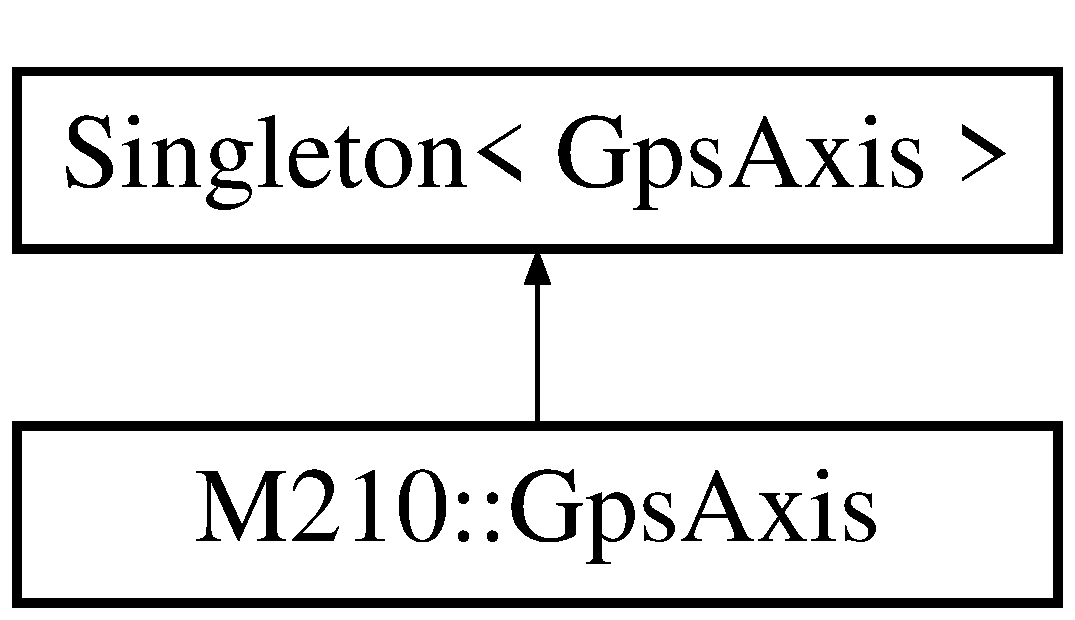
\includegraphics[height=2.000000cm]{class_m210_1_1_gps_axis}
\end{center}
\end{figure}
\subsection*{Public Member Functions}
\begin{DoxyCompactItemize}
\item 
void \mbox{\hyperlink{class_m210_1_1_gps_axis_ac926b543520abc8c87e3692a560954ad}{set\+Rotation\+Angle}} (double angle)
\item 
void \mbox{\hyperlink{class_m210_1_1_gps_axis_a89a2b85d3f6b644fd3b4836dcd69c88b}{update\+Front\+Vector}} (const \mbox{\hyperlink{struct_vector2}{Vector2}} \&v)
\item 
\mbox{\hyperlink{struct_vector2}{Vector2}} \mbox{\hyperlink{class_m210_1_1_gps_axis_a2ca6c7a8f723940b09d00441cff7d4a9}{project\+Vector}} (\mbox{\hyperlink{struct_vector2}{Vector2}} \&v) const
\item 
\mbox{\hyperlink{struct_vector2}{Vector2}} \mbox{\hyperlink{class_m210_1_1_gps_axis_afbcf2ad8d7c70a6e3422272a9abe4086}{revert\+Vector}} (\mbox{\hyperlink{struct_vector2}{Vector2}} \&v) const
\end{DoxyCompactItemize}


\subsection{Member Function Documentation}
\mbox{\Hypertarget{class_m210_1_1_gps_axis_a2ca6c7a8f723940b09d00441cff7d4a9}\label{class_m210_1_1_gps_axis_a2ca6c7a8f723940b09d00441cff7d4a9}} 
\index{M210\+::\+Gps\+Axis@{M210\+::\+Gps\+Axis}!project\+Vector@{project\+Vector}}
\index{project\+Vector@{project\+Vector}!M210\+::\+Gps\+Axis@{M210\+::\+Gps\+Axis}}
\subsubsection{\texorpdfstring{project\+Vector()}{projectVector()}}
{\footnotesize\ttfamily \mbox{\hyperlink{struct_vector2}{Vector2}} Gps\+Axis\+::project\+Vector (\begin{DoxyParamCaption}\item[{\mbox{\hyperlink{struct_vector2}{Vector2}} \&}]{v }\end{DoxyParamCaption}) const}

Project vector from custom base to N\+ED 
\begin{DoxyParams}{Parameters}
{\em v} & Vector to project \\
\hline
\end{DoxyParams}
\begin{DoxyReturn}{Returns}
Projected vector 
\end{DoxyReturn}
\mbox{\Hypertarget{class_m210_1_1_gps_axis_afbcf2ad8d7c70a6e3422272a9abe4086}\label{class_m210_1_1_gps_axis_afbcf2ad8d7c70a6e3422272a9abe4086}} 
\index{M210\+::\+Gps\+Axis@{M210\+::\+Gps\+Axis}!revert\+Vector@{revert\+Vector}}
\index{revert\+Vector@{revert\+Vector}!M210\+::\+Gps\+Axis@{M210\+::\+Gps\+Axis}}
\subsubsection{\texorpdfstring{revert\+Vector()}{revertVector()}}
{\footnotesize\ttfamily \mbox{\hyperlink{struct_vector2}{Vector2}} Gps\+Axis\+::revert\+Vector (\begin{DoxyParamCaption}\item[{\mbox{\hyperlink{struct_vector2}{Vector2}} \&}]{v }\end{DoxyParamCaption}) const}

Project vector from N\+ED to custom base 
\begin{DoxyParams}{Parameters}
{\em v} & Vector to project \\
\hline
\end{DoxyParams}
\begin{DoxyReturn}{Returns}
Projected vector 
\end{DoxyReturn}
\mbox{\Hypertarget{class_m210_1_1_gps_axis_ac926b543520abc8c87e3692a560954ad}\label{class_m210_1_1_gps_axis_ac926b543520abc8c87e3692a560954ad}} 
\index{M210\+::\+Gps\+Axis@{M210\+::\+Gps\+Axis}!set\+Rotation\+Angle@{set\+Rotation\+Angle}}
\index{set\+Rotation\+Angle@{set\+Rotation\+Angle}!M210\+::\+Gps\+Axis@{M210\+::\+Gps\+Axis}}
\subsubsection{\texorpdfstring{set\+Rotation\+Angle()}{setRotationAngle()}}
{\footnotesize\ttfamily void Gps\+Axis\+::set\+Rotation\+Angle (\begin{DoxyParamCaption}\item[{double}]{angle }\end{DoxyParamCaption})}

Set rotation angle 
\begin{DoxyParams}{Parameters}
{\em angle} & Rotation angle to save \mbox{[}rad\mbox{]} \\
\hline
\end{DoxyParams}
\mbox{\Hypertarget{class_m210_1_1_gps_axis_a89a2b85d3f6b644fd3b4836dcd69c88b}\label{class_m210_1_1_gps_axis_a89a2b85d3f6b644fd3b4836dcd69c88b}} 
\index{M210\+::\+Gps\+Axis@{M210\+::\+Gps\+Axis}!update\+Front\+Vector@{update\+Front\+Vector}}
\index{update\+Front\+Vector@{update\+Front\+Vector}!M210\+::\+Gps\+Axis@{M210\+::\+Gps\+Axis}}
\subsubsection{\texorpdfstring{update\+Front\+Vector()}{updateFrontVector()}}
{\footnotesize\ttfamily void Gps\+Axis\+::update\+Front\+Vector (\begin{DoxyParamCaption}\item[{const \mbox{\hyperlink{struct_vector2}{Vector2}} \&}]{v }\end{DoxyParamCaption})}

Calculate rotation angle to use from 2d vector who indicates new x positive direction 
\begin{DoxyParams}{Parameters}
{\em v} & Direction vector in N\+ED \\
\hline
\end{DoxyParams}


The documentation for this class was generated from the following files\+:\begin{DoxyCompactItemize}
\item 
Gps/\mbox{\hyperlink{_gps_axis_8h}{Gps\+Axis.\+h}}\item 
Gps/\mbox{\hyperlink{_gps_axis_8cpp}{Gps\+Axis.\+cpp}}\end{DoxyCompactItemize}

\hypertarget{class_m210_1_1_gps_manip}{}\section{M210\+:\+:Gps\+Manip Class Reference}
\label{class_m210_1_1_gps_manip}\index{M210\+::\+Gps\+Manip@{M210\+::\+Gps\+Manip}}
\subsection*{Static Public Member Functions}
\begin{DoxyCompactItemize}
\item 
static double \mbox{\hyperlink{class_m210_1_1_gps_manip_a8703f003ce3fde60baf51473dd3ec6b7}{vector\+Norm}} (const \mbox{\hyperlink{struct_vector2}{Vector2}} \&v)
\item 
static \mbox{\hyperlink{struct_vector2}{Vector2}} \mbox{\hyperlink{class_m210_1_1_gps_manip_ad3bf0e3449554a4d644316fec52dfa4c}{rotate\+Vector}} (const \mbox{\hyperlink{struct_vector2}{Vector2}} \&init\+Vector, double rotation\+Angle)
\item 
static double \mbox{\hyperlink{class_m210_1_1_gps_manip_a0036870394e772796ff3090bc03bc1de}{angle\+Vector}} (const \mbox{\hyperlink{struct_vector2}{Vector2}} \&v1, const \mbox{\hyperlink{struct_vector2}{Vector2}} \&v2)
\item 
static double \mbox{\hyperlink{class_m210_1_1_gps_manip_a65fa5b63dfcdf3ad4e77e2d7c2f94f58}{scalar\+Product}} (const \mbox{\hyperlink{struct_vector2}{Vector2}} \&v1, const \mbox{\hyperlink{struct_vector2}{Vector2}} \&v2)
\item 
static \mbox{\hyperlink{struct_vector2}{Vector2}} \mbox{\hyperlink{class_m210_1_1_gps_manip_a1b08acaa8e7dc5d77197382806a86d52}{offset\+From\+Gps\+Offset}} (const \mbox{\hyperlink{class_m210_1_1_geodetic_coord}{Geodetic\+Coord}} \&origin, const \mbox{\hyperlink{class_m210_1_1_geodetic_coord}{Geodetic\+Coord}} \&target)
\item 
static Telemetry\+::\+Vector3f \mbox{\hyperlink{class_m210_1_1_gps_manip_aea368ba6b2b436bb46aeece755c4b421}{offset\+From\+Gps\+Offset}} (const Telemetry\+::\+G\+P\+S\+Fused \&origin, const Telemetry\+::\+G\+P\+S\+Fused \&target)
\item 
static Telemetry\+::\+Vector3f \mbox{\hyperlink{class_m210_1_1_gps_manip_aaeb89d7f581d6171aa8bc33b76c9d532}{to\+Euler\+Angle}} (const Telemetry\+::\+Quaternion \&quaternion)
\end{DoxyCompactItemize}


\subsection{Member Function Documentation}
\mbox{\Hypertarget{class_m210_1_1_gps_manip_a0036870394e772796ff3090bc03bc1de}\label{class_m210_1_1_gps_manip_a0036870394e772796ff3090bc03bc1de}} 
\index{M210\+::\+Gps\+Manip@{M210\+::\+Gps\+Manip}!angle\+Vector@{angle\+Vector}}
\index{angle\+Vector@{angle\+Vector}!M210\+::\+Gps\+Manip@{M210\+::\+Gps\+Manip}}
\subsubsection{\texorpdfstring{angle\+Vector()}{angleVector()}}
{\footnotesize\ttfamily double Gps\+Manip\+::angle\+Vector (\begin{DoxyParamCaption}\item[{const \mbox{\hyperlink{struct_vector2}{Vector2}} \&}]{v1,  }\item[{const \mbox{\hyperlink{struct_vector2}{Vector2}} \&}]{v2 }\end{DoxyParamCaption})\hspace{0.3cm}{\ttfamily [static]}}

Calculate angle between two vectors 
\begin{DoxyParams}{Parameters}
{\em v1} & First vector \\
\hline
{\em v2} & Second vector \\
\hline
\end{DoxyParams}
\begin{DoxyReturn}{Returns}
Angle, always positive \mbox{[}rad\mbox{]} 
\end{DoxyReturn}
\mbox{\Hypertarget{class_m210_1_1_gps_manip_a1b08acaa8e7dc5d77197382806a86d52}\label{class_m210_1_1_gps_manip_a1b08acaa8e7dc5d77197382806a86d52}} 
\index{M210\+::\+Gps\+Manip@{M210\+::\+Gps\+Manip}!offset\+From\+Gps\+Offset@{offset\+From\+Gps\+Offset}}
\index{offset\+From\+Gps\+Offset@{offset\+From\+Gps\+Offset}!M210\+::\+Gps\+Manip@{M210\+::\+Gps\+Manip}}
\subsubsection{\texorpdfstring{offset\+From\+Gps\+Offset()}{offsetFromGpsOffset()}\hspace{0.1cm}{\footnotesize\ttfamily [1/2]}}
{\footnotesize\ttfamily \mbox{\hyperlink{struct_vector2}{Vector2}} Gps\+Manip\+::offset\+From\+Gps\+Offset (\begin{DoxyParamCaption}\item[{const \mbox{\hyperlink{class_m210_1_1_geodetic_coord}{Geodetic\+Coord}} \&}]{origin,  }\item[{const \mbox{\hyperlink{class_m210_1_1_geodetic_coord}{Geodetic\+Coord}} \&}]{target }\end{DoxyParamCaption})\hspace{0.3cm}{\ttfamily [static]}}

Calculate local N\+ED offset between two pairs of geodetic coordinates. Accurate when distances are small. 
\begin{DoxyParams}{Parameters}
{\em origin} & Origin G\+PS coordinates \\
\hline
{\em target} & Target G\+PS coordinates \\
\hline
\end{DoxyParams}
\begin{DoxyReturn}{Returns}
Float 2d vector value 
\end{DoxyReturn}
\mbox{\Hypertarget{class_m210_1_1_gps_manip_aea368ba6b2b436bb46aeece755c4b421}\label{class_m210_1_1_gps_manip_aea368ba6b2b436bb46aeece755c4b421}} 
\index{M210\+::\+Gps\+Manip@{M210\+::\+Gps\+Manip}!offset\+From\+Gps\+Offset@{offset\+From\+Gps\+Offset}}
\index{offset\+From\+Gps\+Offset@{offset\+From\+Gps\+Offset}!M210\+::\+Gps\+Manip@{M210\+::\+Gps\+Manip}}
\subsubsection{\texorpdfstring{offset\+From\+Gps\+Offset()}{offsetFromGpsOffset()}\hspace{0.1cm}{\footnotesize\ttfamily [2/2]}}
{\footnotesize\ttfamily Telemetry\+::\+Vector3f Gps\+Manip\+::offset\+From\+Gps\+Offset (\begin{DoxyParamCaption}\item[{const Telemetry\+::\+G\+P\+S\+Fused \&}]{origin,  }\item[{const Telemetry\+::\+G\+P\+S\+Fused \&}]{target }\end{DoxyParamCaption})\hspace{0.3cm}{\ttfamily [static]}}

Calculate local N\+ED offset between two pairs of G\+PS coordinates. Accurate when distances are small. 
\begin{DoxyParams}{Parameters}
{\em origin} & Origin G\+PS coordinates \\
\hline
{\em target} & Target G\+PS coordinates \\
\hline
\end{DoxyParams}
\begin{DoxyReturn}{Returns}
Float 3d vector value 
\end{DoxyReturn}
\mbox{\Hypertarget{class_m210_1_1_gps_manip_ad3bf0e3449554a4d644316fec52dfa4c}\label{class_m210_1_1_gps_manip_ad3bf0e3449554a4d644316fec52dfa4c}} 
\index{M210\+::\+Gps\+Manip@{M210\+::\+Gps\+Manip}!rotate\+Vector@{rotate\+Vector}}
\index{rotate\+Vector@{rotate\+Vector}!M210\+::\+Gps\+Manip@{M210\+::\+Gps\+Manip}}
\subsubsection{\texorpdfstring{rotate\+Vector()}{rotateVector()}}
{\footnotesize\ttfamily \mbox{\hyperlink{struct_vector2}{Vector2}} Gps\+Manip\+::rotate\+Vector (\begin{DoxyParamCaption}\item[{const \mbox{\hyperlink{struct_vector2}{Vector2}} \&}]{init\+Vector,  }\item[{double}]{rotation\+Angle }\end{DoxyParamCaption})\hspace{0.3cm}{\ttfamily [static]}}

Rotate 2d vector 
\begin{DoxyParams}{Parameters}
{\em init\+Vector} & Vector to rotate \\
\hline
{\em rotation\+Angle} & Clockwise rotation angle \\
\hline
\end{DoxyParams}
\begin{DoxyReturn}{Returns}
Rotated vector 
\end{DoxyReturn}
\mbox{\Hypertarget{class_m210_1_1_gps_manip_a65fa5b63dfcdf3ad4e77e2d7c2f94f58}\label{class_m210_1_1_gps_manip_a65fa5b63dfcdf3ad4e77e2d7c2f94f58}} 
\index{M210\+::\+Gps\+Manip@{M210\+::\+Gps\+Manip}!scalar\+Product@{scalar\+Product}}
\index{scalar\+Product@{scalar\+Product}!M210\+::\+Gps\+Manip@{M210\+::\+Gps\+Manip}}
\subsubsection{\texorpdfstring{scalar\+Product()}{scalarProduct()}}
{\footnotesize\ttfamily double Gps\+Manip\+::scalar\+Product (\begin{DoxyParamCaption}\item[{const \mbox{\hyperlink{struct_vector2}{Vector2}} \&}]{v1,  }\item[{const \mbox{\hyperlink{struct_vector2}{Vector2}} \&}]{v2 }\end{DoxyParamCaption})\hspace{0.3cm}{\ttfamily [static]}}

Calculate scalar product between two vectors 
\begin{DoxyParams}{Parameters}
{\em v1} & First vector \\
\hline
{\em v2} & Second vector \\
\hline
\end{DoxyParams}
\begin{DoxyReturn}{Returns}
Scalar product 
\end{DoxyReturn}
\mbox{\Hypertarget{class_m210_1_1_gps_manip_aaeb89d7f581d6171aa8bc33b76c9d532}\label{class_m210_1_1_gps_manip_aaeb89d7f581d6171aa8bc33b76c9d532}} 
\index{M210\+::\+Gps\+Manip@{M210\+::\+Gps\+Manip}!to\+Euler\+Angle@{to\+Euler\+Angle}}
\index{to\+Euler\+Angle@{to\+Euler\+Angle}!M210\+::\+Gps\+Manip@{M210\+::\+Gps\+Manip}}
\subsubsection{\texorpdfstring{to\+Euler\+Angle()}{toEulerAngle()}}
{\footnotesize\ttfamily Telemetry\+::\+Vector3f Gps\+Manip\+::to\+Euler\+Angle (\begin{DoxyParamCaption}\item[{const Telemetry\+::\+Quaternion \&}]{quaternion }\end{DoxyParamCaption})\hspace{0.3cm}{\ttfamily [static]}}

Calculate euler angle from quaternion data 
\begin{DoxyParams}{Parameters}
{\em quaternion\+Data} & quaternion \\
\hline
\end{DoxyParams}
\begin{DoxyReturn}{Returns}
Rad euler angle 
\end{DoxyReturn}
\mbox{\Hypertarget{class_m210_1_1_gps_manip_a8703f003ce3fde60baf51473dd3ec6b7}\label{class_m210_1_1_gps_manip_a8703f003ce3fde60baf51473dd3ec6b7}} 
\index{M210\+::\+Gps\+Manip@{M210\+::\+Gps\+Manip}!vector\+Norm@{vector\+Norm}}
\index{vector\+Norm@{vector\+Norm}!M210\+::\+Gps\+Manip@{M210\+::\+Gps\+Manip}}
\subsubsection{\texorpdfstring{vector\+Norm()}{vectorNorm()}}
{\footnotesize\ttfamily double Gps\+Manip\+::vector\+Norm (\begin{DoxyParamCaption}\item[{const \mbox{\hyperlink{struct_vector2}{Vector2}} \&}]{v }\end{DoxyParamCaption})\hspace{0.3cm}{\ttfamily [static]}}

Calculate 2d vector norm 
\begin{DoxyParams}{Parameters}
{\em v} & Vector \\
\hline
\end{DoxyParams}
\begin{DoxyReturn}{Returns}
Vector norm 
\end{DoxyReturn}


The documentation for this class was generated from the following files\+:\begin{DoxyCompactItemize}
\item 
Gps/\mbox{\hyperlink{_gps_manip_8h}{Gps\+Manip.\+h}}\item 
Gps/\mbox{\hyperlink{_gps_manip_8cpp}{Gps\+Manip.\+cpp}}\end{DoxyCompactItemize}

\hypertarget{class_m210_1_1_log}{}\section{M210\+:\+:Log Class Reference}
\label{class_m210_1_1_log}\index{M210\+::\+Log@{M210\+::\+Log}}
Inheritance diagram for M210\+:\+:Log\+:\begin{figure}[H]
\begin{center}
\leavevmode
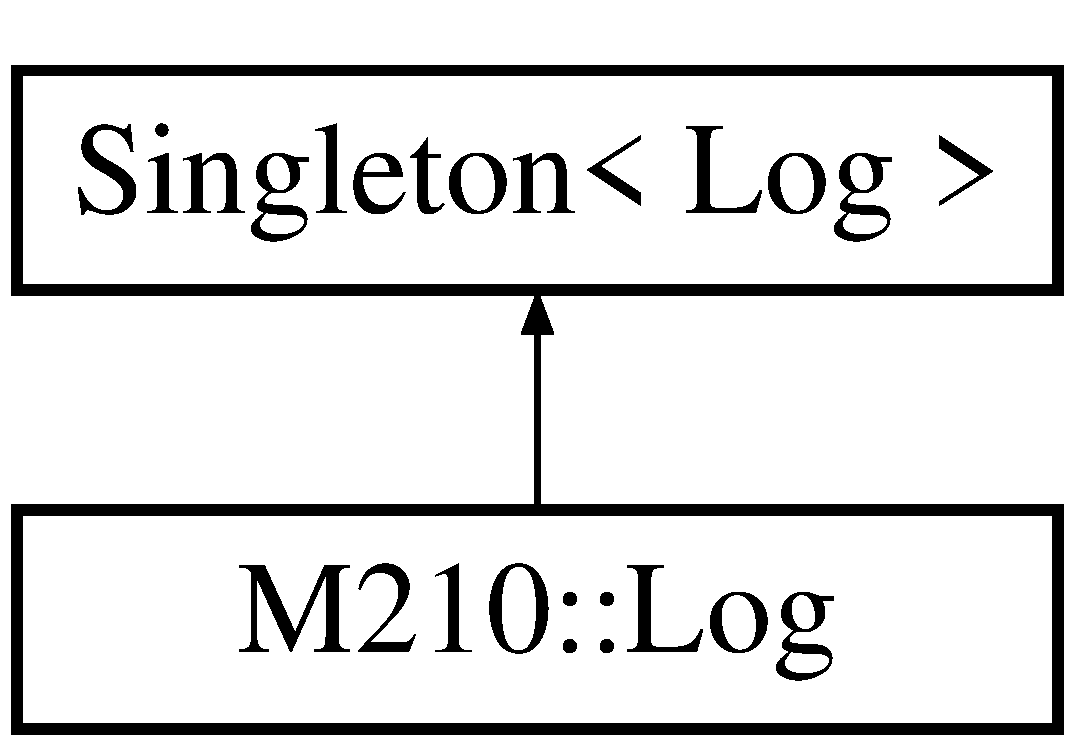
\includegraphics[height=2.000000cm]{class_m210_1_1_log}
\end{center}
\end{figure}
\subsection*{Public Member Functions}
\begin{DoxyCompactItemize}
\item 
\mbox{\Hypertarget{class_m210_1_1_log_a443fed7516e6cf2928a70e42587aa28a}\label{class_m210_1_1_log_a443fed7516e6cf2928a70e42587aa28a}} 
void {\bfseries set\+Flight\+Controller} (\mbox{\hyperlink{class_m210_1_1_flight_controller}{Flight\+Controller}} $\ast$flight\+Controller)
\item 
void \mbox{\hyperlink{class_m210_1_1_log_a83662b0f91b3504917713d0b489b2e7d}{send}} (const char $\ast$type, const char $\ast$format,...)
\end{DoxyCompactItemize}


\subsection{Member Function Documentation}
\mbox{\Hypertarget{class_m210_1_1_log_a83662b0f91b3504917713d0b489b2e7d}\label{class_m210_1_1_log_a83662b0f91b3504917713d0b489b2e7d}} 
\index{M210\+::\+Log@{M210\+::\+Log}!send@{send}}
\index{send@{send}!M210\+::\+Log@{M210\+::\+Log}}
\subsubsection{\texorpdfstring{send()}{send()}}
{\footnotesize\ttfamily void M210\+::\+Log\+::send (\begin{DoxyParamCaption}\item[{const char $\ast$}]{type,  }\item[{const char $\ast$}]{format,  }\item[{}]{... }\end{DoxyParamCaption})}

Send log message to mobile. 
\begin{DoxyParams}{Parameters}
{\em type} & \mbox{\hyperlink{class_m210_1_1_log}{Log}} type (D\+S\+T\+A\+T\+US, D\+E\+R\+R\+OR or D\+D\+E\+B\+UG) \\
\hline
{\em format} & Text to be sent to mobile. Can optionally contain embedded format specifiers that are replaced by the values specified in subsequent additional arguments and formatted as requested. \\
\hline
{\em ...} & Variadic additional arguments \\
\hline
\end{DoxyParams}


The documentation for this class was generated from the following files\+:\begin{DoxyCompactItemize}
\item 
util/\mbox{\hyperlink{_log_8h}{Log.\+h}}\item 
util/\mbox{\hyperlink{_log_8cpp}{Log.\+cpp}}\end{DoxyCompactItemize}

\hypertarget{class_m210_1_1_mobile}{}\section{M210\+:\+:Mobile Class Reference}
\label{class_m210_1_1_mobile}\index{M210\+::\+Mobile@{M210\+::\+Mobile}}
\subsection*{Public Member Functions}
\begin{DoxyCompactItemize}
\item 
\mbox{\hyperlink{class_m210_1_1_mobile_aa3e3dfa96e148844b0f2cfa912e0e615}{Mobile}} (\mbox{\hyperlink{class_m210_1_1_flight_controller}{Flight\+Controller}} $\ast$flight\+Controller)
\item 
void \mbox{\hyperlink{class_m210_1_1_mobile_a9315a171e151194c073ef6101a5a395f}{setup}} ()
\item 
\mbox{\hyperlink{class_m210_1_1_flight_controller}{Flight\+Controller}} $\ast$ \mbox{\hyperlink{class_m210_1_1_mobile_ad4cdcfe5206d1aae2b62c457591ef480}{get\+Flight\+Controller}} () const
\end{DoxyCompactItemize}
\subsection*{Static Public Member Functions}
\begin{DoxyCompactItemize}
\item 
static void \mbox{\hyperlink{class_m210_1_1_mobile_a1213532d9326b0bbb8b679299c93a1a2}{mobile\+Callback}} (Vehicle $\ast$vehicle, Recv\+Container recv\+Frame, User\+Data user\+Data)
\end{DoxyCompactItemize}


\subsection{Constructor \& Destructor Documentation}
\mbox{\Hypertarget{class_m210_1_1_mobile_aa3e3dfa96e148844b0f2cfa912e0e615}\label{class_m210_1_1_mobile_aa3e3dfa96e148844b0f2cfa912e0e615}} 
\index{M210\+::\+Mobile@{M210\+::\+Mobile}!Mobile@{Mobile}}
\index{Mobile@{Mobile}!M210\+::\+Mobile@{M210\+::\+Mobile}}
\subsubsection{\texorpdfstring{Mobile()}{Mobile()}}
{\footnotesize\ttfamily Mobile\+::\+Mobile (\begin{DoxyParamCaption}\item[{\mbox{\hyperlink{class_m210_1_1_flight_controller}{Flight\+Controller}} $\ast$}]{flight\+Controller }\end{DoxyParamCaption})\hspace{0.3cm}{\ttfamily [explicit]}}

Create \mbox{\hyperlink{class_m210_1_1_mobile}{Mobile}} Object 
\begin{DoxyParams}{Parameters}
{\em flight\+Controller} & flight controller to use \\
\hline
\end{DoxyParams}


\subsection{Member Function Documentation}
\mbox{\Hypertarget{class_m210_1_1_mobile_ad4cdcfe5206d1aae2b62c457591ef480}\label{class_m210_1_1_mobile_ad4cdcfe5206d1aae2b62c457591ef480}} 
\index{M210\+::\+Mobile@{M210\+::\+Mobile}!get\+Flight\+Controller@{get\+Flight\+Controller}}
\index{get\+Flight\+Controller@{get\+Flight\+Controller}!M210\+::\+Mobile@{M210\+::\+Mobile}}
\subsubsection{\texorpdfstring{get\+Flight\+Controller()}{getFlightController()}}
{\footnotesize\ttfamily \mbox{\hyperlink{class_m210_1_1_flight_controller}{Flight\+Controller}}$\ast$ M210\+::\+Mobile\+::get\+Flight\+Controller (\begin{DoxyParamCaption}{ }\end{DoxyParamCaption}) const\hspace{0.3cm}{\ttfamily [inline]}}

Get used flight controller \begin{DoxyReturn}{Returns}
Flight controller pointer 
\end{DoxyReturn}
\mbox{\Hypertarget{class_m210_1_1_mobile_a1213532d9326b0bbb8b679299c93a1a2}\label{class_m210_1_1_mobile_a1213532d9326b0bbb8b679299c93a1a2}} 
\index{M210\+::\+Mobile@{M210\+::\+Mobile}!mobile\+Callback@{mobile\+Callback}}
\index{mobile\+Callback@{mobile\+Callback}!M210\+::\+Mobile@{M210\+::\+Mobile}}
\subsubsection{\texorpdfstring{mobile\+Callback()}{mobileCallback()}}
{\footnotesize\ttfamily void Mobile\+::mobile\+Callback (\begin{DoxyParamCaption}\item[{Vehicle $\ast$}]{vehicle,  }\item[{Recv\+Container}]{recv\+Frame,  }\item[{User\+Data}]{user\+Data }\end{DoxyParamCaption})\hspace{0.3cm}{\ttfamily [static]}}

Callback for incoming mobile data. Process data and decide what to do with them 
\begin{DoxyParams}{Parameters}
{\em vehicle} & Vehicle receiving data \\
\hline
{\em recv\+Frame} & Incoming data \\
\hline
{\em user\+Data} & \mbox{\hyperlink{class_m210_1_1_mobile}{Mobile}} object casted as void$\ast$ \\
\hline
\end{DoxyParams}
\mbox{\Hypertarget{class_m210_1_1_mobile_a9315a171e151194c073ef6101a5a395f}\label{class_m210_1_1_mobile_a9315a171e151194c073ef6101a5a395f}} 
\index{M210\+::\+Mobile@{M210\+::\+Mobile}!setup@{setup}}
\index{setup@{setup}!M210\+::\+Mobile@{M210\+::\+Mobile}}
\subsubsection{\texorpdfstring{setup()}{setup()}}
{\footnotesize\ttfamily void Mobile\+::setup (\begin{DoxyParamCaption}{ }\end{DoxyParamCaption})}

Define callback for parsing incoming data 

The documentation for this class was generated from the following files\+:\begin{DoxyCompactItemize}
\item 
Communication/\mbox{\hyperlink{_mobile_8h}{Mobile.\+h}}\item 
Communication/\mbox{\hyperlink{_mobile_8cpp}{Mobile.\+cpp}}\end{DoxyCompactItemize}

\hypertarget{class_m210_1_1_monitored_mission}{}\section{M210\+:\+:Monitored\+Mission Class Reference}
\label{class_m210_1_1_monitored_mission}\index{M210\+::\+Monitored\+Mission@{M210\+::\+Monitored\+Mission}}
\subsection*{Public Member Functions}
\begin{DoxyCompactItemize}
\item 
\mbox{\Hypertarget{class_m210_1_1_monitored_mission_a7f47ae2a0d72c6f28b33c81950b6c215}\label{class_m210_1_1_monitored_mission_a7f47ae2a0d72c6f28b33c81950b6c215}} 
{\bfseries Monitored\+Mission} (\mbox{\hyperlink{class_m210_1_1_flight_controller}{Flight\+Controller}} $\ast$flight\+Controller)
\item 
bool \mbox{\hyperlink{class_m210_1_1_monitored_mission_a70392abfa221992cf46ffddae110ee5a}{take\+Off}} (int timeout=1) const
\item 
bool \mbox{\hyperlink{class_m210_1_1_monitored_mission_aa9c133ca528a6942514a5be8395b4984}{landing}} (int timeout=1) const
\end{DoxyCompactItemize}


\subsection{Member Function Documentation}
\mbox{\Hypertarget{class_m210_1_1_monitored_mission_aa9c133ca528a6942514a5be8395b4984}\label{class_m210_1_1_monitored_mission_aa9c133ca528a6942514a5be8395b4984}} 
\index{M210\+::\+Monitored\+Mission@{M210\+::\+Monitored\+Mission}!landing@{landing}}
\index{landing@{landing}!M210\+::\+Monitored\+Mission@{M210\+::\+Monitored\+Mission}}
\subsubsection{\texorpdfstring{landing()}{landing()}}
{\footnotesize\ttfamily bool Monitored\+Mission\+::landing (\begin{DoxyParamCaption}\item[{int}]{timeout = {\ttfamily 1} }\end{DoxyParamCaption}) const}

Monitored landing. Blocking call 
\begin{DoxyParams}{Parameters}
{\em timeout} & Timeout used on S\+DK method calls \mbox{[}s\mbox{]} \\
\hline
\end{DoxyParams}
\begin{DoxyReturn}{Returns}
true if success
\end{DoxyReturn}
Monitored landing. Return true if success \mbox{\Hypertarget{class_m210_1_1_monitored_mission_a70392abfa221992cf46ffddae110ee5a}\label{class_m210_1_1_monitored_mission_a70392abfa221992cf46ffddae110ee5a}} 
\index{M210\+::\+Monitored\+Mission@{M210\+::\+Monitored\+Mission}!take\+Off@{take\+Off}}
\index{take\+Off@{take\+Off}!M210\+::\+Monitored\+Mission@{M210\+::\+Monitored\+Mission}}
\subsubsection{\texorpdfstring{take\+Off()}{takeOff()}}
{\footnotesize\ttfamily bool Monitored\+Mission\+::take\+Off (\begin{DoxyParamCaption}\item[{int}]{timeout = {\ttfamily 1} }\end{DoxyParamCaption}) const}

Monitored take-\/off. Blocking call 
\begin{DoxyParams}{Parameters}
{\em timeout} & Timeout used on S\+DK method calls \mbox{[}s\mbox{]} \\
\hline
\end{DoxyParams}
\begin{DoxyReturn}{Returns}
true if success 
\end{DoxyReturn}


The documentation for this class was generated from the following files\+:\begin{DoxyCompactItemize}
\item 
Missions/\mbox{\hyperlink{_monitored_mission_8h}{Monitored\+Mission.\+h}}\item 
Missions/\mbox{\hyperlink{_monitored_mission_8cpp}{Monitored\+Mission.\+cpp}}\end{DoxyCompactItemize}

\hypertarget{class_m210_1_1_package_manager}{}\section{M210\+:\+:Package\+Manager Class Reference}
\label{class_m210_1_1_package_manager}\index{M210\+::\+Package\+Manager@{M210\+::\+Package\+Manager}}
Inheritance diagram for M210\+:\+:Package\+Manager\+:\begin{figure}[H]
\begin{center}
\leavevmode
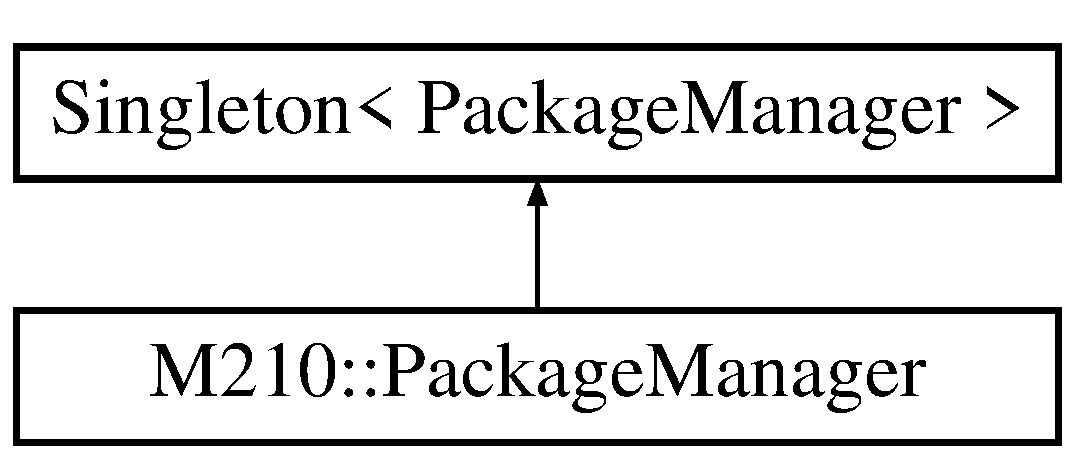
\includegraphics[height=2.000000cm]{class_m210_1_1_package_manager}
\end{center}
\end{figure}
\subsection*{Public Types}
\begin{DoxyCompactItemize}
\item 
enum \mbox{\hyperlink{class_m210_1_1_package_manager_a2da6ff8ace580a0081e1412dd874e21d}{R\+E\+T\+U\+R\+N\+\_\+\+E\+R\+R\+O\+R\+\_\+\+C\+O\+DE}} \{ \newline
\mbox{\hyperlink{class_m210_1_1_package_manager_a2da6ff8ace580a0081e1412dd874e21da7ad0fc69b0a18553d576b9a01118921f}{V\+E\+H\+I\+C\+L\+E\+\_\+\+N\+O\+T\+\_\+\+I\+N\+S\+T\+A\+N\+C\+ED}} = -\/7, 
{\bfseries V\+E\+R\+I\+F\+Y\+\_\+\+F\+A\+I\+L\+ED}, 
{\bfseries I\+N\+V\+A\+L\+I\+D\+\_\+\+I\+N\+D\+EX}, 
{\bfseries S\+T\+A\+R\+T\+\_\+\+P\+A\+C\+K\+A\+G\+E\+\_\+\+F\+A\+I\+L\+ED}, 
\newline
{\bfseries I\+N\+I\+T\+\_\+\+P\+A\+C\+K\+A\+G\+E\+\_\+\+F\+A\+I\+L\+ED}, 
{\bfseries U\+N\+S\+U\+B\+S\+C\+R\+I\+P\+T\+I\+O\+N\+\_\+\+F\+A\+I\+L\+ED}, 
{\bfseries P\+A\+C\+K\+A\+G\+E\+\_\+\+U\+N\+A\+V\+A\+I\+L\+A\+B\+LE}
 \}
\end{DoxyCompactItemize}
\subsection*{Public Member Functions}
\begin{DoxyCompactItemize}
\item 
\mbox{\hyperlink{class_m210_1_1_package_manager_a269a5e51438236422dd3de365ea88860}{Package\+Manager}} ()
\item 
void \mbox{\hyperlink{class_m210_1_1_package_manager_a6c89556663cb2b7484f5819557dc2534}{set\+Vehicle}} (const Vehicle $\ast$vehicle)
\item 
int \mbox{\hyperlink{class_m210_1_1_package_manager_a0448702a3c39e0fc75da71fdf72ebd30}{subscribe}} (Topic\+Name $\ast$topics, int num\+Topic, uint16\+\_\+t frequency, bool enable\+Timestamp)
\item 
int \mbox{\hyperlink{class_m210_1_1_package_manager_a44c8f6bce0db6d2166048b53cef09f9f}{unsubscribe}} (int index)
\item 
void \mbox{\hyperlink{class_m210_1_1_package_manager_a01119dd3d0cc989f95bb7ed4bd94b043}{clear}} ()
\end{DoxyCompactItemize}


\subsection{Member Enumeration Documentation}
\mbox{\Hypertarget{class_m210_1_1_package_manager_a2da6ff8ace580a0081e1412dd874e21d}\label{class_m210_1_1_package_manager_a2da6ff8ace580a0081e1412dd874e21d}} 
\index{M210\+::\+Package\+Manager@{M210\+::\+Package\+Manager}!R\+E\+T\+U\+R\+N\+\_\+\+E\+R\+R\+O\+R\+\_\+\+C\+O\+DE@{R\+E\+T\+U\+R\+N\+\_\+\+E\+R\+R\+O\+R\+\_\+\+C\+O\+DE}}
\index{R\+E\+T\+U\+R\+N\+\_\+\+E\+R\+R\+O\+R\+\_\+\+C\+O\+DE@{R\+E\+T\+U\+R\+N\+\_\+\+E\+R\+R\+O\+R\+\_\+\+C\+O\+DE}!M210\+::\+Package\+Manager@{M210\+::\+Package\+Manager}}
\subsubsection{\texorpdfstring{R\+E\+T\+U\+R\+N\+\_\+\+E\+R\+R\+O\+R\+\_\+\+C\+O\+DE}{RETURN\_ERROR\_CODE}}
{\footnotesize\ttfamily enum \mbox{\hyperlink{class_m210_1_1_package_manager_a2da6ff8ace580a0081e1412dd874e21d}{M210\+::\+Package\+Manager\+::\+R\+E\+T\+U\+R\+N\+\_\+\+E\+R\+R\+O\+R\+\_\+\+C\+O\+DE}}}

\begin{DoxyEnumFields}{Enumerator}
\raisebox{\heightof{T}}[0pt][0pt]{\index{V\+E\+H\+I\+C\+L\+E\+\_\+\+N\+O\+T\+\_\+\+I\+N\+S\+T\+A\+N\+C\+ED@{V\+E\+H\+I\+C\+L\+E\+\_\+\+N\+O\+T\+\_\+\+I\+N\+S\+T\+A\+N\+C\+ED}!M210\+::\+Package\+Manager@{M210\+::\+Package\+Manager}}\index{M210\+::\+Package\+Manager@{M210\+::\+Package\+Manager}!V\+E\+H\+I\+C\+L\+E\+\_\+\+N\+O\+T\+\_\+\+I\+N\+S\+T\+A\+N\+C\+ED@{V\+E\+H\+I\+C\+L\+E\+\_\+\+N\+O\+T\+\_\+\+I\+N\+S\+T\+A\+N\+C\+ED}}}\mbox{\Hypertarget{class_m210_1_1_package_manager_a2da6ff8ace580a0081e1412dd874e21da7ad0fc69b0a18553d576b9a01118921f}\label{class_m210_1_1_package_manager_a2da6ff8ace580a0081e1412dd874e21da7ad0fc69b0a18553d576b9a01118921f}} 
V\+E\+H\+I\+C\+L\+E\+\_\+\+N\+O\+T\+\_\+\+I\+N\+S\+T\+A\+N\+C\+ED&Error code values, have to be negative \\
\hline

\end{DoxyEnumFields}


\subsection{Constructor \& Destructor Documentation}
\mbox{\Hypertarget{class_m210_1_1_package_manager_a269a5e51438236422dd3de365ea88860}\label{class_m210_1_1_package_manager_a269a5e51438236422dd3de365ea88860}} 
\index{M210\+::\+Package\+Manager@{M210\+::\+Package\+Manager}!Package\+Manager@{Package\+Manager}}
\index{Package\+Manager@{Package\+Manager}!M210\+::\+Package\+Manager@{M210\+::\+Package\+Manager}}
\subsubsection{\texorpdfstring{Package\+Manager()}{PackageManager()}}
{\footnotesize\ttfamily Package\+Manager\+::\+Package\+Manager (\begin{DoxyParamCaption}{ }\end{DoxyParamCaption})}

\mbox{\hyperlink{class_m210_1_1_package_manager}{Package\+Manager}} is a singleton 

\subsection{Member Function Documentation}
\mbox{\Hypertarget{class_m210_1_1_package_manager_a01119dd3d0cc989f95bb7ed4bd94b043}\label{class_m210_1_1_package_manager_a01119dd3d0cc989f95bb7ed4bd94b043}} 
\index{M210\+::\+Package\+Manager@{M210\+::\+Package\+Manager}!clear@{clear}}
\index{clear@{clear}!M210\+::\+Package\+Manager@{M210\+::\+Package\+Manager}}
\subsubsection{\texorpdfstring{clear()}{clear()}}
{\footnotesize\ttfamily void Package\+Manager\+::clear (\begin{DoxyParamCaption}{ }\end{DoxyParamCaption})}

Unsubscribe to all subscribed packages \mbox{\Hypertarget{class_m210_1_1_package_manager_a6c89556663cb2b7484f5819557dc2534}\label{class_m210_1_1_package_manager_a6c89556663cb2b7484f5819557dc2534}} 
\index{M210\+::\+Package\+Manager@{M210\+::\+Package\+Manager}!set\+Vehicle@{set\+Vehicle}}
\index{set\+Vehicle@{set\+Vehicle}!M210\+::\+Package\+Manager@{M210\+::\+Package\+Manager}}
\subsubsection{\texorpdfstring{set\+Vehicle()}{setVehicle()}}
{\footnotesize\ttfamily void Package\+Manager\+::set\+Vehicle (\begin{DoxyParamCaption}\item[{const Vehicle $\ast$}]{vehicle }\end{DoxyParamCaption})}

Has to be called before usage to define vehicle to send package 
\begin{DoxyParams}{Parameters}
{\em vehicle} & Pointer to used vehicle \\
\hline
\end{DoxyParams}
\mbox{\Hypertarget{class_m210_1_1_package_manager_a0448702a3c39e0fc75da71fdf72ebd30}\label{class_m210_1_1_package_manager_a0448702a3c39e0fc75da71fdf72ebd30}} 
\index{M210\+::\+Package\+Manager@{M210\+::\+Package\+Manager}!subscribe@{subscribe}}
\index{subscribe@{subscribe}!M210\+::\+Package\+Manager@{M210\+::\+Package\+Manager}}
\subsubsection{\texorpdfstring{subscribe()}{subscribe()}}
{\footnotesize\ttfamily int Package\+Manager\+::subscribe (\begin{DoxyParamCaption}\item[{Topic\+Name $\ast$}]{topics,  }\item[{int}]{num\+Topic,  }\item[{uint16\+\_\+t}]{frequency,  }\item[{bool}]{enable\+Timestamp }\end{DoxyParamCaption})}

Try to allocate package. Setup members of package and start it 
\begin{DoxyParams}{Parameters}
{\em topics} & List of Topic Names to subscribe in the package \\
\hline
{\em num\+Topic} & Number of topics in topics list \\
\hline
{\em frequency} & Package frequency \\
\hline
{\em enable\+Timestamp} & Enable send of transmission package time \\
\hline
\end{DoxyParams}
\begin{DoxyReturn}{Returns}
Negative value of \mbox{\hyperlink{class_m210_1_1_package_manager_a2da6ff8ace580a0081e1412dd874e21d}{Package\+Manager\+::\+R\+E\+T\+U\+R\+N\+\_\+\+E\+R\+R\+O\+R\+\_\+\+C\+O\+DE}} if subscription failed Positive package index if success 
\end{DoxyReturn}
\mbox{\Hypertarget{class_m210_1_1_package_manager_a44c8f6bce0db6d2166048b53cef09f9f}\label{class_m210_1_1_package_manager_a44c8f6bce0db6d2166048b53cef09f9f}} 
\index{M210\+::\+Package\+Manager@{M210\+::\+Package\+Manager}!unsubscribe@{unsubscribe}}
\index{unsubscribe@{unsubscribe}!M210\+::\+Package\+Manager@{M210\+::\+Package\+Manager}}
\subsubsection{\texorpdfstring{unsubscribe()}{unsubscribe()}}
{\footnotesize\ttfamily int Package\+Manager\+::unsubscribe (\begin{DoxyParamCaption}\item[{int}]{index }\end{DoxyParamCaption})}

Unsubscribe from indexed topic 
\begin{DoxyParams}{Parameters}
{\em index} & Package index \\
\hline
\end{DoxyParams}
\begin{DoxyReturn}{Returns}
Negative value of \mbox{\hyperlink{class_m210_1_1_package_manager_a2da6ff8ace580a0081e1412dd874e21d}{Package\+Manager\+::\+R\+E\+T\+U\+R\+N\+\_\+\+E\+R\+R\+O\+R\+\_\+\+C\+O\+DE}} if unsubscription failed 0 if success 
\end{DoxyReturn}


The documentation for this class was generated from the following files\+:\begin{DoxyCompactItemize}
\item 
Managers/\mbox{\hyperlink{_package_manager_8h}{Package\+Manager.\+h}}\item 
Managers/\mbox{\hyperlink{_package_manager_8cpp}{Package\+Manager.\+cpp}}\end{DoxyCompactItemize}

\hypertarget{class_m210_1_1_position_mission}{}\section{M210\+:\+:Position\+Mission Class Reference}
\label{class_m210_1_1_position_mission}\index{M210\+::\+Position\+Mission@{M210\+::\+Position\+Mission}}
\subsection*{Public Member Functions}
\begin{DoxyCompactItemize}
\item 
\mbox{\Hypertarget{class_m210_1_1_position_mission_a3b3a2c4bb91fb6e01b73b0969a79a39a}\label{class_m210_1_1_position_mission_a3b3a2c4bb91fb6e01b73b0969a79a39a}} 
{\bfseries Position\+Mission} (\mbox{\hyperlink{class_m210_1_1_flight_controller}{Flight\+Controller}} $\ast$flight\+Controller)
\item 
void \mbox{\hyperlink{class_m210_1_1_position_mission_a683a572a71e0ace4b63748be39e2d6e8}{move}} (const Vector3f $\ast$position, float yaw)
\item 
void \mbox{\hyperlink{class_m210_1_1_position_mission_ab2f7cf5caff61d1f73df7253bcc097c6}{update}} ()
\end{DoxyCompactItemize}


\subsection{Member Function Documentation}
\mbox{\Hypertarget{class_m210_1_1_position_mission_a683a572a71e0ace4b63748be39e2d6e8}\label{class_m210_1_1_position_mission_a683a572a71e0ace4b63748be39e2d6e8}} 
\index{M210\+::\+Position\+Mission@{M210\+::\+Position\+Mission}!move@{move}}
\index{move@{move}!M210\+::\+Position\+Mission@{M210\+::\+Position\+Mission}}
\subsubsection{\texorpdfstring{move()}{move()}}
{\footnotesize\ttfamily void Position\+Mission\+::move (\begin{DoxyParamCaption}\item[{const Vector3f $\ast$}]{position,  }\item[{float}]{yaw }\end{DoxyParamCaption})}

Allows user to move aircraft in position and yaw mode 
\begin{DoxyParams}{Parameters}
{\em position} & Position relative values to move in X and Y direction \mbox{[}m\mbox{]} x face to north, y face to east Z value is absolute altitude from take-\/off point \\
\hline
{\em yaw} & Absolute yaw angle to set \mbox{[}deg\mbox{]} \\
\hline
\end{DoxyParams}
\mbox{\Hypertarget{class_m210_1_1_position_mission_ab2f7cf5caff61d1f73df7253bcc097c6}\label{class_m210_1_1_position_mission_ab2f7cf5caff61d1f73df7253bcc097c6}} 
\index{M210\+::\+Position\+Mission@{M210\+::\+Position\+Mission}!update@{update}}
\index{update@{update}!M210\+::\+Position\+Mission@{M210\+::\+Position\+Mission}}
\subsubsection{\texorpdfstring{update()}{update()}}
{\footnotesize\ttfamily void Position\+Mission\+::update (\begin{DoxyParamCaption}{ }\end{DoxyParamCaption})}

Has to be called continuously 

The documentation for this class was generated from the following files\+:\begin{DoxyCompactItemize}
\item 
Missions/\mbox{\hyperlink{_position_mission_8h}{Position\+Mission.\+h}}\item 
Missions/\mbox{\hyperlink{_position_mission_8cpp}{Position\+Mission.\+cpp}}\end{DoxyCompactItemize}

\hypertarget{class_m210_1_1_position_offset_mission}{}\section{M210\+:\+:Position\+Offset\+Mission Class Reference}
\label{class_m210_1_1_position_offset_mission}\index{M210\+::\+Position\+Offset\+Mission@{M210\+::\+Position\+Offset\+Mission}}
\subsection*{Public Member Functions}
\begin{DoxyCompactItemize}
\item 
\mbox{\Hypertarget{class_m210_1_1_position_offset_mission_aca7a22775c3d9bd04f780b4754595304}\label{class_m210_1_1_position_offset_mission_aca7a22775c3d9bd04f780b4754595304}} 
{\bfseries Position\+Offset\+Mission} (\mbox{\hyperlink{class_m210_1_1_flight_controller}{Flight\+Controller}} $\ast$flight\+Controller)
\item 
bool \mbox{\hyperlink{class_m210_1_1_position_offset_mission_a0927b9499ed266163a029679ff1723cb}{move}} (const Vector3f $\ast$offset, float yaw, float pos\+Threshold, float yaw\+Threshold)
\item 
bool \mbox{\hyperlink{class_m210_1_1_position_offset_mission_a73b8383335905c16a9a3b9298bbe2d75}{update}} ()
\end{DoxyCompactItemize}


\subsection{Member Function Documentation}
\mbox{\Hypertarget{class_m210_1_1_position_offset_mission_a0927b9499ed266163a029679ff1723cb}\label{class_m210_1_1_position_offset_mission_a0927b9499ed266163a029679ff1723cb}} 
\index{M210\+::\+Position\+Offset\+Mission@{M210\+::\+Position\+Offset\+Mission}!move@{move}}
\index{move@{move}!M210\+::\+Position\+Offset\+Mission@{M210\+::\+Position\+Offset\+Mission}}
\subsubsection{\texorpdfstring{move()}{move()}}
{\footnotesize\ttfamily bool Position\+Offset\+Mission\+::move (\begin{DoxyParamCaption}\item[{const Vector3f $\ast$}]{offset,  }\item[{float}]{yaw,  }\item[{float}]{pos\+Threshold,  }\item[{float}]{yaw\+Threshold }\end{DoxyParamCaption})}

Allows user to move aircraft of an offset from current location. The aircraft will move to that position and stay there. 
\begin{DoxyParams}{Parameters}
{\em offset} & Relative offset vector to move \mbox{[}m\mbox{]} Vector is relative to the ground x face to north, y face to east, z face to sky \\
\hline
{\em yaw} & Absolute yaw angle to set \mbox{[}deg\mbox{]} \\
\hline
{\em pos\+Threshold} & Position threshold used by mission to consider position as reached \mbox{[}m\mbox{]} \\
\hline
{\em yaw\+Threshold} & Angle threshold used by mission to consider angle as reached \mbox{[}deg\mbox{]} \\
\hline
\end{DoxyParams}
\begin{DoxyReturn}{Returns}
true if mission is correctly initialized 
\end{DoxyReturn}
\mbox{\Hypertarget{class_m210_1_1_position_offset_mission_a73b8383335905c16a9a3b9298bbe2d75}\label{class_m210_1_1_position_offset_mission_a73b8383335905c16a9a3b9298bbe2d75}} 
\index{M210\+::\+Position\+Offset\+Mission@{M210\+::\+Position\+Offset\+Mission}!update@{update}}
\index{update@{update}!M210\+::\+Position\+Offset\+Mission@{M210\+::\+Position\+Offset\+Mission}}
\subsubsection{\texorpdfstring{update()}{update()}}
{\footnotesize\ttfamily bool Position\+Offset\+Mission\+::update (\begin{DoxyParamCaption}{ }\end{DoxyParamCaption})}

Has to be called continuously \begin{DoxyReturn}{Returns}
true if destination is reached, false otherwise 
\end{DoxyReturn}


The documentation for this class was generated from the following files\+:\begin{DoxyCompactItemize}
\item 
Missions/\mbox{\hyperlink{_position_offset_mission_8h}{Position\+Offset\+Mission.\+h}}\item 
Missions/\mbox{\hyperlink{_position_offset_mission_8cpp}{Position\+Offset\+Mission.\+cpp}}\end{DoxyCompactItemize}

\hypertarget{class_m210_1_1_thread_manager}{}\section{M210\+:\+:Thread\+Manager Class Reference}
\label{class_m210_1_1_thread_manager}\index{M210\+::\+Thread\+Manager@{M210\+::\+Thread\+Manager}}
\subsection*{Static Public Member Functions}
\begin{DoxyCompactItemize}
\item 
static bool \mbox{\hyperlink{class_m210_1_1_thread_manager_a7a8151ede3e7950e8e092f672f8a790d}{start}} (string name, pthread\+\_\+t $\ast$tid, pthread\+\_\+attr\+\_\+t $\ast$attr, void $\ast$($\ast$thread)(void $\ast$), void $\ast$arg)
\item 
static void \mbox{\hyperlink{class_m210_1_1_thread_manager_a10956e3566cbf7050f16b20bf0cf3280}{stop}} (const pthread\+\_\+t $\ast$id)
\end{DoxyCompactItemize}


\subsection{Member Function Documentation}
\mbox{\Hypertarget{class_m210_1_1_thread_manager_a7a8151ede3e7950e8e092f672f8a790d}\label{class_m210_1_1_thread_manager_a7a8151ede3e7950e8e092f672f8a790d}} 
\index{M210\+::\+Thread\+Manager@{M210\+::\+Thread\+Manager}!start@{start}}
\index{start@{start}!M210\+::\+Thread\+Manager@{M210\+::\+Thread\+Manager}}
\subsubsection{\texorpdfstring{start()}{start()}}
{\footnotesize\ttfamily bool Thread\+Manager\+::start (\begin{DoxyParamCaption}\item[{string}]{name,  }\item[{pthread\+\_\+t $\ast$}]{tid,  }\item[{pthread\+\_\+attr\+\_\+t $\ast$}]{attr,  }\item[{void $\ast$($\ast$)(void $\ast$)}]{thread,  }\item[{void $\ast$}]{arg }\end{DoxyParamCaption})\hspace{0.3cm}{\ttfamily [static]}}

Create and launch thread 
\begin{DoxyParams}{Parameters}
{\em name} & Thread name, restricted to 16 characters \\
\hline
{\em tid} & Points to a pthread\+\_\+t structure in which thread id must be returned \\
\hline
{\em attr} & Points to a pthread\+\_\+attr\+\_\+t structure whose contents are used at thread creation time to determine attributes for the new thread \\
\hline
{\em thread} & Thread routine declared as follow \+: void $\ast$my\+Thread(void $\ast$param) \\
\hline
{\em arg} & Will be passed as argument to thread routine \\
\hline
\end{DoxyParams}
\begin{DoxyReturn}{Returns}
True if thread creation and launch works, false otherwise 
\end{DoxyReturn}
\mbox{\Hypertarget{class_m210_1_1_thread_manager_a10956e3566cbf7050f16b20bf0cf3280}\label{class_m210_1_1_thread_manager_a10956e3566cbf7050f16b20bf0cf3280}} 
\index{M210\+::\+Thread\+Manager@{M210\+::\+Thread\+Manager}!stop@{stop}}
\index{stop@{stop}!M210\+::\+Thread\+Manager@{M210\+::\+Thread\+Manager}}
\subsubsection{\texorpdfstring{stop()}{stop()}}
{\footnotesize\ttfamily void Thread\+Manager\+::stop (\begin{DoxyParamCaption}\item[{const pthread\+\_\+t $\ast$}]{id }\end{DoxyParamCaption})\hspace{0.3cm}{\ttfamily [static]}}

Stop thread Doesn\textquotesingle{}t work -\/ Unused 
\begin{DoxyParams}{Parameters}
{\em id} & Thread id to stop \\
\hline
\end{DoxyParams}


The documentation for this class was generated from the following files\+:\begin{DoxyCompactItemize}
\item 
Managers/\mbox{\hyperlink{_thread_manager_8h}{Thread\+Manager.\+h}}\item 
Managers/\mbox{\hyperlink{_thread_manager_8cpp}{Thread\+Manager.\+cpp}}\end{DoxyCompactItemize}

\hypertarget{class_m210_1_1_uart}{}\section{M210\+:\+:Uart Class Reference}
\label{class_m210_1_1_uart}\index{M210\+::\+Uart@{M210\+::\+Uart}}
\subsection*{Public Member Functions}
\begin{DoxyCompactItemize}
\item 
\mbox{\hyperlink{class_m210_1_1_uart_af1f7108bb9b2519bb0bd6e57990aec07}{Uart}} (const char $\ast$device, uint32\+\_\+t baud\+Rate)
\item 
\mbox{\hyperlink{class_m210_1_1_uart_a7160154094413395a23dbaa287dbef3c}{$\sim$\+Uart}} ()
\item 
void \mbox{\hyperlink{class_m210_1_1_uart_a7aa2fba14c420024a1e2ec9079684def}{send}} (const uint8\+\_\+t $\ast$buf, size\+\_\+t len) const
\item 
bool \mbox{\hyperlink{class_m210_1_1_uart_ad793a587c421c2e8d6bde5d6ddfd95d8}{launch\+Rx\+Thread}} ()
\item 
void \mbox{\hyperlink{class_m210_1_1_uart_a294e7c110b8bb09dd7b4fde43ed1fce4}{set\+Flight\+Controller}} (const \mbox{\hyperlink{class_m210_1_1_flight_controller}{Flight\+Controller}} $\ast$flight\+Controller)
\end{DoxyCompactItemize}


\subsection{Constructor \& Destructor Documentation}
\mbox{\Hypertarget{class_m210_1_1_uart_af1f7108bb9b2519bb0bd6e57990aec07}\label{class_m210_1_1_uart_af1f7108bb9b2519bb0bd6e57990aec07}} 
\index{M210\+::\+Uart@{M210\+::\+Uart}!Uart@{Uart}}
\index{Uart@{Uart}!M210\+::\+Uart@{M210\+::\+Uart}}
\subsubsection{\texorpdfstring{Uart()}{Uart()}}
{\footnotesize\ttfamily Uart\+::\+Uart (\begin{DoxyParamCaption}\item[{const char $\ast$}]{device,  }\item[{uint32\+\_\+t}]{baud\+Rate }\end{DoxyParamCaption})}

Create serial device with D\+JI Linux\+Serial\+Device class and initialize it 
\begin{DoxyParams}{Parameters}
{\em device} & Linux serial device port \\
\hline
{\em baud\+Rate} & Baud rate \mbox{[}Bd\mbox{]} \\
\hline
\end{DoxyParams}
\mbox{\Hypertarget{class_m210_1_1_uart_a7160154094413395a23dbaa287dbef3c}\label{class_m210_1_1_uart_a7160154094413395a23dbaa287dbef3c}} 
\index{M210\+::\+Uart@{M210\+::\+Uart}!````~Uart@{$\sim$\+Uart}}
\index{````~Uart@{$\sim$\+Uart}!M210\+::\+Uart@{M210\+::\+Uart}}
\subsubsection{\texorpdfstring{$\sim$\+Uart()}{~Uart()}}
{\footnotesize\ttfamily Uart\+::$\sim$\+Uart (\begin{DoxyParamCaption}{ }\end{DoxyParamCaption})}

Delete serial device 

\subsection{Member Function Documentation}
\mbox{\Hypertarget{class_m210_1_1_uart_ad793a587c421c2e8d6bde5d6ddfd95d8}\label{class_m210_1_1_uart_ad793a587c421c2e8d6bde5d6ddfd95d8}} 
\index{M210\+::\+Uart@{M210\+::\+Uart}!launch\+Rx\+Thread@{launch\+Rx\+Thread}}
\index{launch\+Rx\+Thread@{launch\+Rx\+Thread}!M210\+::\+Uart@{M210\+::\+Uart}}
\subsubsection{\texorpdfstring{launch\+Rx\+Thread()}{launchRxThread()}}
{\footnotesize\ttfamily bool Uart\+::launch\+Rx\+Thread (\begin{DoxyParamCaption}{ }\end{DoxyParamCaption})}

Launch uart rx thread \begin{DoxyReturn}{Returns}
true if thread creation and launch works, false otherwise 
\end{DoxyReturn}
\mbox{\Hypertarget{class_m210_1_1_uart_a7aa2fba14c420024a1e2ec9079684def}\label{class_m210_1_1_uart_a7aa2fba14c420024a1e2ec9079684def}} 
\index{M210\+::\+Uart@{M210\+::\+Uart}!send@{send}}
\index{send@{send}!M210\+::\+Uart@{M210\+::\+Uart}}
\subsubsection{\texorpdfstring{send()}{send()}}
{\footnotesize\ttfamily void Uart\+::send (\begin{DoxyParamCaption}\item[{const uint8\+\_\+t $\ast$}]{buf,  }\item[{size\+\_\+t}]{len }\end{DoxyParamCaption}) const}

Send data by uart 
\begin{DoxyParams}{Parameters}
{\em buf} & Buffer pointer \\
\hline
{\em len} & data length \\
\hline
\end{DoxyParams}
\mbox{\Hypertarget{class_m210_1_1_uart_a294e7c110b8bb09dd7b4fde43ed1fce4}\label{class_m210_1_1_uart_a294e7c110b8bb09dd7b4fde43ed1fce4}} 
\index{M210\+::\+Uart@{M210\+::\+Uart}!set\+Flight\+Controller@{set\+Flight\+Controller}}
\index{set\+Flight\+Controller@{set\+Flight\+Controller}!M210\+::\+Uart@{M210\+::\+Uart}}
\subsubsection{\texorpdfstring{set\+Flight\+Controller()}{setFlightController()}}
{\footnotesize\ttfamily void M210\+::\+Uart\+::set\+Flight\+Controller (\begin{DoxyParamCaption}\item[{const \mbox{\hyperlink{class_m210_1_1_flight_controller}{Flight\+Controller}} $\ast$}]{flight\+Controller }\end{DoxyParamCaption})\hspace{0.3cm}{\ttfamily [inline]}}

Configure flight controller to use 
\begin{DoxyParams}{Parameters}
{\em flight\+Controller} & Flight controller pointer \\
\hline
\end{DoxyParams}


The documentation for this class was generated from the following files\+:\begin{DoxyCompactItemize}
\item 
Communication/\mbox{\hyperlink{_uart_8h}{Uart.\+h}}\item 
Communication/\mbox{\hyperlink{_uart_8cpp}{Uart.\+cpp}}\end{DoxyCompactItemize}

\hypertarget{struct_vector2}{}\section{Vector2 Struct Reference}
\label{struct_vector2}\index{Vector2@{Vector2}}
\subsection*{Public Attributes}
\begin{DoxyCompactItemize}
\item 
\mbox{\Hypertarget{struct_vector2_a61d73d9036ccbb3257fbe595c014a1d0}\label{struct_vector2_a61d73d9036ccbb3257fbe595c014a1d0}} 
double {\bfseries x}
\item 
\mbox{\Hypertarget{struct_vector2_a4df9b2a8e79e6e30a7a3b34722d8b8b8}\label{struct_vector2_a4df9b2a8e79e6e30a7a3b34722d8b8b8}} 
double {\bfseries y}
\end{DoxyCompactItemize}


The documentation for this struct was generated from the following file\+:\begin{DoxyCompactItemize}
\item 
util/\mbox{\hyperlink{define_8h}{define.\+h}}\end{DoxyCompactItemize}

\hypertarget{class_m210_1_1_velocity_mission}{}\section{M210\+:\+:Velocity\+Mission Class Reference}
\label{class_m210_1_1_velocity_mission}\index{M210\+::\+Velocity\+Mission@{M210\+::\+Velocity\+Mission}}
\subsection*{Public Member Functions}
\begin{DoxyCompactItemize}
\item 
\mbox{\Hypertarget{class_m210_1_1_velocity_mission_aebd12135407bb5c9487ec1a5d9ec3966}\label{class_m210_1_1_velocity_mission_aebd12135407bb5c9487ec1a5d9ec3966}} 
{\bfseries Velocity\+Mission} (\mbox{\hyperlink{class_m210_1_1_flight_controller}{Flight\+Controller}} $\ast$flight\+Controller)
\item 
void \mbox{\hyperlink{class_m210_1_1_velocity_mission_a35a436e3ae0c48014334ccd5d2868861}{move}} (const Vector3f $\ast$velocity, float yaw)
\item 
void \mbox{\hyperlink{class_m210_1_1_velocity_mission_a709e74d4c01378c7cd2bcbab602bba2c}{update}} ()
\end{DoxyCompactItemize}


\subsection{Member Function Documentation}
\mbox{\Hypertarget{class_m210_1_1_velocity_mission_a35a436e3ae0c48014334ccd5d2868861}\label{class_m210_1_1_velocity_mission_a35a436e3ae0c48014334ccd5d2868861}} 
\index{M210\+::\+Velocity\+Mission@{M210\+::\+Velocity\+Mission}!move@{move}}
\index{move@{move}!M210\+::\+Velocity\+Mission@{M210\+::\+Velocity\+Mission}}
\subsubsection{\texorpdfstring{move()}{move()}}
{\footnotesize\ttfamily void Velocity\+Mission\+::move (\begin{DoxyParamCaption}\item[{const Vector3f $\ast$}]{velocity,  }\item[{float}]{yaw }\end{DoxyParamCaption})}

Velocity Control. Allows user to set a velocity vector. The aircraft will move as described by vector until \mbox{\hyperlink{class_m210_1_1_velocity_mission_a709e74d4c01378c7cd2bcbab602bba2c}{update()}} is no more called. 
\begin{DoxyParams}{Parameters}
{\em velocity} & Absolute velocity vector to set \mbox{[}m/s\mbox{]} Vector is relative to the ground x face to north, y face to east, z face to sky \\
\hline
{\em yaw} & Absolute yaw rate to set \mbox{[}deg/s\mbox{]} \\
\hline
\end{DoxyParams}
\mbox{\Hypertarget{class_m210_1_1_velocity_mission_a709e74d4c01378c7cd2bcbab602bba2c}\label{class_m210_1_1_velocity_mission_a709e74d4c01378c7cd2bcbab602bba2c}} 
\index{M210\+::\+Velocity\+Mission@{M210\+::\+Velocity\+Mission}!update@{update}}
\index{update@{update}!M210\+::\+Velocity\+Mission@{M210\+::\+Velocity\+Mission}}
\subsubsection{\texorpdfstring{update()}{update()}}
{\footnotesize\ttfamily void Velocity\+Mission\+::update (\begin{DoxyParamCaption}{ }\end{DoxyParamCaption})}

Has to be called frequently to send moving order to the aircraft. D\+JI recommend to send orders at 50\+Hz 

The documentation for this class was generated from the following files\+:\begin{DoxyCompactItemize}
\item 
Missions/\mbox{\hyperlink{_velocity_mission_8h}{Velocity\+Mission.\+h}}\item 
Missions/\mbox{\hyperlink{_velocity_mission_8cpp}{Velocity\+Mission.\+cpp}}\end{DoxyCompactItemize}

\hypertarget{class_m210_1_1_watchdog}{}\section{M210\+:\+:Watchdog Class Reference}
\label{class_m210_1_1_watchdog}\index{M210\+::\+Watchdog@{M210\+::\+Watchdog}}
\subsection*{Public Member Functions}
\begin{DoxyCompactItemize}
\item 
\mbox{\hyperlink{class_m210_1_1_watchdog_a4a992183689c0800d586f6a6daacc7b4}{Watchdog}} (unsigned limit)
\item 
void \mbox{\hyperlink{class_m210_1_1_watchdog_a4342960b3b6881def5dc2342fee990ba}{increment}} ()
\item 
void \mbox{\hyperlink{class_m210_1_1_watchdog_ad64f941736836164bf9049ead5ca31b2}{reset}} ()
\item 
bool \mbox{\hyperlink{class_m210_1_1_watchdog_a235a91f4745f75bd5222ecc57d01f9ef}{is\+Enabled}} ()
\end{DoxyCompactItemize}


\subsection{Constructor \& Destructor Documentation}
\mbox{\Hypertarget{class_m210_1_1_watchdog_a4a992183689c0800d586f6a6daacc7b4}\label{class_m210_1_1_watchdog_a4a992183689c0800d586f6a6daacc7b4}} 
\index{M210\+::\+Watchdog@{M210\+::\+Watchdog}!Watchdog@{Watchdog}}
\index{Watchdog@{Watchdog}!M210\+::\+Watchdog@{M210\+::\+Watchdog}}
\subsubsection{\texorpdfstring{Watchdog()}{Watchdog()}}
{\footnotesize\ttfamily Watchdog\+::\+Watchdog (\begin{DoxyParamCaption}\item[{unsigned}]{limit }\end{DoxyParamCaption})\hspace{0.3cm}{\ttfamily [explicit]}}

Create watchdog 
\begin{DoxyParams}{Parameters}
{\em limit} & Numbers of orders that can be sent to aircraft before watchdog is triggered Relative watchdog duration depends on order sending frequency. See \mbox{\hyperlink{class_m210_1_1_flight_controller}{Flight\+Controller}} thread \\
\hline
\end{DoxyParams}


\subsection{Member Function Documentation}
\mbox{\Hypertarget{class_m210_1_1_watchdog_a4342960b3b6881def5dc2342fee990ba}\label{class_m210_1_1_watchdog_a4342960b3b6881def5dc2342fee990ba}} 
\index{M210\+::\+Watchdog@{M210\+::\+Watchdog}!increment@{increment}}
\index{increment@{increment}!M210\+::\+Watchdog@{M210\+::\+Watchdog}}
\subsubsection{\texorpdfstring{increment()}{increment()}}
{\footnotesize\ttfamily void Watchdog\+::increment (\begin{DoxyParamCaption}{ }\end{DoxyParamCaption})}

Increment local counter \mbox{\Hypertarget{class_m210_1_1_watchdog_a235a91f4745f75bd5222ecc57d01f9ef}\label{class_m210_1_1_watchdog_a235a91f4745f75bd5222ecc57d01f9ef}} 
\index{M210\+::\+Watchdog@{M210\+::\+Watchdog}!is\+Enabled@{is\+Enabled}}
\index{is\+Enabled@{is\+Enabled}!M210\+::\+Watchdog@{M210\+::\+Watchdog}}
\subsubsection{\texorpdfstring{is\+Enabled()}{isEnabled()}}
{\footnotesize\ttfamily bool Watchdog\+::is\+Enabled (\begin{DoxyParamCaption}{ }\end{DoxyParamCaption})}

Verify watchdog and display error message on first call (until watchdog is reset) \begin{DoxyReturn}{Returns}
True if watchdog is enabled 
\end{DoxyReturn}
\mbox{\Hypertarget{class_m210_1_1_watchdog_ad64f941736836164bf9049ead5ca31b2}\label{class_m210_1_1_watchdog_ad64f941736836164bf9049ead5ca31b2}} 
\index{M210\+::\+Watchdog@{M210\+::\+Watchdog}!reset@{reset}}
\index{reset@{reset}!M210\+::\+Watchdog@{M210\+::\+Watchdog}}
\subsubsection{\texorpdfstring{reset()}{reset()}}
{\footnotesize\ttfamily void Watchdog\+::reset (\begin{DoxyParamCaption}{ }\end{DoxyParamCaption})}

Reset local counter 

The documentation for this class was generated from the following files\+:\begin{DoxyCompactItemize}
\item 
Aircraft/\mbox{\hyperlink{_watchdog_8h}{Watchdog.\+h}}\item 
Aircraft/\mbox{\hyperlink{_watchdog_8cpp}{Watchdog.\+cpp}}\end{DoxyCompactItemize}

\hypertarget{class_m210_1_1_waypoint_mission}{}\section{M210\+:\+:Waypoint\+Mission Class Reference}
\label{class_m210_1_1_waypoint_mission}\index{M210\+::\+Waypoint\+Mission@{M210\+::\+Waypoint\+Mission}}
\subsection*{Public Member Functions}
\begin{DoxyCompactItemize}
\item 
\mbox{\hyperlink{class_m210_1_1_waypoint_mission_adceae05e862690ed217c8b70aca123a2}{Waypoint\+Mission}} (\mbox{\hyperlink{class_m210_1_1_flight_controller}{Flight\+Controller}} $\ast$flight\+Controller)
\item 
void \mbox{\hyperlink{class_m210_1_1_waypoint_mission_ab4f5a1e359026ddcd640cda09501fd6b}{action}} (unsigned int task)
\end{DoxyCompactItemize}


\subsection{Constructor \& Destructor Documentation}
\mbox{\Hypertarget{class_m210_1_1_waypoint_mission_adceae05e862690ed217c8b70aca123a2}\label{class_m210_1_1_waypoint_mission_adceae05e862690ed217c8b70aca123a2}} 
\index{M210\+::\+Waypoint\+Mission@{M210\+::\+Waypoint\+Mission}!Waypoint\+Mission@{Waypoint\+Mission}}
\index{Waypoint\+Mission@{Waypoint\+Mission}!M210\+::\+Waypoint\+Mission@{M210\+::\+Waypoint\+Mission}}
\subsubsection{\texorpdfstring{Waypoint\+Mission()}{WaypointMission()}}
{\footnotesize\ttfamily M210\+::\+Waypoint\+Mission\+::\+Waypoint\+Mission (\begin{DoxyParamCaption}\item[{\mbox{\hyperlink{class_m210_1_1_flight_controller}{Flight\+Controller}} $\ast$}]{flight\+Controller }\end{DoxyParamCaption})\hspace{0.3cm}{\ttfamily [explicit]}}

Waypoints mission constructor 
\begin{DoxyParams}{Parameters}
{\em flight\+Controller} & The flight controller concerned by the mission \\
\hline
\end{DoxyParams}


\subsection{Member Function Documentation}
\mbox{\Hypertarget{class_m210_1_1_waypoint_mission_ab4f5a1e359026ddcd640cda09501fd6b}\label{class_m210_1_1_waypoint_mission_ab4f5a1e359026ddcd640cda09501fd6b}} 
\index{M210\+::\+Waypoint\+Mission@{M210\+::\+Waypoint\+Mission}!action@{action}}
\index{action@{action}!M210\+::\+Waypoint\+Mission@{M210\+::\+Waypoint\+Mission}}
\subsubsection{\texorpdfstring{action()}{action()}}
{\footnotesize\ttfamily void M210\+::\+Waypoint\+Mission\+::action (\begin{DoxyParamCaption}\item[{unsigned int}]{task }\end{DoxyParamCaption})}

Modify action flow with a mission task 
\begin{DoxyParams}{Parameters}
{\em task} & Task to do, value of \mbox{\hyperlink{class_m210_1_1_action_a0bb36f0932c930e1193428e3c3c98046}{Action\+::\+Mission\+Action}} structure \\
\hline
\end{DoxyParams}


The documentation for this class was generated from the following files\+:\begin{DoxyCompactItemize}
\item 
Missions/\mbox{\hyperlink{_waypoints_mission_8h}{Waypoints\+Mission.\+h}}\item 
Missions/\mbox{\hyperlink{_waypoints_mission_8cpp}{Waypoints\+Mission.\+cpp}}\end{DoxyCompactItemize}

\chapter{File Documentation}
\hypertarget{_action_8cpp}{}\section{Action/\+Action.cpp File Reference}
\label{_action_8cpp}\index{Action/\+Action.\+cpp@{Action/\+Action.\+cpp}}


\mbox{\hyperlink{_action_8h}{Action.\+h}} implementation.  


{\ttfamily \#include $<$fcntl.\+h$>$}\newline
{\ttfamily \#include $<$cassert$>$}\newline
{\ttfamily \#include \char`\"{}Action.\+h\char`\"{}}\newline
{\ttfamily \#include \char`\"{}Action\+Data.\+h\char`\"{}}\newline
{\ttfamily \#include \char`\"{}../\+Aircraft/\+Flight\+Controller.\+h\char`\"{}}\newline
{\ttfamily \#include \char`\"{}../\+Aircraft/\+Watchdog.\+h\char`\"{}}\newline
{\ttfamily \#include \char`\"{}../util/\+Log.\+h\char`\"{}}\newline


\subsection{Detailed Description}
\mbox{\hyperlink{_action_8h}{Action.\+h}} implementation. 

\begin{DoxyVersion}{Version}
1.\+0 
\end{DoxyVersion}
\begin{DoxyDate}{Date}
Jul 18 2018 
\end{DoxyDate}
\begin{DoxyAuthor}{Author}
Jonathan Michel 
\end{DoxyAuthor}

\hypertarget{_action_8h}{}\section{Action/\+Action.h File Reference}
\label{_action_8h}\index{Action/\+Action.\+h@{Action/\+Action.\+h}}


This class provides a queue used to add action to do by Flight\+Controller.  


{\ttfamily \#include $<$pthread.\+h$>$}\newline
{\ttfamily \#include $<$mqueue.\+h$>$}\newline
{\ttfamily \#include $<$dji\+\_\+vehicle.\+hpp$>$}\newline
\subsection*{Classes}
\begin{DoxyCompactItemize}
\item 
class \mbox{\hyperlink{class_m210_1_1_action}{M210\+::\+Action}}
\end{DoxyCompactItemize}
\subsection*{Macros}
\begin{DoxyCompactItemize}
\item 
\mbox{\Hypertarget{_action_8h_a69ba0694e789ac10c827babe30e2a9ee}\label{_action_8h_a69ba0694e789ac10c827babe30e2a9ee}} 
\#define {\bfseries A\+C\+T\+I\+O\+N\+\_\+\+Q\+U\+E\+U\+E\+\_\+\+N\+A\+ME}~\char`\"{}/action\+Queue\char`\"{}
\end{DoxyCompactItemize}


\subsection{Detailed Description}
This class provides a queue used to add action to do by Flight\+Controller. 

\begin{DoxyVersion}{Version}
1.\+0 
\end{DoxyVersion}
\begin{DoxyDate}{Date}
Jul 18 2018 
\end{DoxyDate}
\begin{DoxyAuthor}{Author}
Jonathan Michel Queue is filled on data reception from mobile S\+DK or console Queue is continuously processed in main Action are Action\+Data objects, see \mbox{\hyperlink{_action_data_8h}{Action\+Data.\+h}} mqueue.\+h is used 
\end{DoxyAuthor}

\hypertarget{_action_data_8cpp}{}\section{Action/\+Action\+Data.cpp File Reference}
\label{_action_data_8cpp}\index{Action/\+Action\+Data.\+cpp@{Action/\+Action\+Data.\+cpp}}


\mbox{\hyperlink{_action_data_8h}{Action\+Data.\+h}} implementation.  


{\ttfamily \#include \char`\"{}Action\+Data.\+h\char`\"{}}\newline
{\ttfamily \#include $<$cassert$>$}\newline
{\ttfamily \#include $<$cstring$>$}\newline
{\ttfamily \#include $<$cstddef$>$}\newline


\subsection{Detailed Description}
\mbox{\hyperlink{_action_data_8h}{Action\+Data.\+h}} implementation. 

\begin{DoxyVersion}{Version}
1.\+0 
\end{DoxyVersion}
\begin{DoxyDate}{Date}
Jul 20 2018 
\end{DoxyDate}
\begin{DoxyAuthor}{Author}
Jonathan Michel 
\end{DoxyAuthor}

\hypertarget{_action_data_8h}{}\section{Action/\+Action\+Data.h File Reference}
\label{_action_data_8h}\index{Action/\+Action\+Data.\+h@{Action/\+Action\+Data.\+h}}


Action\+Data objects are added in Action queue (\mbox{\hyperlink{_action_8h}{Action.\+h}}) The goal is to provide an object with variable data size.  


{\ttfamily \#include $<$pthread.\+h$>$}\newline
{\ttfamily \#include $<$dji\+\_\+vehicle.\+hpp$>$}\newline
\subsection*{Classes}
\begin{DoxyCompactItemize}
\item 
class \mbox{\hyperlink{class_m210_1_1_action_data}{M210\+::\+Action\+Data}}
\end{DoxyCompactItemize}
\subsection*{Macros}
\begin{DoxyCompactItemize}
\item 
\#define \mbox{\hyperlink{_action_data_8h_ab2c23ab476d4f7a0207895fe1ab00e50}{\+\_\+\+\_\+push}}(\+\_\+data\+\_\+,  \+\_\+length\+\_\+)
\item 
\#define \mbox{\hyperlink{_action_data_8h_af32898bff77f8e81bd43ad0f30d25221}{\+\_\+push}}(\+\_\+data\+\_\+,  \+\_\+type\+\_\+)
\item 
\#define \mbox{\hyperlink{_action_data_8h_a4f0419f16d53bad043d5f85da427969d}{\+\_\+pop}}(\+\_\+data\+\_\+,  \+\_\+type\+\_\+)
\end{DoxyCompactItemize}


\subsection{Detailed Description}
Action\+Data objects are added in Action queue (\mbox{\hyperlink{_action_8h}{Action.\+h}}) The goal is to provide an object with variable data size. 

\begin{DoxyVersion}{Version}
1.\+0 
\end{DoxyVersion}
\begin{DoxyDate}{Date}
Jul 20 2018 
\end{DoxyDate}
\begin{DoxyAuthor}{Author}
Jonathan Michel It is useful because all actions doesn\textquotesingle{}t need the same amount of data. On object creation, dynamic memory is allocated. Size depends of user need. Data can next be pushed (not all type are yet supported, only main ones). Then, data can be recovered with pop method. /!\textbackslash{} Push/\+Pop methods works as a lifo, last pushed value will be first popped Example of use in unit\+Test() method 
\end{DoxyAuthor}


\subsection{Macro Definition Documentation}
\mbox{\Hypertarget{_action_data_8h_ab2c23ab476d4f7a0207895fe1ab00e50}\label{_action_data_8h_ab2c23ab476d4f7a0207895fe1ab00e50}} 
\index{Action\+Data.\+h@{Action\+Data.\+h}!\+\_\+\+\_\+push@{\+\_\+\+\_\+push}}
\index{\+\_\+\+\_\+push@{\+\_\+\+\_\+push}!Action\+Data.\+h@{Action\+Data.\+h}}
\subsubsection{\texorpdfstring{\+\_\+\+\_\+push}{\_\_push}}
{\footnotesize\ttfamily \#define \+\_\+\+\_\+push(\begin{DoxyParamCaption}\item[{}]{\+\_\+data\+\_\+,  }\item[{}]{\+\_\+length\+\_\+ }\end{DoxyParamCaption})}

{\bfseries Value\+:}
\begin{DoxyCode}
\{                                                       \(\backslash\)
    pthread\_mutex\_lock(&mutex);                         \(\backslash\)
    \textcolor{comment}{/* Copy data in dynamic memory allocated if there */}\(\backslash\)
    \textcolor{comment}{/* is enough place                                */}\(\backslash\)
    auto ptr = \textcolor{keyword}{reinterpret\_cast<}\textcolor{keyword}{const }\textcolor{keywordtype}{char} *\textcolor{keyword}{>}(\_data\_);  \(\backslash\)
    if(!checkSize(\_length\_)) \{                          \(\backslash\)
        DERROR(\textcolor{stringliteral}{"Unable to push data"});                  \(\backslash\)
        pthread\_mutex\_unlock(&mutex);                   \(\backslash\)
        return \textcolor{keyword}{false};                                   \(\backslash\)
    \}                                                   \(\backslash\)
    memcpy(dataPtr + dataPosCnt, ptr, \_length\_);        \(\backslash\)
    dataPosCnt += (\_length\_);                             \(\backslash\)
    pthread\_mutex\_unlock(&mutex);                       \(\backslash\)
    return \textcolor{keyword}{true};                                        \(\backslash\)
\}
\end{DoxyCode}
Copy data to allocated dynamic memory 
\begin{DoxyParams}{Parameters}
{\em \+\_\+data\+\_\+} & Pointer to data to copy \\
\hline
{\em \+\_\+length\+\_\+} & Length of data to copy \mbox{[}bytes\mbox{]} \\
\hline
\end{DoxyParams}
\begin{DoxyReturn}{Returns}
False if there is not enough memory allocated, true otherwise 
\end{DoxyReturn}
\mbox{\Hypertarget{_action_data_8h_a4f0419f16d53bad043d5f85da427969d}\label{_action_data_8h_a4f0419f16d53bad043d5f85da427969d}} 
\index{Action\+Data.\+h@{Action\+Data.\+h}!\+\_\+pop@{\+\_\+pop}}
\index{\+\_\+pop@{\+\_\+pop}!Action\+Data.\+h@{Action\+Data.\+h}}
\subsubsection{\texorpdfstring{\+\_\+pop}{\_pop}}
{\footnotesize\ttfamily \#define \+\_\+pop(\begin{DoxyParamCaption}\item[{}]{\+\_\+data\+\_\+,  }\item[{}]{\+\_\+type\+\_\+ }\end{DoxyParamCaption})}

{\bfseries Value\+:}
\begin{DoxyCode}
\{                                                   \(\backslash\)
    pthread\_mutex\_lock(&mutex);                     \(\backslash\)
    \textcolor{comment}{/* Pop data from dynamic memory allocated if */} \(\backslash\)
    \textcolor{comment}{/* there is remaining data                   */} \(\backslash\)
    size\_t length = \textcolor{keyword}{sizeof}(\_type\_);                 \(\backslash\)
    if(dataPosCnt < length) \{                       \(\backslash\)
        DERROR(\textcolor{stringliteral}{"Unable to pop %s"}, #\_type\_);        \(\backslash\)
        pthread\_mutex\_unlock(&mutex);               \(\backslash\)
        return \textcolor{keyword}{false};                               \(\backslash\)
    \}                                               \(\backslash\)
    dataPosCnt -= length;                           \(\backslash\)
    memcpy(&(\_data\_), dataPtr + dataPosCnt, length);  \(\backslash\)
    pthread\_mutex\_unlock(&mutex);                   \(\backslash\)
    return \textcolor{keyword}{true};                                    \(\backslash\)
\}
\end{DoxyCode}
Read data from dynamic memory 
\begin{DoxyParams}{Parameters}
{\em \+\_\+data\+\_\+} & Pointer to data where write result \\
\hline
{\em \+\_\+type\+\_\+} & Type of data to read \\
\hline
\end{DoxyParams}
\begin{DoxyReturn}{Returns}
False if there is no more data to read in allocated dynamic memory, true otherwise 
\end{DoxyReturn}
\mbox{\Hypertarget{_action_data_8h_af32898bff77f8e81bd43ad0f30d25221}\label{_action_data_8h_af32898bff77f8e81bd43ad0f30d25221}} 
\index{Action\+Data.\+h@{Action\+Data.\+h}!\+\_\+push@{\+\_\+push}}
\index{\+\_\+push@{\+\_\+push}!Action\+Data.\+h@{Action\+Data.\+h}}
\subsubsection{\texorpdfstring{\+\_\+push}{\_push}}
{\footnotesize\ttfamily \#define \+\_\+push(\begin{DoxyParamCaption}\item[{}]{\+\_\+data\+\_\+,  }\item[{}]{\+\_\+type\+\_\+ }\end{DoxyParamCaption})}

{\bfseries Value\+:}
\begin{DoxyCode}
\{                                       \(\backslash\)
    \_\_push(\_data\_, \textcolor{keyword}{sizeof}(\_type\_));     \(\backslash\)
\}
\end{DoxyCode}
Copy data to allocated dynamic memory 
\begin{DoxyParams}{Parameters}
{\em \+\_\+data\+\_\+} & Pointer to data to copy \\
\hline
{\em \+\_\+type\+\_\+} & Type of data to copy \\
\hline
\end{DoxyParams}
\begin{DoxyReturn}{Returns}
False if there is not enough memory allocated, true otherwise 
\end{DoxyReturn}

\hypertarget{_emergency_8cpp}{}\section{Aircraft/\+Emergency.cpp File Reference}
\label{_emergency_8cpp}\index{Aircraft/\+Emergency.\+cpp@{Aircraft/\+Emergency.\+cpp}}


\mbox{\hyperlink{_emergency_8h}{Emergency.\+h}} implementation.  


{\ttfamily \#include \char`\"{}Emergency.\+h\char`\"{}}\newline
{\ttfamily \#include \char`\"{}dji\+\_\+vehicle.\+hpp\char`\"{}}\newline
{\ttfamily \#include \char`\"{}../util/\+Log.\+h\char`\"{}}\newline


\subsection{Detailed Description}
\mbox{\hyperlink{_emergency_8h}{Emergency.\+h}} implementation. 

\begin{DoxyVersion}{Version}
1.\+0 
\end{DoxyVersion}
\begin{DoxyDate}{Date}
juil. 25 2018 
\end{DoxyDate}
\begin{DoxyAuthor}{Author}
Jonathan Michel 
\end{DoxyAuthor}

\hypertarget{_emergency_8h}{}\section{Aircraft/\+Emergency.h File Reference}
\label{_emergency_8h}\index{Aircraft/\+Emergency.\+h@{Aircraft/\+Emergency.\+h}}


This class handles aircraft emergency state and provide a method to verify state and display error message.  


{\ttfamily \#include $<$pthread.\+h$>$}\newline
\subsection*{Classes}
\begin{DoxyCompactItemize}
\item 
class \mbox{\hyperlink{class_m210_1_1_emergency}{M210\+::\+Emergency}}
\end{DoxyCompactItemize}


\subsection{Detailed Description}
This class handles aircraft emergency state and provide a method to verify state and display error message. 

\begin{DoxyVersion}{Version}
1.\+0 
\end{DoxyVersion}
\begin{DoxyDate}{Date}
Jul 25 2018 
\end{DoxyDate}
\begin{DoxyAuthor}{Author}
Jonathan Michel 
\end{DoxyAuthor}

\hypertarget{_flight_controller_8cpp}{}\section{Aircraft/\+Flight\+Controller.cpp File Reference}
\label{_flight_controller_8cpp}\index{Aircraft/\+Flight\+Controller.\+cpp@{Aircraft/\+Flight\+Controller.\+cpp}}


\mbox{\hyperlink{_flight_controller_8h}{Flight\+Controller.\+h}} implementation.  


{\ttfamily \#include \char`\"{}Flight\+Controller.\+h\char`\"{}}\newline
{\ttfamily \#include $<$cmath$>$}\newline
{\ttfamily \#include $<$iostream$>$}\newline
{\ttfamily \#include $<$dji\+\_\+linux\+\_\+helpers.\+hpp$>$}\newline
{\ttfamily \#include \char`\"{}Emergency.\+h\char`\"{}}\newline
{\ttfamily \#include \char`\"{}Watchdog.\+h\char`\"{}}\newline
{\ttfamily \#include \char`\"{}../util/\+Log.\+h\char`\"{}}\newline
{\ttfamily \#include \char`\"{}../util/timer.\+h\char`\"{}}\newline
{\ttfamily \#include \char`\"{}../util/define.\+h\char`\"{}}\newline
{\ttfamily \#include \char`\"{}../\+Managers/\+Package\+Manager.\+h\char`\"{}}\newline
{\ttfamily \#include \char`\"{}../\+Managers/\+Thread\+Manager.\+h\char`\"{}}\newline
{\ttfamily \#include \char`\"{}../\+Missions/\+Monitored\+Mission.\+h\char`\"{}}\newline
{\ttfamily \#include \char`\"{}../\+Missions/\+Position\+Mission.\+h\char`\"{}}\newline
{\ttfamily \#include \char`\"{}../\+Missions/\+Velocity\+Mission.\+h\char`\"{}}\newline
{\ttfamily \#include \char`\"{}../\+Missions/\+Position\+Offset\+Mission.\+h\char`\"{}}\newline
{\ttfamily \#include \char`\"{}../\+Missions/\+Waypoints\+Mission.\+h\char`\"{}}\newline
{\ttfamily \#include \char`\"{}../\+Action/\+Action.\+h\char`\"{}}\newline
{\ttfamily \#include \char`\"{}../\+Gps/\+Gps\+Axis.\+h\char`\"{}}\newline


\subsection{Detailed Description}
\mbox{\hyperlink{_flight_controller_8h}{Flight\+Controller.\+h}} implementation. 

\begin{DoxyVersion}{Version}
1.\+0 
\end{DoxyVersion}
\begin{DoxyDate}{Date}
Jul 03 2018 
\end{DoxyDate}
\begin{DoxyAuthor}{Author}
Jonathan Michel 
\end{DoxyAuthor}

\hypertarget{_flight_controller_8h}{}\section{Aircraft/\+Flight\+Controller.h File Reference}
\label{_flight_controller_8h}\index{Aircraft/\+Flight\+Controller.\+h@{Aircraft/\+Flight\+Controller.\+h}}


This class handles all aircraft status, actions and missions. It contains a dedicated thread that implements a state machine. The goal is to continuously send order to the aircraft when a mission is running. Many types of missions are existing, for details see Missions folder.  


{\ttfamily \#include $<$pthread.\+h$>$}\newline
{\ttfamily \#include $<$dji\+\_\+vehicle.\+hpp$>$}\newline
\subsection*{Classes}
\begin{DoxyCompactItemize}
\item 
class \mbox{\hyperlink{class_m210_1_1_flight_controller}{M210\+::\+Flight\+Controller}}
\end{DoxyCompactItemize}


\subsection{Detailed Description}
This class handles all aircraft status, actions and missions. It contains a dedicated thread that implements a state machine. The goal is to continuously send order to the aircraft when a mission is running. Many types of missions are existing, for details see Missions folder. 

\begin{DoxyVersion}{Version}
1.\+0 
\end{DoxyVersion}
\begin{DoxyDate}{Date}
Jul 03 2018 
\end{DoxyDate}
\begin{DoxyAuthor}{Author}
Jonathan Michel 
\end{DoxyAuthor}

\hypertarget{_watchdog_8cpp}{}\section{Aircraft/\+Watchdog.cpp File Reference}
\label{_watchdog_8cpp}\index{Aircraft/\+Watchdog.\+cpp@{Aircraft/\+Watchdog.\+cpp}}


\mbox{\hyperlink{_watchdog_8h}{Watchdog.\+h}} implementation.  


{\ttfamily \#include \char`\"{}Watchdog.\+h\char`\"{}}\newline
{\ttfamily \#include $<$dji\+\_\+vehicle.\+hpp$>$}\newline
{\ttfamily \#include \char`\"{}../util/\+Log.\+h\char`\"{}}\newline


\subsection{Detailed Description}
\mbox{\hyperlink{_watchdog_8h}{Watchdog.\+h}} implementation. 

\begin{DoxyVersion}{Version}
1.\+0 
\end{DoxyVersion}
\begin{DoxyDate}{Date}
Jul 25 2018 
\end{DoxyDate}
\begin{DoxyAuthor}{Author}
Jonathan Michel 
\end{DoxyAuthor}

\hypertarget{_watchdog_8h}{}\section{Aircraft/\+Watchdog.h File Reference}
\label{_watchdog_8h}\index{Aircraft/\+Watchdog.\+h@{Aircraft/\+Watchdog.\+h}}


Watchdog ensures that the communication with the mobile S\+DK is maintained.  


{\ttfamily \#include $<$pthread.\+h$>$}\newline
\subsection*{Classes}
\begin{DoxyCompactItemize}
\item 
class \mbox{\hyperlink{class_m210_1_1_watchdog}{M210\+::\+Watchdog}}
\end{DoxyCompactItemize}


\subsection{Detailed Description}
Watchdog ensures that the communication with the mobile S\+DK is maintained. 

\begin{DoxyVersion}{Version}
1.\+0 
\end{DoxyVersion}
\begin{DoxyDate}{Date}
Jul 25 2018 
\end{DoxyDate}
\begin{DoxyAuthor}{Author}
Jonathan Michel Watchdog is regularly reset on specified data received from mobile S\+DK and increment on each sending of moving order to aircraft. 
\end{DoxyAuthor}

\hypertarget{_console_8cpp}{}\section{Communication/\+Console.cpp File Reference}
\label{_console_8cpp}\index{Communication/\+Console.\+cpp@{Communication/\+Console.\+cpp}}


\mbox{\hyperlink{_console_8h}{Console.\+h}} implementation.  


{\ttfamily \#include \char`\"{}Console.\+h\char`\"{}}\newline
{\ttfamily \#include $<$iostream$>$}\newline
{\ttfamily \#include $<$sstream$>$}\newline
{\ttfamily \#include \char`\"{}../\+Aircraft/\+Flight\+Controller.\+h\char`\"{}}\newline
{\ttfamily \#include \char`\"{}../\+Action/\+Action.\+h\char`\"{}}\newline
{\ttfamily \#include \char`\"{}../\+Action/\+Action\+Data.\+h\char`\"{}}\newline
{\ttfamily \#include \char`\"{}../\+Managers/\+Package\+Manager.\+h\char`\"{}}\newline
{\ttfamily \#include \char`\"{}../\+Managers/\+Thread\+Manager.\+h\char`\"{}}\newline
{\ttfamily \#include \char`\"{}../util/\+Log.\+h\char`\"{}}\newline
{\ttfamily \#include \char`\"{}../util/timer.\+h\char`\"{}}\newline
{\ttfamily \#include \char`\"{}../util/define.\+h\char`\"{}}\newline
{\ttfamily \#include \char`\"{}../\+Gps/\+Gps\+Axis.\+h\char`\"{}}\newline


\subsection{Detailed Description}
\mbox{\hyperlink{_console_8h}{Console.\+h}} implementation. 

\begin{DoxyVersion}{Version}
1.\+0 
\end{DoxyVersion}
\begin{DoxyDate}{Date}
Jul 04 2018 
\end{DoxyDate}
\begin{DoxyAuthor}{Author}
Jonathan Michel 
\end{DoxyAuthor}

\hypertarget{_console_8h}{}\section{Communication/\+Console.h File Reference}
\label{_console_8h}\index{Communication/\+Console.\+h@{Communication/\+Console.\+h}}


This class launches a thread to get char on console and control flight controller.  


{\ttfamily \#include $<$pthread.\+h$>$}\newline
{\ttfamily \#include $<$string$>$}\newline
{\ttfamily \#include $<$dji\+\_\+vehicle.\+hpp$>$}\newline
\subsection*{Classes}
\begin{DoxyCompactItemize}
\item 
class \mbox{\hyperlink{class_m210_1_1_console}{M210\+::\+Console}}
\end{DoxyCompactItemize}


\subsection{Detailed Description}
This class launches a thread to get char on console and control flight controller. 

\begin{DoxyVersion}{Version}
1.\+0 
\end{DoxyVersion}
\begin{DoxyDate}{Date}
Jul 04 2018 
\end{DoxyDate}
\begin{DoxyAuthor}{Author}
Jonathan Michel 
\end{DoxyAuthor}

\hypertarget{_mobile_8cpp}{}\section{Communication/\+Mobile.cpp File Reference}
\label{_mobile_8cpp}\index{Communication/\+Mobile.\+cpp@{Communication/\+Mobile.\+cpp}}


\mbox{\hyperlink{_mobile_8h}{Mobile.\+h}} implementation.  


{\ttfamily \#include \char`\"{}Mobile.\+h\char`\"{}}\newline
{\ttfamily \#include $<$string$>$}\newline
{\ttfamily \#include \char`\"{}../util/\+Log.\+h\char`\"{}}\newline
{\ttfamily \#include \char`\"{}../\+Aircraft/\+Flight\+Controller.\+h\char`\"{}}\newline
{\ttfamily \#include \char`\"{}../\+Aircraft/\+Watchdog.\+h\char`\"{}}\newline
{\ttfamily \#include \char`\"{}../\+Action/\+Action.\+h\char`\"{}}\newline
{\ttfamily \#include \char`\"{}../\+Action/\+Action\+Data.\+h\char`\"{}}\newline


\subsection{Detailed Description}
\mbox{\hyperlink{_mobile_8h}{Mobile.\+h}} implementation. 

\begin{DoxyVersion}{Version}
1.\+0 
\end{DoxyVersion}
\begin{DoxyDate}{Date}
Jul 03 2018 
\end{DoxyDate}
\begin{DoxyAuthor}{Author}
Jonathan Michel 
\end{DoxyAuthor}

\hypertarget{_mobile_8h}{}\section{Communication/\+Mobile.h File Reference}
\label{_mobile_8h}\index{Communication/\+Mobile.\+h@{Communication/\+Mobile.\+h}}


This class configures Mobile-\/\+Onboard communication by setting incoming data callback and process received data.  


{\ttfamily \#include $<$dji\+\_\+vehicle.\+hpp$>$}\newline
\subsection*{Classes}
\begin{DoxyCompactItemize}
\item 
class \mbox{\hyperlink{class_m210_1_1_mobile}{M210\+::\+Mobile}}
\end{DoxyCompactItemize}
\subsection*{Macros}
\begin{DoxyCompactItemize}
\item 
\#define \mbox{\hyperlink{_mobile_8h_af0b89acaff63c31baab560afc13957b2}{C\+O\+M\+M\+A\+N\+D\+\_\+\+C\+H\+AR}}~\textquotesingle{}\#\textquotesingle{}
\end{DoxyCompactItemize}


\subsection{Detailed Description}
This class configures Mobile-\/\+Onboard communication by setting incoming data callback and process received data. 

\begin{DoxyVersion}{Version}
1.\+0 
\end{DoxyVersion}
\begin{DoxyDate}{Date}
Jul 03 2018 
\end{DoxyDate}
\begin{DoxyAuthor}{Author}
Jonathan Michel 
\end{DoxyAuthor}


\subsection{Macro Definition Documentation}
\mbox{\Hypertarget{_mobile_8h_af0b89acaff63c31baab560afc13957b2}\label{_mobile_8h_af0b89acaff63c31baab560afc13957b2}} 
\index{Mobile.\+h@{Mobile.\+h}!C\+O\+M\+M\+A\+N\+D\+\_\+\+C\+H\+AR@{C\+O\+M\+M\+A\+N\+D\+\_\+\+C\+H\+AR}}
\index{C\+O\+M\+M\+A\+N\+D\+\_\+\+C\+H\+AR@{C\+O\+M\+M\+A\+N\+D\+\_\+\+C\+H\+AR}!Mobile.\+h@{Mobile.\+h}}
\subsubsection{\texorpdfstring{C\+O\+M\+M\+A\+N\+D\+\_\+\+C\+H\+AR}{COMMAND\_CHAR}}
{\footnotesize\ttfamily \#define C\+O\+M\+M\+A\+N\+D\+\_\+\+C\+H\+AR~\textquotesingle{}\#\textquotesingle{}}

If first char received is C\+O\+M\+M\+A\+N\+D\+\_\+\+C\+H\+AR, frame is a command 
\hypertarget{_uart_8cpp}{}\section{Communication/\+Uart.cpp File Reference}
\label{_uart_8cpp}\index{Communication/\+Uart.\+cpp@{Communication/\+Uart.\+cpp}}


\mbox{\hyperlink{_uart_8h}{Uart.\+h}} implementation.  


{\ttfamily \#include \char`\"{}Uart.\+h\char`\"{}}\newline
{\ttfamily \#include $<$iostream$>$}\newline
{\ttfamily \#include $<$string$>$}\newline
{\ttfamily \#include $<$sstream$>$}\newline
{\ttfamily \#include \char`\"{}../util/\+Log.\+h\char`\"{}}\newline
{\ttfamily \#include \char`\"{}../\+Aircraft/\+Flight\+Controller.\+h\char`\"{}}\newline
{\ttfamily \#include \char`\"{}../\+Managers/\+Thread\+Manager.\+h\char`\"{}}\newline


\subsection{Detailed Description}
\mbox{\hyperlink{_uart_8h}{Uart.\+h}} implementation. 

\begin{DoxyVersion}{Version}
1.\+0 
\end{DoxyVersion}
\begin{DoxyDate}{Date}
Jul 12 2018 
\end{DoxyDate}
\begin{DoxyAuthor}{Author}
Jonathan Michel 
\end{DoxyAuthor}

\hypertarget{_uart_8h}{}\section{Communication/\+Uart.h File Reference}
\label{_uart_8h}\index{Communication/\+Uart.\+h@{Communication/\+Uart.\+h}}


This class handles U\+A\+RT communication with S\+T\+M32 card. It launches a thread reading incoming uart data and processes received frame.  


{\ttfamily \#include $<$pthread.\+h$>$}\newline
{\ttfamily \#include $<$dji\+\_\+vehicle.\+hpp$>$}\newline
{\ttfamily \#include $<$linux\+\_\+serial\+\_\+device.\+hpp$>$}\newline
\subsection*{Classes}
\begin{DoxyCompactItemize}
\item 
class \mbox{\hyperlink{class_m210_1_1_uart}{M210\+::\+Uart}}
\end{DoxyCompactItemize}
\subsection*{Macros}
\begin{DoxyCompactItemize}
\item 
\mbox{\Hypertarget{_uart_8h_a3f9b515e2c8cb10b642712fdc3bdb53f}\label{_uart_8h_a3f9b515e2c8cb10b642712fdc3bdb53f}} 
\#define {\bfseries E\+N\+D\+\_\+\+O\+F\+\_\+\+F\+R\+A\+M\+E\+\_\+\+C\+H\+AR}~\textquotesingle{}@\textquotesingle{}
\item 
\mbox{\Hypertarget{_uart_8h_a0e47ed9eaf30a288fe97dcb0b3370117}\label{_uart_8h_a0e47ed9eaf30a288fe97dcb0b3370117}} 
\#define {\bfseries N\+E\+W\+\_\+\+V\+A\+L\+U\+E\+\_\+\+C\+H\+AR}~\textquotesingle{}$\vert$\textquotesingle{}
\end{DoxyCompactItemize}


\subsection{Detailed Description}
This class handles U\+A\+RT communication with S\+T\+M32 card. It launches a thread reading incoming uart data and processes received frame. 

\begin{DoxyVersion}{Version}
1.\+0 
\end{DoxyVersion}
\begin{DoxyDate}{Date}
Jul 12 2018 
\end{DoxyDate}
\begin{DoxyAuthor}{Author}
Jonathan Michel Current protocol implementation transmits ascii value of numbers $\vert$ char indicates new value @ char indicates end of frame Frame example \+: 1$\vert$4$\vert$2.4513$\vert$123.4@ Currently protocol is only used to receive data from S\+T\+M32 Raw data can be sent to S\+T\+M32 
\end{DoxyAuthor}

\hypertarget{_geodetic_coord_8cpp}{}\section{Gps/\+Geodetic\+Coord.cpp File Reference}
\label{_geodetic_coord_8cpp}\index{Gps/\+Geodetic\+Coord.\+cpp@{Gps/\+Geodetic\+Coord.\+cpp}}


\mbox{\hyperlink{_geodetic_coord_8h}{Geodetic\+Coord.\+h}} implementation.  


{\ttfamily \#include \char`\"{}Geodetic\+Coord.\+h\char`\"{}}\newline
{\ttfamily \#include $<$cassert$>$}\newline
{\ttfamily \#include $<$cmath$>$}\newline
{\ttfamily \#include $<$iostream$>$}\newline


\subsection{Detailed Description}
\mbox{\hyperlink{_geodetic_coord_8h}{Geodetic\+Coord.\+h}} implementation. 

\begin{DoxyVersion}{Version}
1.\+0 
\end{DoxyVersion}
\begin{DoxyDate}{Date}
Aou 11 2018 
\end{DoxyDate}
\begin{DoxyAuthor}{Author}
Jonathan Michel 
\end{DoxyAuthor}

\hypertarget{_geodetic_coord_8h}{}\section{Gps/\+Geodetic\+Coord.h File Reference}
\label{_geodetic_coord_8h}\index{Gps/\+Geodetic\+Coord.\+h@{Gps/\+Geodetic\+Coord.\+h}}


This class stores geodetic coordinates and allow user to add local N\+ED vector to a point. Note that current implementation is only in 2D -\/ without altitude/Z axis.  


{\ttfamily \#include $<$dji\+\_\+vehicle.\+hpp$>$}\newline
{\ttfamily \#include \char`\"{}../util/define.\+h\char`\"{}}\newline
\subsection*{Classes}
\begin{DoxyCompactItemize}
\item 
struct \mbox{\hyperlink{struct_m210_1_1_dms}{M210\+::\+Dms}}
\item 
class \mbox{\hyperlink{class_m210_1_1_geodetic_coord}{M210\+::\+Geodetic\+Coord}}
\end{DoxyCompactItemize}


\subsection{Detailed Description}
This class stores geodetic coordinates and allow user to add local N\+ED vector to a point. Note that current implementation is only in 2D -\/ without altitude/Z axis. 

\begin{DoxyVersion}{Version}
1.\+0 
\end{DoxyVersion}
\begin{DoxyDate}{Date}
Aou 11 2018 
\end{DoxyDate}
\begin{DoxyAuthor}{Author}
Jonathan Michel -\/--- Geodetic coordinates -\/--- The geodetic coordinate system is widely used in G\+P\+S-\/based navigation. It characterizes a coordinate point near the earth’s surface in terms of longitude (λ), latitude (ϕ), and height (h) (or altitude). The longitude measures the angle (−180° to 180°) between the Prime Meridian and the measured point. The latitude measures the angle (−90° to 90°) between the equatorial plane and the normal of the reference ellipsoid that passes through the measured point. -\/--- Local North-\/\+East-\/\+Down Coordinate (N\+ED) --- The local N\+ED coordinate system is also known as a navigation or ground coordinate system. It is a coordinate frame fixed to the earth’s surface. Its origin and axes are defined as the following \+:
\begin{DoxyEnumerate}
\item The origin (On) is arbitrarily fixed to a point on the earth’s surface
\item The X-\/axis (Xn) points toward the geodetic north
\item The Y-\/axis (Yn) points toward the geodetic east
\item The Z-\/axis (Zn) points downward along the ellipsoid normal. 
\end{DoxyEnumerate}
\end{DoxyAuthor}

\hypertarget{_gps_axis_8cpp}{}\section{Gps/\+Gps\+Axis.cpp File Reference}
\label{_gps_axis_8cpp}\index{Gps/\+Gps\+Axis.\+cpp@{Gps/\+Gps\+Axis.\+cpp}}


\mbox{\hyperlink{_gps_axis_8h}{Gps\+Axis.\+h}} implementation.  


{\ttfamily \#include \char`\"{}Gps\+Axis.\+h\char`\"{}}\newline
{\ttfamily \#include \char`\"{}Gps\+Manip.\+h\char`\"{}}\newline


\subsection{Detailed Description}
\mbox{\hyperlink{_gps_axis_8h}{Gps\+Axis.\+h}} implementation. 

\begin{DoxyVersion}{Version}
1.\+0 
\end{DoxyVersion}
\begin{DoxyDate}{Date}
Aou 12 2018 
\end{DoxyDate}
\begin{DoxyAuthor}{Author}
Jonathan Michel 
\end{DoxyAuthor}

\hypertarget{_gps_axis_8h}{}\section{Gps/\+Gps\+Axis.h File Reference}
\label{_gps_axis_8h}\index{Gps/\+Gps\+Axis.\+h@{Gps/\+Gps\+Axis.\+h}}


This class allows user to rotate X-\/Y coordinates in N\+ED vector depending on a pre-\/defined rotation angle. This is useful to change ground referential. By default, X axe face to North. With a rotation angle of 90°, it will face to East.  


{\ttfamily \#include $<$dji\+\_\+vehicle.\+hpp$>$}\newline
{\ttfamily \#include \char`\"{}../util/define.\+h\char`\"{}}\newline
\subsection*{Classes}
\begin{DoxyCompactItemize}
\item 
class \mbox{\hyperlink{class_m210_1_1_gps_axis}{M210\+::\+Gps\+Axis}}
\end{DoxyCompactItemize}


\subsection{Detailed Description}
This class allows user to rotate X-\/Y coordinates in N\+ED vector depending on a pre-\/defined rotation angle. This is useful to change ground referential. By default, X axe face to North. With a rotation angle of 90°, it will face to East. 

\begin{DoxyVersion}{Version}
1.\+0 
\end{DoxyVersion}
\begin{DoxyDate}{Date}
Aou 12 2018 
\end{DoxyDate}
\begin{DoxyAuthor}{Author}
Jonathan Michel 
\end{DoxyAuthor}

\hypertarget{_gps_manip_8cpp}{}\section{Gps/\+Gps\+Manip.cpp File Reference}
\label{_gps_manip_8cpp}\index{Gps/\+Gps\+Manip.\+cpp@{Gps/\+Gps\+Manip.\+cpp}}


\mbox{\hyperlink{_gps_manip_8h}{Gps\+Manip.\+h}} implementation.  


{\ttfamily \#include \char`\"{}Gps\+Manip.\+h\char`\"{}}\newline
{\ttfamily \#include $<$cmath$>$}\newline
{\ttfamily \#include \char`\"{}Geodetic\+Coord.\+h\char`\"{}}\newline


\subsection{Detailed Description}
\mbox{\hyperlink{_gps_manip_8h}{Gps\+Manip.\+h}} implementation. 

\begin{DoxyVersion}{Version}
1.\+0 
\end{DoxyVersion}
\begin{DoxyDate}{Date}
Aou 11 2018 
\end{DoxyDate}
\begin{DoxyAuthor}{Author}
Jonathan Michel 
\end{DoxyAuthor}

\hypertarget{_gps_manip_8h}{}\section{Gps/\+Gps\+Manip.h File Reference}
\label{_gps_manip_8h}\index{Gps/\+Gps\+Manip.\+h@{Gps/\+Gps\+Manip.\+h}}


Vector and coordinates calculation methods.  


{\ttfamily \#include \char`\"{}dji\+\_\+vehicle.\+hpp\char`\"{}}\newline
{\ttfamily \#include \char`\"{}../util/define.\+h\char`\"{}}\newline
\subsection*{Classes}
\begin{DoxyCompactItemize}
\item 
class \mbox{\hyperlink{class_m210_1_1_gps_manip}{M210\+::\+Gps\+Manip}}
\end{DoxyCompactItemize}


\subsection{Detailed Description}
Vector and coordinates calculation methods. 

\begin{DoxyVersion}{Version}
1.\+0 
\end{DoxyVersion}
\begin{DoxyDate}{Date}
Aou 11 2018 
\end{DoxyDate}
\begin{DoxyAuthor}{Author}
Jonathan Michel 
\end{DoxyAuthor}

\hypertarget{main_8cpp}{}\section{main.\+cpp File Reference}
\label{main_8cpp}\index{main.\+cpp@{main.\+cpp}}
{\ttfamily \#include $<$iostream$>$}\newline
{\ttfamily \#include $<$string$>$}\newline
{\ttfamily \#include $<$sstream$>$}\newline
{\ttfamily \#include $<$dji\+\_\+vehicle.\+hpp$>$}\newline
{\ttfamily \#include \char`\"{}Aircraft/\+Flight\+Controller.\+h\char`\"{}}\newline
{\ttfamily \#include \char`\"{}Action/\+Action.\+h\char`\"{}}\newline
{\ttfamily \#include \char`\"{}Action/\+Action\+Data.\+h\char`\"{}}\newline
{\ttfamily \#include \char`\"{}Managers/\+Package\+Manager.\+h\char`\"{}}\newline
{\ttfamily \#include \char`\"{}Communication/\+Console.\+h\char`\"{}}\newline
{\ttfamily \#include \char`\"{}Communication/\+Mobile.\+h\char`\"{}}\newline
{\ttfamily \#include \char`\"{}Communication/\+Uart.\+h\char`\"{}}\newline
{\ttfamily \#include \char`\"{}Gps/\+Geodetic\+Coord.\+h\char`\"{}}\newline
{\ttfamily \#include \char`\"{}util/\+Log.\+h\char`\"{}}\newline
\subsection*{Functions}
\begin{DoxyCompactItemize}
\item 
int \mbox{\hyperlink{main_8cpp_a3c04138a5bfe5d72780bb7e82a18e627}{main}} (int argc, char $\ast$$\ast$argv)
\end{DoxyCompactItemize}
\subsection*{Variables}
\begin{DoxyCompactItemize}
\item 
\mbox{\Hypertarget{main_8cpp_a36f7b6be7108281af77939ceaec42fd6}\label{main_8cpp_a36f7b6be7108281af77939ceaec42fd6}} 
bool {\bfseries running} = true
\item 
\mbox{\Hypertarget{main_8cpp_a5c07b2b8b8733d4d5e8c514d6962fbb3}\label{main_8cpp_a5c07b2b8b8733d4d5e8c514d6962fbb3}} 
\mbox{\hyperlink{class_m210_1_1_flight_controller}{Flight\+Controller}} $\ast$ {\bfseries flight\+Controller}
\item 
\mbox{\Hypertarget{main_8cpp_a75ce5b980934e9e717d1e7088d6ed1bc}\label{main_8cpp_a75ce5b980934e9e717d1e7088d6ed1bc}} 
\mbox{\hyperlink{class_m210_1_1_console}{Console}} $\ast$ {\bfseries console}
\item 
\mbox{\Hypertarget{main_8cpp_a382466cbb423a4bb1ab2ca498db20914}\label{main_8cpp_a382466cbb423a4bb1ab2ca498db20914}} 
\mbox{\hyperlink{class_m210_1_1_mobile}{Mobile}} $\ast$ {\bfseries mobile\+Communication}
\end{DoxyCompactItemize}


\subsection{Detailed Description}
\begin{DoxyVersion}{Version}
2.\+0 
\end{DoxyVersion}
\begin{DoxyDate}{Date}
Jul 03 2018 
\end{DoxyDate}
\begin{DoxyAuthor}{Author}
Jonathan Michel 
\end{DoxyAuthor}


\subsection{Function Documentation}
\mbox{\Hypertarget{main_8cpp_a3c04138a5bfe5d72780bb7e82a18e627}\label{main_8cpp_a3c04138a5bfe5d72780bb7e82a18e627}} 
\index{main.\+cpp@{main.\+cpp}!main@{main}}
\index{main@{main}!main.\+cpp@{main.\+cpp}}
\subsubsection{\texorpdfstring{main()}{main()}}
{\footnotesize\ttfamily int main (\begin{DoxyParamCaption}\item[{int}]{argc,  }\item[{char $\ast$$\ast$}]{argv }\end{DoxyParamCaption})}

main 
\hypertarget{_package_manager_8cpp}{}\section{Managers/\+Package\+Manager.cpp File Reference}
\label{_package_manager_8cpp}\index{Managers/\+Package\+Manager.\+cpp@{Managers/\+Package\+Manager.\+cpp}}


\mbox{\hyperlink{_package_manager_8h}{Package\+Manager.\+h}} implementation.  


{\ttfamily \#include \char`\"{}Package\+Manager.\+h\char`\"{}}\newline
{\ttfamily \#include \char`\"{}../util/\+Log.\+h\char`\"{}}\newline


\subsection{Detailed Description}
\mbox{\hyperlink{_package_manager_8h}{Package\+Manager.\+h}} implementation. 

\begin{DoxyVersion}{Version}
1.\+0 
\end{DoxyVersion}
\begin{DoxyDate}{Date}
Jul 05 2018 
\end{DoxyDate}
\begin{DoxyAuthor}{Author}
Jonathan Michel 
\end{DoxyAuthor}

\hypertarget{_package_manager_8h}{}\section{Managers/\+Package\+Manager.h File Reference}
\label{_package_manager_8h}\index{Managers/\+Package\+Manager.\+h@{Managers/\+Package\+Manager.\+h}}


This class provides an user friendly interface to manage subscription.  


{\ttfamily \#include $<$pthread.\+h$>$}\newline
{\ttfamily \#include $<$dji\+\_\+vehicle.\+hpp$>$}\newline
\subsection*{Classes}
\begin{DoxyCompactItemize}
\item 
class \mbox{\hyperlink{class_m210_1_1_package_manager}{M210\+::\+Package\+Manager}}
\end{DoxyCompactItemize}


\subsection{Detailed Description}
This class provides an user friendly interface to manage subscription. 

\begin{DoxyVersion}{Version}
1.\+0 
\end{DoxyVersion}
\begin{DoxyDate}{Date}
Jul 05 2018 
\end{DoxyDate}
\begin{DoxyAuthor}{Author}
Jonathan Michel Data Subscription is a paradigm proposed by D\+JI, it offers real-\/time telemetry data transmission from the aircraft to the Onboard S\+DK. User can choose a set of Topics or Subscription data sets, add them to a Subscription package and configure the package to arrive on preferred frequency. There are total of five packages available. Each package has fixed-\/size buffer of 300-\/\+Bytes allowing user to add as many Telemetry Topics per package as desired.
\end{DoxyAuthor}
Package\+Manager is a singleton class providing easy use of package A\+PI. When user need a package, subscribe() method return used package\+Id (0 to 5). Subscription errors (no more package available, init or start errror from A\+PI, ...) are handle. 
\hypertarget{_thread_manager_8cpp}{}\section{Managers/\+Thread\+Manager.cpp File Reference}
\label{_thread_manager_8cpp}\index{Managers/\+Thread\+Manager.\+cpp@{Managers/\+Thread\+Manager.\+cpp}}


\mbox{\hyperlink{_thread_manager_8h}{Thread\+Manager.\+h}} implementation.  


{\ttfamily \#include \char`\"{}Thread\+Manager.\+h\char`\"{}}\newline
{\ttfamily \#include $<$dji\+\_\+vehicle.\+hpp$>$}\newline
{\ttfamily \#include \char`\"{}../util/\+Log.\+h\char`\"{}}\newline
{\ttfamily \#include \char`\"{}../util/timer.\+h\char`\"{}}\newline


\subsection{Detailed Description}
\mbox{\hyperlink{_thread_manager_8h}{Thread\+Manager.\+h}} implementation. 

\begin{DoxyVersion}{Version}
1.\+0 
\end{DoxyVersion}
\begin{DoxyDate}{Date}
Jul 17 2018 
\end{DoxyDate}
\begin{DoxyAuthor}{Author}
Jonathan Michel 
\end{DoxyAuthor}

\hypertarget{_thread_manager_8h}{}\section{Managers/\+Thread\+Manager.h File Reference}
\label{_thread_manager_8h}\index{Managers/\+Thread\+Manager.\+h@{Managers/\+Thread\+Manager.\+h}}


This class provides static method to launch thread and verify everything is fine. Use pthread.\+h implementation.  


{\ttfamily \#include $<$pthread.\+h$>$}\newline
{\ttfamily \#include $<$string$>$}\newline
\subsection*{Classes}
\begin{DoxyCompactItemize}
\item 
class \mbox{\hyperlink{class_m210_1_1_thread_manager}{M210\+::\+Thread\+Manager}}
\end{DoxyCompactItemize}


\subsection{Detailed Description}
This class provides static method to launch thread and verify everything is fine. Use pthread.\+h implementation. 

\begin{DoxyVersion}{Version}
1.\+0 
\end{DoxyVersion}
\begin{DoxyDate}{Date}
Jul 17 2018 
\end{DoxyDate}
\begin{DoxyAuthor}{Author}
Jonathan Michel 
\end{DoxyAuthor}

\hypertarget{_avalanche_mission_8cpp}{}\section{Missions/\+Avalanche\+Mission.cpp File Reference}
\label{_avalanche_mission_8cpp}\index{Missions/\+Avalanche\+Mission.\+cpp@{Missions/\+Avalanche\+Mission.\+cpp}}
{\ttfamily \#include \char`\"{}Avalanche\+Mission.\+h\char`\"{}}\newline
{\ttfamily \#include \char`\"{}../\+Gps/\+Geodetic\+Coord.\+h\char`\"{}}\newline
{\ttfamily \#include \char`\"{}../\+Gps/\+Gps\+Manip.\+h\char`\"{}}\newline
{\ttfamily \#include \char`\"{}../\+Gps/\+Gps\+Axis.\+h\char`\"{}}\newline


\subsection{Detailed Description}
\begin{DoxyVersion}{Version}
1.\+0 
\end{DoxyVersion}
\begin{DoxyDate}{Date}
Aou 11 2018 
\end{DoxyDate}
\begin{DoxyAuthor}{Author}
Jonathan Michel 
\end{DoxyAuthor}

\hypertarget{_avalanche_mission_8h}{}\section{Missions/\+Avalanche\+Mission.h File Reference}
\label{_avalanche_mission_8h}\index{Missions/\+Avalanche\+Mission.\+h@{Missions/\+Avalanche\+Mission.\+h}}
\subsection*{Classes}
\begin{DoxyCompactItemize}
\item 
class \mbox{\hyperlink{class_m210_1_1_avalanche_mission}{M210\+::\+Avalanche\+Mission}}
\end{DoxyCompactItemize}


\subsection{Detailed Description}
\begin{DoxyVersion}{Version}
1.\+0 
\end{DoxyVersion}
\begin{DoxyDate}{Date}
Aou 11 2018 
\end{DoxyDate}
\begin{DoxyAuthor}{Author}
Jonathan Michel 
\end{DoxyAuthor}

\hypertarget{_monitored_mission_8cpp}{}\section{Missions/\+Monitored\+Mission.cpp File Reference}
\label{_monitored_mission_8cpp}\index{Missions/\+Monitored\+Mission.\+cpp@{Missions/\+Monitored\+Mission.\+cpp}}


\mbox{\hyperlink{_monitored_mission_8h}{Monitored\+Mission.\+h}} implementation.  


{\ttfamily \#include \char`\"{}Monitored\+Mission.\+h\char`\"{}}\newline
{\ttfamily \#include \char`\"{}../\+Aircraft/\+Flight\+Controller.\+h\char`\"{}}\newline
{\ttfamily \#include \char`\"{}../\+Managers/\+Package\+Manager.\+h\char`\"{}}\newline
{\ttfamily \#include \char`\"{}../util/\+Log.\+h\char`\"{}}\newline
{\ttfamily \#include \char`\"{}../util/timer.\+h\char`\"{}}\newline


\subsection{Detailed Description}
\mbox{\hyperlink{_monitored_mission_8h}{Monitored\+Mission.\+h}} implementation. 

\begin{DoxyVersion}{Version}
1.\+0 
\end{DoxyVersion}
\begin{DoxyDate}{Date}
Jul 25 2018 
\end{DoxyDate}
\begin{DoxyAuthor}{Author}
Jonathan Michel 
\end{DoxyAuthor}

\hypertarget{_monitored_mission_8h}{}\section{Missions/\+Monitored\+Mission.h File Reference}
\label{_monitored_mission_8h}\index{Missions/\+Monitored\+Mission.\+h@{Missions/\+Monitored\+Mission.\+h}}


This class provides monitored take-\/off and landing implementation. Note that methods are blocking.  


{\ttfamily \#include $<$dji\+\_\+vehicle.\+hpp$>$}\newline
\subsection*{Classes}
\begin{DoxyCompactItemize}
\item 
class \mbox{\hyperlink{class_m210_1_1_monitored_mission}{M210\+::\+Monitored\+Mission}}
\end{DoxyCompactItemize}


\subsection{Detailed Description}
This class provides monitored take-\/off and landing implementation. Note that methods are blocking. 

\begin{DoxyVersion}{Version}
1.\+0 
\end{DoxyVersion}
\begin{DoxyDate}{Date}
Jul 25 2018 
\end{DoxyDate}
\begin{DoxyAuthor}{Author}
Jonathan Michel 
\end{DoxyAuthor}

\hypertarget{_position_mission_8cpp}{}\section{Missions/\+Position\+Mission.cpp File Reference}
\label{_position_mission_8cpp}\index{Missions/\+Position\+Mission.\+cpp@{Missions/\+Position\+Mission.\+cpp}}


\mbox{\hyperlink{_position_mission_8h}{Position\+Mission.\+h}} implementation.  


{\ttfamily \#include \char`\"{}Position\+Mission.\+h\char`\"{}}\newline
{\ttfamily \#include \char`\"{}../\+Aircraft/\+Flight\+Controller.\+h\char`\"{}}\newline
{\ttfamily \#include \char`\"{}../util/timer.\+h\char`\"{}}\newline
{\ttfamily \#include \char`\"{}../util/\+Log.\+h\char`\"{}}\newline


\subsection{Detailed Description}
\mbox{\hyperlink{_position_mission_8h}{Position\+Mission.\+h}} implementation. 

\begin{DoxyVersion}{Version}
1.\+0 
\end{DoxyVersion}
\begin{DoxyDate}{Date}
Jul 09 2018 
\end{DoxyDate}
\begin{DoxyAuthor}{Author}
Jonathan Michel 
\end{DoxyAuthor}

\hypertarget{_position_mission_8h}{}\section{Missions/\+Position\+Mission.h File Reference}
\label{_position_mission_8h}\index{Missions/\+Position\+Mission.\+h@{Missions/\+Position\+Mission.\+h}}


This class provides position and yaw control fo the aircraft This control mode is useless because position offsets in x-\/y plan have to be relative while altitude and yaw values are absolute.  


{\ttfamily \#include $<$dji\+\_\+vehicle.\+hpp$>$}\newline
\subsection*{Classes}
\begin{DoxyCompactItemize}
\item 
class \mbox{\hyperlink{class_m210_1_1_position_mission}{M210\+::\+Position\+Mission}}
\end{DoxyCompactItemize}


\subsection{Detailed Description}
This class provides position and yaw control fo the aircraft This control mode is useless because position offsets in x-\/y plan have to be relative while altitude and yaw values are absolute. 

\begin{DoxyVersion}{Version}
1.\+0 
\end{DoxyVersion}
\begin{DoxyDate}{Date}
Jul 09 2018 
\end{DoxyDate}
\begin{DoxyAuthor}{Author}
Jonathan Michel 
\end{DoxyAuthor}

\hypertarget{_position_offset_mission_8cpp}{}\section{Missions/\+Position\+Offset\+Mission.cpp File Reference}
\label{_position_offset_mission_8cpp}\index{Missions/\+Position\+Offset\+Mission.\+cpp@{Missions/\+Position\+Offset\+Mission.\+cpp}}


\mbox{\hyperlink{_position_offset_mission_8h}{Position\+Offset\+Mission.\+h}} implementation.  


{\ttfamily \#include \char`\"{}Position\+Offset\+Mission.\+h\char`\"{}}\newline
{\ttfamily \#include $<$cmath$>$}\newline
{\ttfamily \#include $<$dji\+\_\+telemetry.\+hpp$>$}\newline
{\ttfamily \#include \char`\"{}../\+Managers/\+Package\+Manager.\+h\char`\"{}}\newline
{\ttfamily \#include \char`\"{}../\+Aircraft/\+Flight\+Controller.\+h\char`\"{}}\newline
{\ttfamily \#include \char`\"{}../\+Gps/\+Gps\+Manip.\+h\char`\"{}}\newline
{\ttfamily \#include \char`\"{}../\+Gps/\+Gps\+Axis.\+h\char`\"{}}\newline
{\ttfamily \#include \char`\"{}../util/timer.\+h\char`\"{}}\newline
{\ttfamily \#include \char`\"{}../util/\+Log.\+h\char`\"{}}\newline


\subsection{Detailed Description}
\mbox{\hyperlink{_position_offset_mission_8h}{Position\+Offset\+Mission.\+h}} implementation. 

\begin{DoxyVersion}{Version}
1.\+0 
\end{DoxyVersion}
\begin{DoxyDate}{Date}
Jul 05 2018 
\end{DoxyDate}
\begin{DoxyAuthor}{Author}
Jonathan Michel 
\end{DoxyAuthor}

\hypertarget{_position_offset_mission_8h}{}\section{Missions/\+Position\+Offset\+Mission.h File Reference}
\label{_position_offset_mission_8h}\index{Missions/\+Position\+Offset\+Mission.\+h@{Missions/\+Position\+Offset\+Mission.\+h}}


Calculate the inputs to send the position controller. Basic receding setpoint position control with the setpoint always 2m away from the current position -\/ until aircraft get within a threshold of the goal. From that point on, the remaining distance is sent as the setpoint.  


{\ttfamily \#include $<$dji\+\_\+vehicle.\+hpp$>$}\newline
\subsection*{Classes}
\begin{DoxyCompactItemize}
\item 
class \mbox{\hyperlink{class_m210_1_1_position_offset_mission}{M210\+::\+Position\+Offset\+Mission}}
\end{DoxyCompactItemize}
\subsection*{Macros}
\begin{DoxyCompactItemize}
\item 
\mbox{\Hypertarget{_position_offset_mission_8h_ac5a945020d3528355cda82d383676736}\label{_position_offset_mission_8h_ac5a945020d3528355cda82d383676736}} 
\#define {\bfseries R\+A\+D2\+D\+EG}~57.\+2957795129
\end{DoxyCompactItemize}


\subsection{Detailed Description}
Calculate the inputs to send the position controller. Basic receding setpoint position control with the setpoint always 2m away from the current position -\/ until aircraft get within a threshold of the goal. From that point on, the remaining distance is sent as the setpoint. 

\begin{DoxyVersion}{Version}
1.\+0 
\end{DoxyVersion}
\begin{DoxyDate}{Date}
Jul 05 2018 
\end{DoxyDate}
\begin{DoxyAuthor}{Author}
Jonathan Michel 
\end{DoxyAuthor}

\hypertarget{_velocity_mission_8cpp}{}\section{Missions/\+Velocity\+Mission.cpp File Reference}
\label{_velocity_mission_8cpp}\index{Missions/\+Velocity\+Mission.\+cpp@{Missions/\+Velocity\+Mission.\+cpp}}


\mbox{\hyperlink{_velocity_mission_8h}{Velocity\+Mission.\+h}} implementation.  


{\ttfamily \#include \char`\"{}Velocity\+Mission.\+h\char`\"{}}\newline
{\ttfamily \#include \char`\"{}../\+Aircraft/\+Flight\+Controller.\+h\char`\"{}}\newline
{\ttfamily \#include \char`\"{}../util/timer.\+h\char`\"{}}\newline
{\ttfamily \#include \char`\"{}../util/\+Log.\+h\char`\"{}}\newline


\subsection{Detailed Description}
\mbox{\hyperlink{_velocity_mission_8h}{Velocity\+Mission.\+h}} implementation. 

\begin{DoxyVersion}{Version}
1.\+0 
\end{DoxyVersion}
\begin{DoxyDate}{Date}
Jul 05 2018 
\end{DoxyDate}
\begin{DoxyAuthor}{Author}
Jonathan Michel 
\end{DoxyAuthor}

\hypertarget{_velocity_mission_8h}{}\section{Missions/\+Velocity\+Mission.h File Reference}
\label{_velocity_mission_8h}\index{Missions/\+Velocity\+Mission.\+h@{Missions/\+Velocity\+Mission.\+h}}


This class implements velocity mission. It allows user to set a velocity vector to the aircraft.  


{\ttfamily \#include $<$dji\+\_\+vehicle.\+hpp$>$}\newline
\subsection*{Classes}
\begin{DoxyCompactItemize}
\item 
class \mbox{\hyperlink{class_m210_1_1_velocity_mission}{M210\+::\+Velocity\+Mission}}
\end{DoxyCompactItemize}


\subsection{Detailed Description}
This class implements velocity mission. It allows user to set a velocity vector to the aircraft. 

\begin{DoxyVersion}{Version}
1.\+0 
\end{DoxyVersion}
\begin{DoxyDate}{Date}
Jul 05 2018 
\end{DoxyDate}
\begin{DoxyAuthor}{Author}
Jonathan Michel 
\end{DoxyAuthor}

\hypertarget{_waypoints_mission_8cpp}{}\section{Missions/\+Waypoints\+Mission.cpp File Reference}
\label{_waypoints_mission_8cpp}\index{Missions/\+Waypoints\+Mission.\+cpp@{Missions/\+Waypoints\+Mission.\+cpp}}


\mbox{\hyperlink{_waypoints_mission_8h}{Waypoints\+Mission.\+h}} implementation.  


{\ttfamily \#include \char`\"{}Waypoints\+Mission.\+h\char`\"{}}\newline
{\ttfamily \#include $<$iostream$>$}\newline
{\ttfamily \#include $<$cmath$>$}\newline
{\ttfamily \#include \char`\"{}dji\+\_\+subscription.\+hpp\char`\"{}}\newline
{\ttfamily \#include \char`\"{}dji\+\_\+linux\+\_\+helpers.\+hpp\char`\"{}}\newline
{\ttfamily \#include \char`\"{}../\+Aircraft/\+Flight\+Controller.\+h\char`\"{}}\newline
{\ttfamily \#include \char`\"{}../\+Managers/\+Package\+Manager.\+h\char`\"{}}\newline
{\ttfamily \#include \char`\"{}../\+Action/\+Action.\+h\char`\"{}}\newline
{\ttfamily \#include \char`\"{}../util/timer.\+h\char`\"{}}\newline
{\ttfamily \#include \char`\"{}../util/\+Log.\+h\char`\"{}}\newline


\subsection{Detailed Description}
\mbox{\hyperlink{_waypoints_mission_8h}{Waypoints\+Mission.\+h}} implementation. 

\begin{DoxyVersion}{Version}
1.\+0 
\end{DoxyVersion}
\begin{DoxyDate}{Date}
Jul 26 2018 
\end{DoxyDate}
\begin{DoxyAuthor}{Author}
Jonathan Michel 
\end{DoxyAuthor}

\hypertarget{_waypoints_mission_8h}{}\section{Missions/\+Waypoints\+Mission.h File Reference}
\label{_waypoints_mission_8h}\index{Missions/\+Waypoints\+Mission.\+h@{Missions/\+Waypoints\+Mission.\+h}}


This class allows user to add G\+PS coordinates to a waypoints mission.  


{\ttfamily \#include $<$pthread.\+h$>$}\newline
{\ttfamily \#include $<$vector$>$}\newline
{\ttfamily \#include \char`\"{}dji\+\_\+vehicle.\+hpp\char`\"{}}\newline
\subsection*{Classes}
\begin{DoxyCompactItemize}
\item 
class \mbox{\hyperlink{class_m210_1_1_waypoint_mission}{M210\+::\+Waypoint\+Mission}}
\end{DoxyCompactItemize}
\subsection*{Macros}
\begin{DoxyCompactItemize}
\item 
\mbox{\Hypertarget{_waypoints_mission_8h_a0351e86a69da7f513f59240246a49d09}\label{_waypoints_mission_8h_a0351e86a69da7f513f59240246a49d09}} 
\#define {\bfseries M\+A\+X\+\_\+\+W\+A\+Y\+P\+O\+I\+N\+TS}~15 /$\ast$$<$! Maximum waypoints list size, D\+JI maximum waypoints number is 99 $\ast$/
\end{DoxyCompactItemize}


\subsection{Detailed Description}
This class allows user to add G\+PS coordinates to a waypoints mission. 

\begin{DoxyVersion}{Version}
1.\+0 
\end{DoxyVersion}
\begin{DoxyDate}{Date}
Jul 26 2018 
\end{DoxyDate}
\begin{DoxyAuthor}{Author}
Jonathan Michel The goal is to make autonomous flight with a sequence of coordinates that the aircraft will reach. Once the missions played, it can be paused/resumed and stopped. Current implementation use current position of the aircraft as the new point to add to the waypoints mission 
\end{DoxyAuthor}

\hypertarget{define_8h}{}\section{util/define.h File Reference}
\label{define_8h}\index{util/define.\+h@{util/define.\+h}}


Global definitions.  


\subsection*{Classes}
\begin{DoxyCompactItemize}
\item 
struct \mbox{\hyperlink{struct_vector2}{Vector2}}
\end{DoxyCompactItemize}
\subsection*{Macros}
\begin{DoxyCompactItemize}
\item 
\#define \mbox{\hyperlink{define_8h_ac5a945020d3528355cda82d383676736}{R\+A\+D2\+D\+EG}}~57.\+2957795129
\item 
\#define \mbox{\hyperlink{define_8h_a80687d199eb293b36d747d4f5f440bb7}{R\+\_\+\+E\+A\+R\+TH}}~(double)6378137.\+0
\end{DoxyCompactItemize}


\subsection{Detailed Description}
Global definitions. 

\begin{DoxyVersion}{Version}
1.\+0 
\end{DoxyVersion}
\begin{DoxyDate}{Date}
Aou 11 2018 
\end{DoxyDate}
\begin{DoxyAuthor}{Author}
Jonathan Michel 
\end{DoxyAuthor}


\subsection{Macro Definition Documentation}
\mbox{\Hypertarget{define_8h_a80687d199eb293b36d747d4f5f440bb7}\label{define_8h_a80687d199eb293b36d747d4f5f440bb7}} 
\index{define.\+h@{define.\+h}!R\+\_\+\+E\+A\+R\+TH@{R\+\_\+\+E\+A\+R\+TH}}
\index{R\+\_\+\+E\+A\+R\+TH@{R\+\_\+\+E\+A\+R\+TH}!define.\+h@{define.\+h}}
\subsubsection{\texorpdfstring{R\+\_\+\+E\+A\+R\+TH}{R\_EARTH}}
{\footnotesize\ttfamily \#define R\+\_\+\+E\+A\+R\+TH~(double)6378137.\+0}

Earth equatorial radius \mbox{[}m\mbox{]} \mbox{\Hypertarget{define_8h_ac5a945020d3528355cda82d383676736}\label{define_8h_ac5a945020d3528355cda82d383676736}} 
\index{define.\+h@{define.\+h}!R\+A\+D2\+D\+EG@{R\+A\+D2\+D\+EG}}
\index{R\+A\+D2\+D\+EG@{R\+A\+D2\+D\+EG}!define.\+h@{define.\+h}}
\subsubsection{\texorpdfstring{R\+A\+D2\+D\+EG}{RAD2DEG}}
{\footnotesize\ttfamily \#define R\+A\+D2\+D\+EG~57.\+2957795129}

1 /(pi/180) 
\hypertarget{_log_8cpp}{}\section{util/\+Log.cpp File Reference}
\label{_log_8cpp}\index{util/\+Log.\+cpp@{util/\+Log.\+cpp}}


\mbox{\hyperlink{_log_8h}{Log.\+h}} implementation.  


{\ttfamily \#include \char`\"{}Log.\+h\char`\"{}}\newline
{\ttfamily \#include $<$cstdarg$>$}\newline
{\ttfamily \#include \char`\"{}../\+Aircraft/\+Flight\+Controller.\+h\char`\"{}}\newline


\subsection{Detailed Description}
\mbox{\hyperlink{_log_8h}{Log.\+h}} implementation. 

\begin{DoxyVersion}{Version}
1.\+0 
\end{DoxyVersion}
\begin{DoxyDate}{Date}
Jul 27 2018 
\end{DoxyDate}
\begin{DoxyAuthor}{Author}
Jonathan Michel 
\end{DoxyAuthor}

\hypertarget{_log_8h}{}\section{util/\+Log.h File Reference}
\label{_log_8h}\index{util/\+Log.\+h@{util/\+Log.\+h}}


This class provides log functions.  


{\ttfamily \#include \char`\"{}dji\+\_\+vehicle.\+hpp\char`\"{}}\newline
\subsection*{Classes}
\begin{DoxyCompactItemize}
\item 
class \mbox{\hyperlink{class_m210_1_1_log}{M210\+::\+Log}}
\end{DoxyCompactItemize}
\subsection*{Macros}
\begin{DoxyCompactItemize}
\item 
\mbox{\Hypertarget{_log_8h_a0e4358579bb04529212e9fe548b59464}\label{_log_8h_a0e4358579bb04529212e9fe548b59464}} 
\#define {\bfseries L\+O\+G\+\_\+\+C\+H\+AR}~\textquotesingle{}\%\textquotesingle{}
\item 
\#define {\bfseries L\+L\+OG}(\+\_\+state\+\_\+,  \+\_\+type\+\_\+,  \+\_\+param\+\_\+, ...)
\item 
\mbox{\Hypertarget{_log_8h_a9662149a31faec9479c6cb33cc371e26}\label{_log_8h_a9662149a31faec9479c6cb33cc371e26}} 
\#define {\bfseries L\+S\+T\+A\+T\+US}(\+\_\+param\+\_\+, ...)~L\+L\+OG(S\+T\+A\+T\+US, D\+S\+T\+A\+T\+US, \+\_\+param\+\_\+, \#\#\+\_\+\+\_\+\+V\+A\+\_\+\+A\+R\+G\+S\+\_\+\+\_\+)
\item 
\mbox{\Hypertarget{_log_8h_a089810aafa874ca47821cdbda0dd6452}\label{_log_8h_a089810aafa874ca47821cdbda0dd6452}} 
\#define {\bfseries L\+E\+R\+R\+OR}(\+\_\+param\+\_\+, ...)~L\+L\+OG(E\+R\+R\+O\+R\+L\+OG, D\+E\+R\+R\+OR, \+\_\+param\+\_\+, \#\#\+\_\+\+\_\+\+V\+A\+\_\+\+A\+R\+G\+S\+\_\+\+\_\+)
\item 
\mbox{\Hypertarget{_log_8h_ae9911803a83f721966b2e8a07ebe554a}\label{_log_8h_ae9911803a83f721966b2e8a07ebe554a}} 
\#define {\bfseries L\+D\+E\+B\+UG}(\+\_\+param\+\_\+, ...)~L\+L\+OG(D\+E\+B\+UG, D\+D\+E\+B\+UG, \+\_\+param\+\_\+, \#\#\+\_\+\+\_\+\+V\+A\+\_\+\+A\+R\+G\+S\+\_\+\+\_\+)
\end{DoxyCompactItemize}


\subsection{Detailed Description}
This class provides log functions. 

\begin{DoxyVersion}{Version}
1.\+0 
\end{DoxyVersion}
\begin{DoxyDate}{Date}
Jul 27 2018 
\end{DoxyDate}
\begin{DoxyAuthor}{Author}
Jonathan Michel The goal is to use D\+J\+I\+::\+L\+OG methods to print log on console and send log to mobile application. Three types are available \+: L\+S\+T\+A\+T\+US, L\+E\+R\+R\+OR, L\+D\+E\+B\+UG User can use D\+J\+I\+::\+O\+S\+D\+K\+::\+Log class to enable/disable specified log type D\+S\+T\+A\+T\+US, D\+E\+R\+R\+OR, D\+D\+E\+B\+UG methods can always be used to log local messages on the console and not send them to mobile. 
\end{DoxyAuthor}


\subsection{Macro Definition Documentation}
\mbox{\Hypertarget{_log_8h_a9a64f70c2f40fd3cbd261389d8cd74a3}\label{_log_8h_a9a64f70c2f40fd3cbd261389d8cd74a3}} 
\index{Log.\+h@{Log.\+h}!L\+L\+OG@{L\+L\+OG}}
\index{L\+L\+OG@{L\+L\+OG}!Log.\+h@{Log.\+h}}
\subsubsection{\texorpdfstring{L\+L\+OG}{LLOG}}
{\footnotesize\ttfamily \#define L\+L\+OG(\begin{DoxyParamCaption}\item[{}]{\+\_\+state\+\_\+,  }\item[{}]{\+\_\+type\+\_\+,  }\item[{}]{\+\_\+param\+\_\+,  }\item[{}]{... }\end{DoxyParamCaption})}

{\bfseries Value\+:}
\begin{DoxyCode}
\{ \(\backslash\)
    \_type\_(\_param\_, ##\_\_VA\_ARGS\_\_);   \(\backslash\)
    if(\_state\_) \{ \(\backslash\)
        M210::Log::instance().send(#\_type\_, \_param\_, ##\_\_VA\_ARGS\_\_); \(\backslash\)
    \} \(\backslash\)
\}
\end{DoxyCode}

\hypertarget{timer_8cpp}{}\section{util/timer.cpp File Reference}
\label{timer_8cpp}\index{util/timer.\+cpp@{util/timer.\+cpp}}


\mbox{\hyperlink{timer_8h}{timer.\+h}} implementation  


{\ttfamily \#include \char`\"{}timer.\+h\char`\"{}}\newline
{\ttfamily \#include $<$sys/time.\+h$>$}\newline
{\ttfamily \#include $<$unistd.\+h$>$}\newline
\subsection*{Functions}
\begin{DoxyCompactItemize}
\item 
long long \mbox{\hyperlink{timer_8cpp_a8167bb691d49f8c149d2d5fd9dfea7b4}{get\+Time\+Ms}} ()
\item 
void \mbox{\hyperlink{timer_8cpp_a9b3d76ba168a547d42c9e8589e383e97}{delay\+\_\+ms}} (unsigned int duration\+Ms)
\end{DoxyCompactItemize}


\subsection{Detailed Description}
\mbox{\hyperlink{timer_8h}{timer.\+h}} implementation 

\begin{DoxyVersion}{Version}
1.\+0 
\end{DoxyVersion}
\begin{DoxyDate}{Date}
Jul 03 2018 
\end{DoxyDate}
\begin{DoxyAuthor}{Author}
Jonathan Michel 
\end{DoxyAuthor}


\subsection{Function Documentation}
\mbox{\Hypertarget{timer_8cpp_a9b3d76ba168a547d42c9e8589e383e97}\label{timer_8cpp_a9b3d76ba168a547d42c9e8589e383e97}} 
\index{timer.\+cpp@{timer.\+cpp}!delay\+\_\+ms@{delay\+\_\+ms}}
\index{delay\+\_\+ms@{delay\+\_\+ms}!timer.\+cpp@{timer.\+cpp}}
\subsubsection{\texorpdfstring{delay\+\_\+ms()}{delay\_ms()}}
{\footnotesize\ttfamily void delay\+\_\+ms (\begin{DoxyParamCaption}\item[{unsigned int}]{duration\+Ms }\end{DoxyParamCaption})}

Thread sleep 
\begin{DoxyParams}{Parameters}
{\em duration\+Ms} & sleep duration \mbox{[}ms\mbox{]} \\
\hline
\end{DoxyParams}
\mbox{\Hypertarget{timer_8cpp_a8167bb691d49f8c149d2d5fd9dfea7b4}\label{timer_8cpp_a8167bb691d49f8c149d2d5fd9dfea7b4}} 
\index{timer.\+cpp@{timer.\+cpp}!get\+Time\+Ms@{get\+Time\+Ms}}
\index{get\+Time\+Ms@{get\+Time\+Ms}!timer.\+cpp@{timer.\+cpp}}
\subsubsection{\texorpdfstring{get\+Time\+Ms()}{getTimeMs()}}
{\footnotesize\ttfamily long long get\+Time\+Ms (\begin{DoxyParamCaption}{ }\end{DoxyParamCaption})}

Return current millisecond since the Epoch \begin{DoxyReturn}{Returns}
Current timestamp \mbox{[}ms\mbox{]} 
\end{DoxyReturn}

\hypertarget{timer_8h}{}\section{util/timer.h File Reference}
\label{timer_8h}\index{util/timer.\+h@{util/timer.\+h}}


Global time relative methods implementation.  


\subsection*{Functions}
\begin{DoxyCompactItemize}
\item 
long long \mbox{\hyperlink{timer_8h_a8167bb691d49f8c149d2d5fd9dfea7b4}{get\+Time\+Ms}} ()
\item 
void \mbox{\hyperlink{timer_8h_a9b3d76ba168a547d42c9e8589e383e97}{delay\+\_\+ms}} (unsigned int duration\+Ms)
\end{DoxyCompactItemize}


\subsection{Detailed Description}
Global time relative methods implementation. 

\begin{DoxyVersion}{Version}
1.\+0 
\end{DoxyVersion}
\begin{DoxyDate}{Date}
Jul 03 2018 
\end{DoxyDate}
\begin{DoxyAuthor}{Author}
Jonathan Michel 
\end{DoxyAuthor}


\subsection{Function Documentation}
\mbox{\Hypertarget{timer_8h_a9b3d76ba168a547d42c9e8589e383e97}\label{timer_8h_a9b3d76ba168a547d42c9e8589e383e97}} 
\index{timer.\+h@{timer.\+h}!delay\+\_\+ms@{delay\+\_\+ms}}
\index{delay\+\_\+ms@{delay\+\_\+ms}!timer.\+h@{timer.\+h}}
\subsubsection{\texorpdfstring{delay\+\_\+ms()}{delay\_ms()}}
{\footnotesize\ttfamily void delay\+\_\+ms (\begin{DoxyParamCaption}\item[{unsigned int}]{duration\+Ms }\end{DoxyParamCaption})}

Thread sleep 
\begin{DoxyParams}{Parameters}
{\em duration\+Ms} & sleep duration \mbox{[}ms\mbox{]} \\
\hline
\end{DoxyParams}
\mbox{\Hypertarget{timer_8h_a8167bb691d49f8c149d2d5fd9dfea7b4}\label{timer_8h_a8167bb691d49f8c149d2d5fd9dfea7b4}} 
\index{timer.\+h@{timer.\+h}!get\+Time\+Ms@{get\+Time\+Ms}}
\index{get\+Time\+Ms@{get\+Time\+Ms}!timer.\+h@{timer.\+h}}
\subsubsection{\texorpdfstring{get\+Time\+Ms()}{getTimeMs()}}
{\footnotesize\ttfamily long long get\+Time\+Ms (\begin{DoxyParamCaption}{ }\end{DoxyParamCaption})}

Return current millisecond since the Epoch \begin{DoxyReturn}{Returns}
Current timestamp \mbox{[}ms\mbox{]} 
\end{DoxyReturn}

\chapter{Example Documentation}
\hypertarget{_c_1_2_users_2jonathan_8michel_2_desktop_2_matrice210_2pi_2_matrice210_pi_2_managers_2_package_manager_8h-example}{}\section{C\+:/\+Users/jonathan.\+michel/\+Desktop/\+Matrice210/pi/\+Matrice210\+Pi/\+Managers/\+Package\+Manager.\+h}
Here is an example, user want S\+T\+A\+T\+U\+S\+\_\+\+F\+L\+I\+G\+HT and D\+I\+S\+P\+L\+A\+Y\+M\+O\+DE 10 times par seconds \+: 
\begin{DoxyCode}
uint16\_t frequency      = 10;
TopicName topics[]      = \{
        TOPIC\_STATUS\_FLIGHT,
        TOPIC\_STATUS\_DISPLAYMODE
\};
\textcolor{keywordtype}{int}  numTopics          = \textcolor{keyword}{sizeof}(topics) / \textcolor{keyword}{sizeof}(topics[0]);
\textcolor{keywordtype}{boolean} enableTimestamp = \textcolor{keyword}{false};

\textcolor{keywordtype}{int} pkgIndex = PackageManager::instance().subscribe(topics,
    numTopics, frequency, enableTimestamp);
\textcolor{keywordflow}{if}(pkgIndex < 0) \{
    DERROR(\textcolor{stringliteral}{"Monitored takeoff - Failed to start package"});
    \textcolor{keywordflow}{return} \textcolor{keyword}{false};
\}
\end{DoxyCode}



\begin{DoxyCodeInclude}

\textcolor{preprocessor}{#ifndef MATRICE210\_PACKAGEMANAGER\_H}
\textcolor{preprocessor}{#define MATRICE210\_PACKAGEMANAGER\_H}


\textcolor{preprocessor}{#include <pthread.h>}

\textcolor{preprocessor}{#include <dji\_vehicle.hpp>}

\textcolor{keyword}{using namespace }\mbox{\hyperlink{namespace_d_j_i_1_1_o_s_d_k}{DJI::OSDK}};
\textcolor{keyword}{using namespace }\mbox{\hyperlink{namespace_d_j_i_1_1_o_s_d_k_1_1_telemetry}{DJI::OSDK::Telemetry}};

\textcolor{keyword}{namespace }\mbox{\hyperlink{namespace_m210}{M210}} \{
    \textcolor{keyword}{class }PackageManager : \textcolor{keyword}{public} Singleton<PackageManager> \{
    \textcolor{keyword}{public}:
        \textcolor{keyword}{enum} RETURN\_ERROR\_CODE \{        
            VEHICLE\_NOT\_INSTANCED = -7,
            VERIFY\_FAILED,
            INVALID\_INDEX,
            START\_PACKAGE\_FAILED,
            INIT\_PACKAGE\_FAILED,
            UNSUBSCRIPTION\_FAILED,
            PACKAGE\_UNAVAILABLE     \textcolor{comment}{// -1}
        \};
    \textcolor{keyword}{private}:
        \textcolor{keyword}{const} Vehicle *vehicle = \textcolor{keyword}{nullptr};
        \textcolor{keywordtype}{int} timeout\{1\};             
        \textcolor{keywordtype}{bool} packageAvailable[DataSubscription::MAX\_NUMBER\_OF\_PACKAGE]; 
        \textcolor{keyword}{static} pthread\_mutex\_t packageManager\_mutex; 
        \textcolor{keywordtype}{bool} isVehicleInstanced() \textcolor{keyword}{const};

        \textcolor{keywordtype}{bool} validIndex(\textcolor{keywordtype}{int} index) \textcolor{keyword}{const};

        \textcolor{keywordtype}{int} allocatePackage();

        \textcolor{keywordtype}{void} releasePackage(\textcolor{keywordtype}{int} index);

        \textcolor{keywordtype}{bool} verify() \textcolor{keyword}{const};
    \textcolor{keyword}{public}:
        PackageManager();

        \textcolor{keywordtype}{void} setVehicle(\textcolor{keyword}{const} Vehicle *vehicle);

        \textcolor{keywordtype}{int} subscribe(TopicName *topics, \textcolor{keywordtype}{int} numTopic, uint16\_t frequency, \textcolor{keywordtype}{bool} enableTimestamp);

        \textcolor{keywordtype}{int} unsubscribe(\textcolor{keywordtype}{int} index);

        \textcolor{keywordtype}{void} clear();
    \};
\}
\textcolor{preprocessor}{#endif //MATRICE210\_PACKAGEMANAGER\_H}
\end{DoxyCodeInclude}
 
%--- End generated contents ---

% Index
\backmatter
\newpage
\phantomsection
\clearemptydoublepage
\addcontentsline{toc}{chapter}{Index}
\printindex

\end{document}
